\documentclass[titlepage,12pt,twoside,a4paper]{report}

\usepackage[utf8]{inputenc}
\usepackage{kantlipsum}
\usepackage{capt-of}
\usepackage[english]{babel}
\usepackage{csquotes}
\usepackage{pdfcolmk}
\usepackage{graphicx}
\usepackage[hyphens]{url}
\def\UrlBreaks{\do\/\do-}
\usepackage{breakurl}
%\usepackage[breaklinks]{hyperref}
\usepackage{epstopdf}
\usepackage{adjustbox}
\usepackage{pdflscape}
\usepackage{amsmath,amssymb}
\usepackage{bm}
\usepackage{amstext}
\usepackage{amsthm}
\usepackage{rotating}
\usepackage{enumerate}
\usepackage{epigraph}
\usepackage[backref=true,backend=bibtex,style=chem-acs,natbib=true,doi=true,isbn=false,url=true,arxiv=false]{biblatex}
\DefineBibliographyStrings{english}{%
	  backrefpage = {page},% originally "cited on page"
	    backrefpages = {pages},% originally "cited on pages"
	}
%\renewcommand*{\backref}[1]{}
%
%	\renewcommand*{\backrefalt}[4]{%
%	\ifcase #1%
%	\or [Page~#2]%
%	\else [Pages~#2]%
%	\fi%
%}
\addbibresource{./library}


\usepackage[backref=pages,colorlinks=true,pdfstartview=FitV,breaklinks=true]{hyperref}



\usepackage{multirow}
\usepackage[usenames,dvipsnames]{color}
\usepackage{verbatim}
\usepackage{float}
\usepackage{afterpage}
\usepackage{longtable}
\usepackage{tabularx}
%\usepackage[table] {xcolor}
\usepackage[table,svgnames] {xcolor}

\hypersetup{
    colorlinks=true,
    citecolor=red,
    filecolor=black,
    linkcolor=blue,
    urlcolor=blue
}
\usepackage[font=small,labelfont=bf]{caption}
\DeclareCaptionLabelFormat{adja-page}{\hrulefill\\#1 #2 \emph{(previous page)}}
%\captionsetup{justification=raggedright,singlelinecheck=false,format=hang}
\usepackage{pdfpages}
\usepackage[utf8]{inputenc}
\usepackage[english]{babel}
\usepackage{parskip,array,booktabs}
\raggedbottom
\DeclareUnicodeCharacter{2212}{-}
\DeclareUnicodeCharacter{0301}{\'{e}}
\usepackage{listings}
\usepackage{color}
\usepackage{appendix}
\usepackage{blindtext}
\usepackage{tikz}

%%%%%%%%%%%%%%%%%%%%%%%
%% PAGE SETUP        %%
%%%%%%%%%%%%%%%%%%%%%%%
\usepackage{geometry}
\geometry{paper=a4paper,            % scientific thesis standard
            left=3cm,
            right=2.5cm,
            top=3cm,
            bottom=3cm,
 }
\setlength{\headheight}{27.2pt}
\bibliography{library.bib}

\usepackage{fancyhdr}
\fancyhead{}
\fancyhead[LO]{\slshape \rightmark}
\fancyhead[RO,LE]{\textbf{\thepage}}
\fancyhead[RE]{\slshape \leftmark}
\fancyfoot{}
\pagestyle{fancy}

\makeatletter
\makeatother

\def\blankpage{%
      \clearpage%
      \thispagestyle{empty}%
      \addtocounter{page}{-1}%
      \null%
      \clearpage}

%%%%%%%%%%%%%%%%%%%%%%%
%% NEW COMMANDS      %%
%%%%%%%%%%%%%%%%%%%%%%%
\renewcommand{\chaptermark}[1]{\markboth{\chaptername \ \thechapter \ \ #1}{}}
\renewcommand{\sectionmark}[1]{\markright{\thesection \ \ #1}}
\renewcommand{\eqref}[1]{\textup{\color{cyan} {\normalfont(\ref{#1}}\normalfont)}}
\newcommand{\figref}[1]{\hyperref[#1]{Fig.~\ref*{#1}}}
\newcommand{\figrefi}[2]{\hyperref[#1]{Fig.~\ref*{#1}~#2}}
\newcommand{\figrefs}[1]{\hyperref[#1]{Figs.~\ref*{#1}}}
\newcommand{\figrefn}[2]{\hyperref[#1]{Figs.~\ref*{#1}~#2}}
\newcommand{\figrefni}[2]{\hyperref[#1]{Figs.~\ref*{#1}--#2}}
\newcommand{\tabref}[1]{\hyperref[#1]{Table~\ref*{#1}}}
\newcommand{\tabrefn}[1]{\hyperref[#1]{Tables~\ref*{#1}}}
\newcommand{\secref}[1]{\hyperref[#1]{Section~\ref*{#1}}}
\newcommand{\appref}[1]{\hyperref[#1]{Appendix~\ref*{#1}}}
\newcommand{\chapref}[1]{\hyperref[#1]{Chapter~\ref*{#1}}}

\newcommand{\chapquote}[3]{\begin{quotation}\textit{#1}\end{quotation} \begin{flushright}#2\end{flushright}}


\newcommand{\angs}{\textup{\AA}}
\newcommand{\Rmin}{$R_{\text{min}}$}
\newcommand{\spring}{kcal/mol/\AA{}\textsuperscript{2}}
\newcommand{\prim}{\textsuperscript{$\prime$}}
\newcommand{\dprim}{\textsuperscript{$\prime\prime$}}
\newcommand{\Na}{Na$^+$}
\newcommand{\K}{K$^+$}
\newcommand{\Hi}{H$^+$}
\newcommand{\Cl}{Cl$^-$}
\newcommand{\Ca}{Ca$^{2+}$}
\newcommand{\Tl}{Tl$^+$}
\newcommand{\GltPh}{Glt$_\text{Ph}$}
\newcommand{\GltTk}{Glt$_\text{Tk}$}
\newcommand{\pka}{p\textit{K}\textsubscript{a}}
\newcommand{\kT}{k_{\text{B}}T}

%\includeonly{./13-S945L}
%\includeonly{./14-Open-CFTR}

\begin{document}
%%%%%%%%%%%%%%%%%%%%%%%
%% PREAMBLE TEXT     %%
%%%%%%%%%%%%%%%%%%%%%%%
\pagenumbering{roman}

\begin{titlepage}

\begin{center}

%\vspace*{0.1in}

\begin{LARGE}
Computer Modelling the Root Cause of  \\ 
\end{LARGE}
\vspace*{0.1in}
\begin{LARGE}
Cystic Fibrosis
\end{LARGE}
\begin{large} \\
\vspace{0.1in}
by Miro Alexander Astore

%\vspace{-0.15in}
\includegraphics[width=0.8\textwidth]{figures/skeleton_bw.png}
%\vspace{0.1in}
%TO\\
%\vspace{0.1in}
%THE
%{\Large F}ACULTY OF {\Large S}CIENCE\\
%\vspace{-0.05in}

\textit{A thesis submitted in fulfilment of the}\\
\textit{requirements for the degree of}

%IN PARTIAL FULFILMENT OF THE REQUIREMENTS\\
%FOR THE DEGREE OF \\
%{\Large D}OCTOR OF {\Large P}HILOSOPHY\\
%IN THE SUBJECT OF \\
%{\Large B}IOPHYSICS\\
\vspace{0.1in}

%\begin{large}
Doctor of Philosophy
%\end{large}

\vspace{0.1in}

%\begin{large}
The School of Physics\\
Faculty of Science\\
The University of Sydney\\
2022
%\vspace{0.05in}
%\end{large}

%\vspace{0.05in}
\end{large}

\end{center}
\end{titlepage}

%=======================================================================================%
\newpage
\begin{center}
Declaration of Original contribution

\vspace{0.5in}

of the dissertation submitted by

\vspace{0.25in}

Miro Alexander Astore

\end{center}

\vspace{0.5in}

\noindent This is to certify that to the best of my knowledge, the content of this 
thesis is my own work. This thesis has not been submitted for any degree or other 
purposes.

\noindent I certify that the intellectual content of this thesis is the product of 
my own work and that all the assistance received in preparing this thesis and sources 
have been acknowledged.

\vspace{1in}

% \begin{tikzpicture}[remember picture,overlay]
%     \node[xshift=4cm,yshift=-14.0cm,anchor=north west] at (current page.north west){%
%     \includegraphics[width=35mm]{Figures/signature-JS.jpg}};
% \end{tikzpicture}

% \hspace{12cm} {\large 15/03/2019} \\
\noindent \line(1,0){225} \hspace{3.0cm} \line(1,0){140} \\
 {\em Miro Alexander Astore}, Author \hspace{6.75cm} Date
%=======================================================================================%

%=======================================================================================%
\begin{abstract}
\setcounter{page}{3}
\thispagestyle{plain}

placeholder text

\end{abstract}
%=======================================================================================%
Cystic Fibrosis is the most common fatal genetic condition in Caucasian populations. It is a debiletating disease, significnatly shortening the life span of patients and degrading their quality of life. It is caused by deleterious mutations to a protein known as the Cystic Fibrosis Transmembrane conductance Regulator (CFTR). This protein acts as an anion channel.

Over the last decade there have been an increasing number of clinically approved small molecule drugs which act directly on CFTR in order to restore its function. These drugs are called CFTR modulators. Unfortunatley, since CF is a rare disease and there are more than 400 mutations which cause it, it is currently unclear which mutations will respond to modulator therapy. This leaves many patients with under studied mutations unable to access modulator therapy.

In this work we performed extensive molecular dynamics (MD) and free energy calculations in order to characterise the many different ways that the CFTR can misfunction. This was done with in close collaboration with \textit{in vitro} and clinical experiments in order to understand what types of molecular defects may be treated by existing medications. This work will help more pateints access modulator therapy.

%=======================================================================================%
\newpage


\thispagestyle{empty}


\begin{center}
	\vspace*{\fill}
\textit {In loving memory of Madeline Jennifer Dell} \\
	\vspace*{\fill}
\end{center}
\chapquote{``Fear cuts deeper than swords."}{-Arya Stark \cite{martin1997}}

\clearpage

\begin{center}
\begin{Large}
\begin{bfseries}
Acknowledgments
\end{bfseries}
\end{Large}
\end{center}
 Daniel Golestan, a wise man, once told me that to be given the opportunity to create this thesis was a gift. It was. It was a gift given to me by every friend, colleague, teacher, mentor and family member I've spent any time with. This list of thanks is by nature incomplete. If it was you'd be reading about a conversation I had with a middle aged public service woman in a hostel north of San Francisco, but that has little to do with Cystic Fibrosis. 

To Jeffry Setiadi. You got me started with these weird and wacky simulations. Thank you for your tutelage and patience, even from across the pacific ocean.

To Poker Chen. I am a better human being in every conceivable way for having known you. Your wisdom, intelligence and kindness are boundless. You have taught me an inordinate number of things. And yes, I do mean inordinate.

To Shafagh Waters. For your vision, your drive and all your advice. You brought me a truly fascinating PhD project and I benefited greatly from your mentorship. Full of helpful suggestions and ambition, you really helped me figure out \textit{how} to do this kind of research and your approach to science has made me more confident and more capable.

To Serdar, a brilliant mind and a patient boss. Thank you for giving me the best possible experience at grad school I could have asked for. Your willingness to let me pursue self directed projects with a guided hand is a privilege during a PhD and I'm all the better for having gotten it from one of the best. I'm excited to carry some of your deep physical insight into biological systems to future research projects. 

To Renate Griffith for her help, even from Tasmania, as well as Katelin Allen, Sharon Wong, Laura Fawcett, and the rest of the Waters lab. For teaching me so much cell biology and helping me write manuscripts. Bridging the gap between cell biology and molecular physics is something that will happen more in the future and I'm lucky to have met such a dedicated lab to teach me to do so.

To the patients and their families who participated in the studies designed by the Waters lab. I hope there is some day a cure for CF and that our work is a small step toward that goal.

To my parents. You raised me with not only academic rigor in mind but also a respect for the arts which has served me strangely well. I've never had a talent for the creative side of things compared to quantitative disciplines, but were it not for the exposure to the arts you gave me I'd have remained illiterate. 

To Nonno and Nonna, I don't think you'll read this. I'm sad that you won't understand what I've done but I think you'd be proud if you did. Living in Condell park did more for me than you could know. Far from war torn Beirut or dirt poor Orria, I'm sitting in a well lit office writing this with a full stomach and few worries. Sometimes this luck makes my head spin. 

Of course I must also thank many friends for inspiration and motivation. Alon, Ollie, Harrison, Chris, Zac, Josh, Markus, Joseph, Deb, Harry, Ashwin, Calida, Hway, Nicko, David, Alex, Amy, Nick, Natasha, Aleksa, Frank and my sister Carla.

Finally, Maddy, I love you. I miss you every day. You couldn't have imagined what it was like to do this after losing you. I carry much of you with me and I wish I had more. I miss your intelligence, your warmth and your love.

To all of you, thank you for your help along the way. You're all in my Loop \cite{hofstadter2007} and I hope I'm in some of yours.

%=======================================================================================%

%=======================================================================================%
\newpage

\vspace{3in}

\begin{center}
\begin{Large}
\begin{bfseries}
List of Publications
\end{bfseries}
\end{Large}
\end{center}

\vspace{0.3in}
%The contents of the following chapters are published. \\
\hspace{\parindent}JS - Jeffry Setiadi \\
\hspace{\parindent} SK - Serdar Kuyucak \\

\begin{enumerate}
	\item {\chapref{first_chap}} - J. Setiadi, G. Heinzelmann and S. Kuyucak. Computational 
		studies of glutamate transporters. {\it Biomolecules}, {\bf 5} 3067--3086 (\textbf{2015}).
		\url{https://doi.org/10.3390/biom5043067}

		\begin{itemize}
			\item JS and SK designed the study, JS performed all simulations and analysis, JS and SK interpreted and wrote the paper.
		\end{itemize}
\end{enumerate}


\newpage
\begin{center}
\begin{Large}
\begin{bfseries}
Publication Authorship Attribution
\end{bfseries}
\end{Large}
\end{center}

\vspace{0.3in}
\noindent In addition to the statements above, in cases where I am not the 
corresponding author of a published item, permission to include the published 
material has been granted by the corresponding author.

\vspace{1.in}

% \begin{tikzpicture}[remember picture,overlay]
%     \node[xshift=4cm,yshift=-9.0cm,anchor=north west] at (current page.north west){%
%     \includegraphics[width=35mm]{Figures/signature-JS.jpg}};
% \end{tikzpicture}

% \hspace{12cm} {\large 15/03/2019} \\
\includegraphics[width=6cm]{figures/signatures/orim_sig_fake.png} \hspace{3.0cm} 09/09/2022\\
\noindent \line(1,0){225} \hspace{1.0cm} \line(1,0){140} \\
 {\em Miro Alexander Astore}, Student \hspace{3.65cm} Date
 
 \vspace{1in}

\noindent As the supervisor for the candidature upon which this thesis is based, 
I can confirm that the authorship attribution statements above are correct.

\vspace{1in}

% \begin{tikzpicture}[remember picture,overlay]
%     \node[xshift=3.5cm,yshift=-19cm,anchor=north west] at (current page.north west){%
%     \includegraphics[width=60mm]{Figures/signature-SK.jpg}};
% \end{tikzpicture}

% \hspace{12cm} {\large 15/03/2019} \\
\includegraphics[width=6cm]{figures/signatures/serdar_fake_sig.png} \hspace{3.0cm} 09/09/2022\\
\noindent \line(1,0){225} \hspace{1.0cm} \line(1,0){140} \\
{\em Serdar Kuyucak}, Supervisor \hspace{5.7cm} Date
%=======================================================================================%


%%%%%%%%%%%%%%%%%%%%%%%
%% TABLE OF CONTENTS %%
%%%%%%%%%%%%%%%%%%%%%%%
{
\hypersetup{linkcolor=black}
\tableofcontents
}

\newpage
\phantomsection

\addcontentsline{toc}{chapter}{List of Abbreviations}
{
\hypersetup{linkcolor=black}
%=======================================================================================%
\chapter*{List of Abbreviations}
\label{chap:abbrev}

\begin{center}
\begin{bfseries}
\newcommand\nomenclature[2]{#1 & #2 \\}
\begin{longtable}{@{}p{3cm}@{}p{\dimexpr\textwidth-1cm\relax}@{}}
\nomenclature{${\small PhD}$}    {Permanent head Damage}
\end{longtable}
\end{bfseries}
\end{center}

}

\addcontentsline{toc}{chapter}{List of Figures}
{
\hypersetup{linkcolor=black}
\listoffigures
}

\newpage
\phantomsection
\addcontentsline{toc}{chapter}{List of Tables}
{
\hypersetup{linkcolor=black}
\color{black}
\listoftables
}

\thispagestyle{empty}
\vspace*{2.0in}

%%%%%%%%%%%%%%%%%%%%%%%
%% MAIN TEXT         %%
%%%%%%%%%%%%%%%%%%%%%%%
%\addcontentsline{toc}{chapter}{Foreword}
%{
%\hypersetup{linkcolor=black}
%\color{black}
%%=======================================================================================%
% the main points of this introduction are 
% outline the complexity of biological systems for physicists
% 	> even though our theoretical models should preidct everything on the energy and length scales of biology we can't because of their heterogeneity.
%   > Give examples of the heterogenaity 
% Give some points on the history of molecular biophysics  
%   >  Hodgkin-Huxley Models
%   > Gramicidin 
% Point out how Cystic Fibrosis is an expression of this progression, going from genotype to phenotype using an ion channel to teach us biophysics. 
% conclusion.
\pagenumbering{arabic}
\chapter*{Foreword}
\setcounter{page}{1}
\label{chap:foreward}
\chapquote{} {}
\vspace
The past few years I have been captivated by the fabulous complexity exhibited by biological systems. The mindset for solving biological problems feels very different to the focus we cultivate in students when they study idealised problems in mathematics and physics. The problems are broader, and many hands are needed to solve them. Note that all the publications arising from this thesis have many many authors. Each researcher specialises like their cells.

The more I wrote this thesis the more I found myself writing for my past self, so I think this thesis will be best read by my future students. A second year grasp of physics should be sufficient to digest all of the contents herein, as the tone is quite pedagogical and the mathematics is light. What will be less familiar to these students is the breadth of pre requisits to understand teh contents. What I have not had time to do is write an introduction to molecular biology, so there may be much chemistry missed by my students. So I reccomend a physics based introduction to those concepts such as those found in \cite{phillips2012}. On this note of pedagogy, care is taken to name certain authors to give the reader a kind of anchor for where to look in the literature.  

If the reader is anything like myself they will find the amount of up front knowledge to discover in biology daunting. It is quite difficult at first to figure out what questions to ask or even which subfield a question belongs to. Such issues are best alleviated by cultivating a broad coallition of connections, speak to medical doctors, clinicians, molecular biologists, cell biologists, biochemists, computer scientists, neuroscientists, physicists, mathematicians, everyone. It will take time but remain patient and you will quickly find that a physics based approach can indeed explain and often evne predict outcomes in biological experiments.

An extensive review of the literature in the introductory chapter \ref{chap:introduction} and \ref{chap:methods} will hopefully serve as a road map for my future students. The issue is that the field is now progressing so quickly that I'm sure much of this thesis will be out of date by the time I've given it to a student to read. In a rapidly evolving field like this I think my advice would be to seek out members of the biophysics community and continue to collaborate

The heterogeneity of biology is easy to observe. If you look at your arm, you will notice hair, pores, dry skin, dead skin, perhaps even tendons and muscles twitching beneath the surface. If you were to take a single cell from just beneath the skin and stain it to distinguish features in an electron microscope, you would find all sorts of complex structures called organelles. The size, shape and function of these elements would be different if the cell was taken from somewhere else in your body. Within and between each those organelles is a salty, wet dance of molecules large and small. This journey from your arm to your organelles spans 5 orders of magnitude. The complexity across length scales hints at the reasons behind biology's physical complexity. Plasma physicists may use the same mathematical tools to describe materials as diverse as the dense stellar core to the sparse intergalactic nebulae these span 28 orders of magnitude in density \cite{chen2018}. Would that we were so lucky in biology where we struggle to apply same physical models to deal with phenomena across a single order of magnitude.  

%}
%=======================================================================================%
% the main points of this introduction are 
% outline the complexity of biological systems for physicists
% 	> even though our theoretical models should preidct everything on the energy and length scales of biology we can't because of their heterogeneity.
%   > Give examples of the heterogenaity 
% Give some points on the history of molecular biophysics  
%   >  Hodgkin-Huxley Models
%   > Gramicidin 
% Point out how Cystic Fibrosis is an expression of this progression, going from genotype to phenotype using an ion channel to teach us biophysics. 
% conclusion.
\pagenumbering{arabic}
\chapter*{Foreword}
\setcounter{page}{1}
\label{chap:foreward}
\chapquote{} {}
\vspace
The past few years I have been captivated by the fabulous complexity exhibited by biological systems. The mindset for solving biological problems feels very different to the focus we cultivate in students when they study idealised problems in mathematics and physics. The problems are broader, and many hands are needed to solve them. Note that all the publications arising from this thesis have many many authors. Each researcher specialises like their cells.

The more I wrote this thesis the more I found myself writing for my past self, so I think this thesis will be best read by my future students. A second year grasp of physics should be sufficient to digest all of the contents herein, as the tone is quite pedagogical and the mathematics is light. What will be less familiar to these students is the breadth of pre requisits to understand teh contents. What I have not had time to do is write an introduction to molecular biology, so there may be much chemistry missed by my students. So I reccomend a physics based introduction to those concepts such as those found in \cite{phillips2012}. On this note of pedagogy, care is taken to name certain authors to give the reader a kind of anchor for where to look in the literature.  

If the reader is anything like myself they will find the amount of up front knowledge to discover in biology daunting. It is quite difficult at first to figure out what questions to ask or even which subfield a question belongs to. Such issues are best alleviated by cultivating a broad coallition of connections, speak to medical doctors, clinicians, molecular biologists, cell biologists, biochemists, computer scientists, neuroscientists, physicists, mathematicians, everyone. It will take time but remain patient and you will quickly find that a physics based approach can indeed explain and often evne predict outcomes in biological experiments.

An extensive review of the literature in the introductory chapter \ref{chap:introduction} and \ref{chap:methods} will hopefully serve as a road map for my future students. The issue is that the field is now progressing so quickly that I'm sure much of this thesis will be out of date by the time I've given it to a student to read. In a rapidly evolving field like this I think my advice would be to seek out members of the biophysics community and continue to collaborate

The heterogeneity of biology is easy to observe. If you look at your arm, you will notice hair, pores, dry skin, dead skin, perhaps even tendons and muscles twitching beneath the surface. If you were to take a single cell from just beneath the skin and stain it to distinguish features in an electron microscope, you would find all sorts of complex structures called organelles. The size, shape and function of these elements would be different if the cell was taken from somewhere else in your body. Within and between each those organelles is a salty, wet dance of molecules large and small. This journey from your arm to your organelles spans 5 orders of magnitude. The complexity across length scales hints at the reasons behind biology's physical complexity. Plasma physicists may use the same mathematical tools to describe materials as diverse as the dense stellar core to the sparse intergalactic nebulae these span 28 orders of magnitude in density \cite{chen2018}. Would that we were so lucky in biology where we struggle to apply same physical models to deal with phenomena across a single order of magnitude.  

%=======================================================================================%
% the main points of this introduction are 
% outline the complexity of biological systems for physicists
% 	> even though our theoretical models should preidct everything on the energy and length scales of biology we can't because of their heterogeneity.
%   > Give examples of the heterogenaity 
% Give some points on the history of molecular biophysics  
%   >  Hodgkin-Huxley Models
%   > Gramicidin 
% Point out how Cystic Fibrosis is an expression of this progression, going from genotype to phenotype using an ion channel to teach us biophysics. 
% conclusion.
\chapter{Introduction: Biology, The Hardest Science}
\label{chap:intro}
\chapquote{Whatever complexity means, most people agree that biological systems have it.} {-Frauenfelder and Wolynes \cite{frauenfelder1994}}
\vspace
\section{Thesis and Chapter Summary}

This thesis seeks to apply a philosophy of molecular biophysics to demonstrate its capability to investigate pressing problems in biology and medicine. In particular, we will use molecular dynamics (MD) to look at how a specific gene, the Cystic Fibrosis Transmembrane Conductance Regulator (CFTR), to cause a disease (CF). These MD techniques will allow us to formulate a model of CFTR's misfunction which we hope will direct research efforts and allow more patients suffering from CF access life saving medication. 

In this first short chapter we will quickly build a philosophy of how to look at biology through the lens of a physicist. We will outline what the goal of a physicist is, to create abstract formalisms which can be used to model the natural world. We will then observe what makes the construction of such formalisms so difficult in biology. We will walk through how a specific set of systems, namely ion channels have historically served as laboratories to help understand more complex biological systems, such as whole cells or organisms. 

In more detail, chapter \ref{chap:methods} will describe the chemical and numerical simulation techniques we have used to study the CFTR protein system, while chapter \ref{chap:cftr} gives an overview of the CFTR system itself, and also a set of \textit {in vitro} assays which compliment our computational modelling.  Chapters \ref{chap:i37r}, \ref{chap:r352q}, \ref{chap:s945l} and \ref{chap:opening} demonstrate the details of how a diverse application of the simulation techniques in chapter \ref{chap:methods} can be used to discover the unique modes of misfunction in CFTR. In combination with \textit {in vitro} cellular techniques, these simulation results prove that these mutations can be rescued by existing drug regimens. Finally, chapter \ref{chap:conclusion} ties together these results to argue for a physical model which elucidates the mechanism of action for cystic fibrosis drugs. Armed with this model we will work through the available literature and identify some priorities for future studies using molecular modelling for cystic fibrosis research.

We hope this small example can demonstrate the utility of physics expertise for the field of molecular medicine. We anticipate that such methods will only grow in power with improvements in computational and experimental techniques.

\section{What is Physics?}
When I was in high school I always described physics as ``the study of how things move". Although intuitive, this description does not shed light on the philosophy of doing physics which make it such a powerful tool for understanding the natural world. To create a predictive physical, theory one must first carefully define a naturally motivated formalism. Then, using mathematics, the implications of this formalism are built up to make predictions about measurable phenomena. Should the predictions from the formalism agree with experimental results, it validates the physical theory. This is what makes physics feel like the most "fundamental" of the sciences

These formalisms can take a few forms. Examples include:
\begin{itemize}
\item The gas of hard spheres, which we use to derive the Boltzmann's kinetic theory of gasses.  
\begin{equation}
	\label{hard_spheres}
	\frac{\partial f_1}{\partial t} + \frac{\bold{F}}{m}\cdot\nabla_\bold{r} + \bold{v} \cdot \nabla_\bold{r} f_1 =  \int \int (f'_1f'_2 - f_1 f_2) \tilde \kappa d \hat \kappa d \bold{v}_2
\end{equation}

\item The interacting electric and magnetic vector fields in Maxwell's laws of electromagnetism.
\begin{equation}
	\partial_\alpha F^{\alpha \beta} = \frac{4\pi}{c} J^\beta
\end{equation}

\item The Riemannian manifolds which define the curvature of spacetime in Einstein's theories of relativity.
\begin{equation}
	G_{\mu \nu} + \Lambda g_{\mu \nu} = \kappa T_{\mu \nu}
\end{equation}

\item The complex probability waves which evolve according to Schr\"oedinger's equation, describing quantum mechanics. 

\begin{equation}
	i \hbar \frac{d}{dt} | \psi (t) \rangle = \hat {H} | \psi (t) \rangle 
\end{equation}
\end{itemize}

As biophysicists we would wish to find the most basic formalisms for biological phenomenon, so we can fully understand the function of an organism. The quest for such a formalism has an interesting origin. In 1944 Erwin Schr\"oedinger wrote an essay titled ``What is Life?" This remarkable work was written before the discovery of DNA's structure or the maturation of information theory. Schr\"oedinger uses first principals in thermodynamics and quantum mechanics to speculate at the nature of life at the atomic level. The most remarkable thing about this essay is how much the author gets right. 

He observes that since organisms exist at temperatures on the order of $10^2 $ Kelvin the phyical encoding of genetic information inside cells must be chemical in nature, as physical arrangements of atoms would be unstable at such temperatures without chemical bonds. Schr\"oedinger posits the existence of what he calls an ''aperiodic crystal". Although not a crystal in the rigorous sense, the double helix structure of DNA is not far off such an analogy. As figure \ref{dna_structure} shows, the DNA double helix is a combination of periodic and aperiodic elements, conceptually reminiscent of what one would expect of an aperiodic crystal \cite{varn2016}. This allegory is an example of how physical principals can in fact be used to direct questions in fundamental biology. In fact, James Watson (one of the discoverers of DNA's structure) credited Schro\"edinger's book as one of his influences in how he thought about genetics \cite{watson2010}.

\begin{figure}
	\begin{center}
		\includegraphics[width=1.0\textwidth]{figures/dna_backbone_aperiodic_crystal.pdf}
	\end{center}
	\captionsetup{singlelinecheck = false, justification=raggedright}
	\caption[The Structure of DNA has Periodic and Aperiodic Elements] {\textbf{The Structure of DNA has Periodic and Aperiodic Elements}}{Although not a crystal, the structure of DNA has some periodic and some aperiodic elements. This is reminiscient of Schr\"oedinger's speculation that genetic information is chemically encoded in an aperiodic crystal or an aperiodic solid. }
	\label{dna_structure}
\end{figure}

In this example, Schr\"oedinger has naturally chosen a formalism of interacting atoms, mostly consistent with the statistical mechanics in equation \ref{hard_spheres}, to arrive at his model of an aperiodic crystal. In this thesis, as chapter \ref{chap:methods} will outline, we will use a more careful, but similar formalism to study the function of the CFTR protein. The goal of chapters \ref{chap:i37r}, \ref{chap:r352q}, \ref{chap:s945l} and \ref{chap:opening} is to collect evidence in order to develop a physics inspired model of Cystic Fibrosis disease which we will analyse in chapter \ref{chap:conclusions}. The model we arrive at is more abstract than we are used to for physicists and the next section will explore why this is often the case for biological systems.
 
%Somewhere on the scale between a single protein and a single cell this is what we consider "life". We have single unicellular organisms but we don't have uniproteomic organisms. So the fundamental length scale of life is somewhere between $10^{-10}m$ and $10^{-3}m$. This is the first loop in our strange loop.

%Biological strange loops would not seem to be as self similar as the clean nice logics in the strange loop of the Godelian knot. Why is this?

\section{The Physics Inside your Cells}
%purpose of this section is to 

Why can't I write down an equation which will tell me how long I will live? Or how tall I will grow?

These might seem like odd questions but if you asked a physicist how much power it would take to ionise a gas or how long it will take a black hole to evaporate and they will have highly accurate models at the ready to answer easily. 

What makes the first set of questions so much more difficult to answer?

A physical theory such as those in the list in the previous section may fail for one of three reasons. Either we do not have sufficient computational power to integrate the formalism to make predictions about a specific phenomenon, we lack sufficient data to specify reasonable initial conditions for integration by the formalism, or the predictions from the formalism disagrees with experimental measurements of a phenomena. The latter occurs when a theory is applied outside the energy or length which it is capable of describing\footnote{An example of this would be attempting to use Newton's theories of gravity to predict the motion of an object around a super-massive black hole. For this we need results from Einstein's general relativity \cite{picker2022}}. Quantitative theories of biology, from a fundamental physics point of view, fall somewhere in the middle of the first two categories. Our current physical theories have sufficient accuracy at the energy and length scales of biology that we can accurately model every phenomenon inside a living being \cite{carroll2021}. 

 The difficulty of studying biology then, does not arise from complex interactions. As we will see in chapter \ref{chap:methods} the interactions between atoms within living things is surprisingly simple and a formalism of interacting atoms is appropriate for modelling cellular functions. Rather, the complexity in biological problems arises from the sheer number of interactions we must consider. Inside cells we find proteins, lipids, solvents, salts each with their own properties. Biophysics distinguishes itself from more traditional physics as it considers systems that are highly heterogeneous and anisotropic. This makes it difficult to scale up formalisms using human tractable mathematical tools. The more heterogeneous the system the more complex the mathematics becomes and thus, the more we must rely on brute force computation of a lower level theory.

This is not to say we can simply solve all biological with brute force computation of low level theory. There is a rich field of biological mathematics which shows how elegant applications of mathematics can shed light on macroscopic biological systems. We will see this in the examples of the conduction of signals through a nerve. 

This heterogeneity is perhaps why this thesis contains discussions of quantum mechanics all the way up to a patient lung capacity.

%For biological systems there appears to be too much complexity for such analogies to have the same level of success. 

Although considerable success can be found in modelling biology with formalisms that do not include the explicit treatment of interacting atoms, such models must be tailor made in order to treat specific phenomenon \cite{phillips2012}. The advantage of MD and the formalism of interacting atoms in chapter \ref{chap:methods} is that they are the most accurate available to the biophysicist. The issue is the considerable computational load attached to them. 

Thus, in order to move towards more predictive theories of biology it is necessary to develop layers of physical theories applicable in different contexts. One form of this from fundamentals approach is the simulation of every atom in a biological system. Although computationally expensive, this approach has been proven necessary when studying the molecular details of proteins, due to the heterogeneous nature of biological systems \cite{moy2000, corry2000}. 


%One of the things we're trying to do with molecular dynamics is fill in the gap left by the sequence->function paradigm which is internalised in current understandings of molecular biology. We usually talk about how the sequence of the gene defines its function because it gives the protein its structure but really there is a considerably larger amount of regulatory pressure exerted by the environment. This is what is missing from the sequence alone paradigm.

%Biological systems exhibit such a problem for the physicist because unlike the above problems it is extremely hard to pick out a fundamental unit to even begin our upwards journey. An evolutionary biologist might say to choose the "gene" but this is actually far too high in our spatial heirarchy already. Really, a gene is only meaningful to the dance of life if it has partners to dance with. 

%A coil of DNA in water doesn't really do much in solution except decay without machinery that can preserve, read, translate and replicate it. The gene is an emergent property, we have to go deeper. 

%So, what are the gene's partners? 

%A slew of biological machinery that mostly take the form of proteins. These proteins are a special case of chemistry, with many observable functions. Their sequence is  coded by the DNA in something reminiscent of a strange loop \cite{hofstadter2007}. 

%This self referential loop is one of the reasons biology is so difficult. Since we know that this strange loop is kicked off by atomic interactions we will start there. As we are taking a physical, pragmatic approach here it would make sense to begin with the protein, after all, they stave off the march of entropy constantly trying to eat up all of your cells. It also just so happens that they are much easier to understand computationally since their motions are faster and more flexible. 

%The first level sub cellular organisation is perhaps the most intimdating first step for me personally after spending 4 years simulating a single protein. Glimpsing the complexity within a single one of these molecules has been one of the most existential experiences of my life but the knowledge that there are astronomical numbers of these things inside me all of the time terrifies me.

%It is hoped that illustrating the monumental amount of both intellectual effort and material resources of incrementally increasing the understanding of a single protein amongst the 23000 or so encoded in our genome will give the reader and understanding of how we might continue our quest to understand the molecular dance that plays within all of us.

%After this things start to run away from me with my handful of GPUs and limited patience. So in this thesis we will only discuss single proteins.

\section{Using Ion Channels as Natural Laboratories to Learn Biophysics}

Ion channels are a special kind of protein which allow the passive of charged particles through a cell membrane. They are excellent laboratories for the study of biophysics for two reasons. Firstly, it is very easy to measure their activity with a technique called electrophysiology \cite{hille2001} \footnote{Electrophysiology is a field a physicist would best understand as using sophisticated setups involving precise oscilloscopes to measure the amount of current and voltage across a membrane. This can be on the scale of the whole cell all the way down to a single ion channel. A brief discussion of some different techniques can be found in chapter \ref{chap:cftr}.}. Secondly, they are critical to the health and function of cells. As cell biology has advanced it has become clear that the level of polarisation (potential difference from the inside to the outside) in a cell is critical to its function. Changes to the polarisation regulate many chemical reactions inside the cell \cite{catterall2011, muthuswamy2012, levin2014, levin2014a}. 

It is perhaps then not surprising but nonetheless remarkable that ion channels are the targets of 19\% of clinically approved drugs \cite{santos2017}. However, there is much more work to be done as candidates drugs are often insufficiently selective for desired ion channel, leading to sometimes lethal drug side effects \cite{stansfeld2006, kaczorowski2008, waszkielewicz2013}.

Historically, ion channels have served as a testing ground for biophysical models. The first interest in modelling their behaviour comes from the experiments of two biophysicists, Andrew Hodgkin and Alan Huxley. They threaded silver wires through the thick nerves of a giant squid and measured the current running through the nerve in response to electrical stimulation. What they found was intriguing. Signals would only propagate down the nerve when the input signal was of a sufficient voltage. They managed to match their experimental data with a model comprised of the following set of ordinary differential equations:

\begin{equation}
	\label{hh_equations}
\begin{aligned}
	I = C_m \frac{dV}{dt} &+ \bar{g}_K n^4 (V - V_K) + \bar{g}_{Na} m^3 h (V - V_{Na} ) + \bar{g}_l (V-V_l) , \\ \\
	\frac{dn}{dt} &= \alpha_n(V)  (1-n) - \beta_n(V)  n, \\
	\frac{dm}{dt} &= \alpha_m(V)  (1-m) - \beta_m(V)  m, \\ 
	\frac{dh}{dt} &= \alpha_h(V)  (1-h) - \beta_h(V)  h  
\end{aligned}
\end{equation}

Here, the $n,\ m$ and $h \in [0,1]$ parameters are associated with potassium channel subunit activation, sodium channel subunit activation, and sodium channel subunit inactivation, respectively. $C_m$ is the capacitance of the lipid membrane per unit area, and $\bar{g}_i$ is the maximal conductance allowed across the membrane, per unit area. The terms $V_i$ denote either the total voltage or the contribution to the total from a specific charged species.

The solutions to the Hodgkin Huxley model allow us to mathematically discover and describe several important cellular functions. The model encodes the existence of a cell's resting potential and selective voltage gated ion channels. Even today, the molecular mechanisms behind these discoveries are used understand protein and cellular function \cite{}. 

This is an example of the development of a mathematical formalism n equations \ref{hh_equation} is not fundamental in the same way as equations found in physics theories but it is built for an express purpose, to model the propagation of signals through a nerve. This model shows how quantitative thinking can lead to insights in biology. The sheer complexity of biology demands this of us. We cannot create complete theories so we must find useful formalisms for small domains of the problem space.

In this thesis we aim to do something similar, by building up from fundamental physics outlined in \ref{chap:methods} we will build a model for the disfunction of a single gene (CFTR) to understand a disease (CF). Again, we do not possess sufficient computational power to produce a complete physical model of CF, so we will have to settle for a qualitative model which we will outline in \ref{chap:conclusions}. 

%The measurements and modelling they carried out gave an exciting set of results. They found that the cell had to maintain a constant voltage gradient, they discovered that the presence of voltage gated ion channels and cation selective ion channels\cite{hodgkin1952}. Each of these features, motivated by mathematical modelling have been found to be critical to the functioning of the cell and fundamental to the foundation of molecular biophysics.    

\begin{figure}
	\begin{center}
		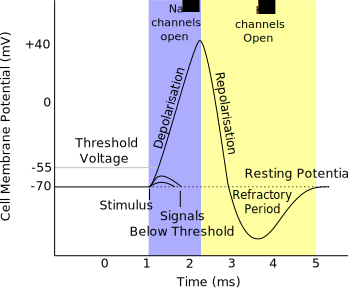
\includegraphics[width=0.5\textwidth]{figures/Hodgkin-Huxley_action_potential.pdf}
	\end{center}
	\captionsetup{singlelinecheck = false, justification=raggedright}
	\caption[The Action Potential is a Solution to the Hodkin-Huxley Model] {\textbf{The Action Potential is a Solution to the Hodgkin-Huxley Model }}{The shape of the action potential is a similar sight in many physiology textbooks. It was is in fact discovered as a result of the mathematical modelling of Hodgkin and Huxley hinting at the deep biophysics of ion channels won them the 1963 Noble Prize in medicine. This discovery is an excellent example of how deep theoretical insight can lead to predictable models of living systems \cite{hodgkin1952, hodgkin1952a, hodgkin1952b, hodgkin1952c, hodgkin1952d}.}
	\label{action_potential_graphic}
\end{figure}

In addition to the mesoscopic models ion channels spawned by hodgkin and huxley, there has been considerable interest in these systems from  the early adopters of computational molecular biophysics. Biophysicists such as Martin Karplus, Beno\^it Roux, Shin Ho-Chung, Mark Sanson, Serdar Kuyucak and Toby Allen have devoted significant parts of their career to studying ion channels\cite{sansom1991, roux1991, sansom1991, allen2003, allen2004, chung2002, tieleman2001}. 

Early studies usually focussed on gramicidin A (gA) as a toy model for the diffusion of charged species. With the advances of this kind of modelling and experimetnal techniques the molecular details of the function of ion channels has become accessible to computational techniques. 

The work on gA enabled careful studies of potassium channels \cite{rashid2013, li2021, vandenberg2021}. Quite rapidly, the availability of protein structures and the maturation of these computational methods has enabled diverse studies of ion channels and other ion channel protein systems \cite{lev2020, chen2021}.


\begin{figure}
	\begin{center}
		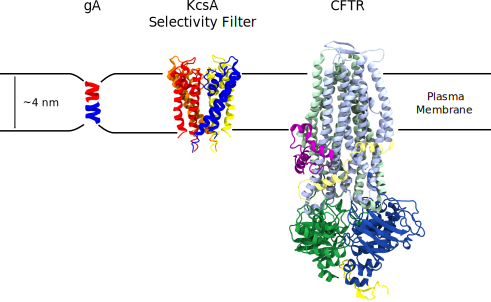
\includegraphics[width=0.8\textwidth]{figures/ion_channel_progression.pdf}
	\end{center}
	\captionsetup{singlelinecheck = false, justification=raggedright}
	\caption[Different Ion Channels Ammenable to Molecular Simulation] {\textbf{Different Ion Channels Ammenable to Molecular Simulation}}{Gramicidin A was initially used as a toy model to test different \textit{in silico} modelling techniques (PDB ID 1NT5) \cite{sham2003}. KcsA, is a bacterial potassium channel. This structure only comprises the pore domain, sometimes called the selectivity filter (PDB ID 1BL8) \cite{doyle1998}. This structure drew interest because potassium channels are critical physiologically. Finally, the CFTR anion channel which this thesis is written about (PDB ID 6MSM) \cite{zhang2018a}. The fact that we have gone from simulating just a few nanoseconds of Gramicidin A to collecting almost half a millisecond of data in this thesis (a time span of 30 years) heralds an exciting future for computational biophysics \cite{roux1993}.}
	\label{action_potential_graphic}
\end{figure}

Until recently, there have been a limited number of structural targets for biophysicists to work with. Initially, inquiries were limited to modelling gramicidin A, an antibacterial peptide which assembles into an ion channel in the cell walls of gram positive bacteria\cite{liou2015}. The mechanism of action for this little peptide is to simply destroy the bacterium's ability to hold an ion gradient. This causes the cell to dis regulate in all sorts of ways, such as the inability to produce ATP.

Gramicidin is one of the toy systems we use as biophysicists to develop theoretical methods. The others being the dialanine peptide, decalanine and sometimes ubiquitin \cite{}.

The discovery of voltage gated channels and a resting potential are still subjects studied in cell biology today as they are critical to the cells' function \cite{}.

These factors have to allowed biophysicists sufficient data to build sufficiently accurate models of protein systems which generalise. Leading to a thriving field, analysing systems as diverse as photocells to gold nano particles CITATIONS NEEDED. \ref{chap:methods}

So by using ion channels as basic biophysical laboratories we can try to understand higher level protein physics \cite{}. In this thesis we will use that higher level understanding to develop a molecular theory of a diseae, Cystic Fibreosis. In future I hope we can use our understanding of protein physics to understand more complex diseases such as diabetes or neurodegenerative diseases. Maybe one day we can build this molecular theory of disease to do medicine with atomic precision.

%=======================================================================================%

\section{Studying Cystic Fibrosis; Toward a Molecular Theory of Disease.} 

The sad truth of Cystic Fibrosis (CF) is that those afflicted are extremely unlucky. A single, change to the genome and their lungs fill with sticky mucus and become infected with bacteria, each breath becomes cumbersome. Personally, I've not met somebody who has this disease. I have consistently wondered what perspective I'm missing by not suffering myself from such a condition or even knowing somebody with it \cite{foucault1994}. Historically diseases have been diagnosed based on symptoms and not causes. As section \ref{} outlines, this is antithetical to how we would like to study physical systems. We would best understand the root cause of a disease so we can predict how to manipulate it. Discovering this root cause can be extremely difficult and often requires decades of clinical enquiry \cite{}. CF has the helpful characteristic of being a monogenic disease, so our molecular theory of this disease only needs to treat a single protein. 

In this way, my motivations for studying the CFTR protein aren't solely focussed on treating disease. This problem is also an interesting opportunity to develop molecular theories of biology. 

There is a perspective on protein evolution which states that the primary sequence of a particular gene contributes to the overall fitness of an organisms by a formula \cite{depristo2005}:

\begin{equation}
	\label{fitness_equation}
	W(\Delta G) \propto \exp\bigg(\bigg[-\frac{\Delta G - \Delta G_{opt}}{\sigma_{\Delta G}}\bigg]^4\bigg) + c
\end{equation}

Here, $W$ represents the evolutionary fitness of an organism, $\Delta G$ is the folding energy of the protein with a given gene sequence and $\Delta G_{opt}$ is the folding energy of the protein in the average (fit) population. The parameter $\sigma_{\Delta G}$ controlls how broad this distribution will be and depends significantly on the protein physics of the gene. Figure \ref{fitness_landscape_gene_figure} demonstrates the types of random walks of a gene through sequence space which this model predicts. 

It just so happens that the CFTR gene exhibits an exceptionally small $\sigma_{\Delta G}$, so the band in the modified gaussian in figure \ref{fitness_landscape_gene_figure} is narrow. This means that CFTR sits at the precipice of a daunting cliff in sequence space. This model is relevant to other diseases as well, such as sickle cell anemia, Alzheimer's disease, and Huntington's disease. So by taking small steps in sequence space and figuring out what factors have caused us to plunge down this cliff, we can try to understand how we might push the needle of protein stability back into the optimal zone.

\begin{figure}
	\begin{center}
		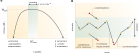
\includegraphics[width=1.0\textwidth]{figures/fitness_landscape_fig.pdf}
	\end{center}
	\captionsetup{singlelinecheck = false, justification=raggedright}
	\caption[A physical model for how to view protein evolution] {\textbf{A physical model for how to view protein evolution}}{a)The stability of a protein $\Delta G$ is related to the fitness of an organism $W$ by equation \ref{fitness_equation}. This model gives rise to a peaked distribution which helps us understand how so many mutants can give rise to cystic fibrosis. It appears as though the CFTR gene has an exceptionally narrow $\sigma_{\Delta G}$ and so small changes to the sequence of the gene have a comparatively dramatic effect on the evolutionary fitness of the organism. b) The model in equation \ref{fitness_equation} Gives rise to a random walk through in sequence space for subsequent generations. In the case of CF it would appear as though \textit{homo sapiens} are stuck at a specific snapshot in evolutionary time where CFTR may easily lose function. So, without gene therapies which can modify a gene sequence \textit {in vivo} we must use a physics based model to somehow broaden the peak in equation \ref{fitness_equation}.}
	\label{dna_structure}
\end{figure}

Moreover, by learning the nuts and bolts of what goes wrong with CFTR we can start to think about where some of these cliffs might be in other places in the proteome, to gain function and avoid disease and debilitation.

The reality of disease pathogenesis being caused by so many different mutations means that there has been decades of investigation into the function of every domain in the protein. 

This theoretical model informs the conclusions of chapter \ref{chap:conclusions}.

Due to the array of disease causing mutations which occur across the cystic fibrosis protein, there is a large body of literature on its unique function \cite{csanady2019a}. This allows us a glance into its function and an opportunity to simultaneously perform basic biophysical research while directly assisting in furthering patient outcomes. This is the sort of inquiry which drives basic science forward, combining interesting experimental data into theoretical models to make testable predictions. The aim of this thesis is to build a model to make predictions about which kind of drugs will produce positive patient outcomes.

As we will see in chapter \ref{chap:cftr} the integration of basic biology into the treatment of cystic fibrosis has drastically improved patient outcomes. The opportunity of this thesis to shed light on the molecular details of this disease could lead to much greater patient outcomes. 

\section{The Future is Biological}
We are on the cusp of developing biology from a descriptive to a predictive science \cite{kochanski1973,liu2005, mogilner2016, covert2021, jumper2021}. This transition is driven by the refinement of experimental techniques, rich datasets, strong theories and powerful computational engines to link the two. As an example of what will soon be possible. Biological systems has happened upon ingenious problems to some very difficult problems through evolution. It has much of the hard work for us and as we understand it better we can begin to apply its logic to our own problems \cite{benyus2009}.

Throughout science, the integration of experimental data with theoretical models leads to new and exciting research, this is particularly true in biology with its important applications in medicine, agriculture and increasingly, manufacturing \cite{anonymous2019, scown2022}. Wet lab biologists take advantage of experimental techniques which allow them to understand the dynamics and structure of living things from the top down. The finer the experimental instrument, the finer the detail they may resolve. Conversely, computational and theoretical biologists take a bottom up approach. We aim to take the granular details of a system, and integrate them upwards to model the macroscopic behaviour of that system. With more powerful computers and more detailed models we can make predictions about the behaviour of more complex systems. What is so exciting about the current era of biological research is that the domains of these two approaches are beginning to overlap, where they can synergize  and drive further breakthroughs. As we discover more systems where this overlap can be found we will develop more sophisticated treatments for diseases and global problems \cite{anonymous2019}.

The reason this has happened before in physics is two fold. The systems physicists usually study are are much more homogeneous. So it's much easier to integrate their formalisms upward. Once we understand the initial conditions and the formalism underlying the interactions in a system it is simply a question of whether or not we have the theoretical and computational capacity to predict the bulk behaviour of that system. 

The difference with biological systems is that they have so many different components that finding an analytic or even computationally tractable solution is usually impossible. However, as we collect more data and build more powerful computers we can approach more complete models. These in turn inform more powerful theoretical models these help direct the material efforts of experimental expertise . 

While previously, we were limited it functional data concerning ion channels we now have unprecedented resolution for the structure dynamics for the inside of a cell. The development of an array of experimental techniques\footnote{Important biophysical techniques which one will encounter often in the literature are cryogenic electron microscopy (Cryo-EM) \cite{cheng2015}, electrophysiology \cite{aidley1996}, nuclear magnetic resonance (NMR) spectroscopy \cite{marion2013}, confocal and fluorescence microscopy \cite{sanderson2014}, X-ray Crystallography \cite{frauenfelder2010}, and genetic engineering (CRISPR-Cas9 or inverse PCR) \cite{silva2017, crispr2019}} has allowed us to allow us to glimpse with unprecedented clarity, the salty dance of life inside our cells.

Alphafold is a good example. This new breakthrough builds on decades of inquiry from the structural biology community and advancements in AI to give high resolution protein structures. Now this result can be used to fill in the gaps of structural biology. Crucually, alphafold konws what it doesn't know. So we can tell where to direct the efforts of structural biology. Together these advances will fill more gaps in our knowledge of protein physics. 

Armed with this philosophy we will delineate how to use the formal object of the Schr\"oedinger wave equation to make approximations to atomic systems in order to create a biophysical model for macromolecular systems like proteins.

\chapter{From Protons to Proteins: Methods to simulate the inside of a cell.}
\numberwithin{equation}{chapter}

\label{chap:methods}

\chapquote{Nature isn't classical, dammit, and if you want to make a simulation of nature, you'd better make it quantum mechanical, and by golly it's a wonderful problem, because it doesn't look so easy.}  {- Richard P. Feynman \cite{feynman1982}}

This chapter is written for somebody who has studied undergraduate physics and now wishes to model biological systems at the molecular level. Care is taken to dive deeper into the mathematical formulations of simulation methods than is conventionally given in introductory texts. Essentially, this is the understanding of simulation techniques I wish I had when I started studying them. An excellent overview which I would recommend as first reading for any new student can be found in an article by Braun et al. \cite{braun2019} followed by Gapsys et al. \cite{gapsys2020} or Grossfield et al. \cite{grossfield2019} for statistical rigour, and Pohorille et al. \cite{pohorille2010} or Chipot \cite{chipot2007} for free energy calculations.  

\section{Quantum Mechanics is Not Tractable at the Scale of Biology.}
Living things are made of atoms, and atoms themselves are composed of many particles, protons, neutrons and electrons. The motions these constituent particles are governed by quantum mechanics. Unfortunately, performing simulations for the number of atoms involved in proteins and other cellular components at quantum mechanical level is impossible. Therefore, we will show how to take the fundamental formulation of atomic interactions in the Schr\"{o}dinger wave equation and apply approximations in order to produce a model which is capable of simulating macromolecular systems at biologically relevant timescales. 

We will gradually integrate upwards, beginning with the interactions in a single molecule we will work our way up to a complex macromolecular system with lipids, water, salts and of course, proteins. Ultimately this section rationalises the treatment of atoms as point charges in classical molecular dynamics simulations. 

\subsection{A full quantum mechanical treatment}
Since we are dealing with atoms which are governed by quantum mechanics we must begin our journey upwards with the time dependent form of the Schr\"{o}dinger wave equation

\begin{equation}
i\hbar \frac {\partial}{\partial t} \Psi (\textbf{x},t) = \big[ -\frac{\hbar ^2}{2m}\nabla^2 + V (\textbf{x}, t) \big] \Psi (\textbf{x},t).
\label {schordinger_time_dependent}
\end{equation}

In quantum systems we treat all particles as waves hence the use of the wave function $\Psi (\textbf{x},t)$. The complex amplitude of the wave function $|\Psi (\textbf {x}, t)|^2$ tells us the likelihood of detecting the particle at time $t$ and at position $\textbf{x}$. The term in the brackets correspond to $-\frac{\hbar ^2}{2m}\nabla^2 $, the kinetic energy of the particle with mass $m$ while $V (\textbf{x}, t)$ is an externally applied potential on the system. Given that the left hand term $i\hbar \frac {\partial}{\partial t} \Psi (\textbf{x},t)$ contains a gradient with respect to time, it governs how the wave function will evolve in time.

When the external potential $V$ has no explicit dependence on time, this equation reduces to the familiar time independent form

\begin{equation}
	E \Psi (\textbf{x}, t) = \big[ -\frac{\hbar ^2}{2m}\nabla^2 + V (\textbf{x}) \big] \Psi (\textbf{x}, t) = H \Psi(\textbf{x}, t).
 \end{equation}

Here, $E$ is an eigenvalue of the Hamiltonian operator $H$. Note that the wave function $\Psi (\textbf {x}, t)$ is still allowed to evolve in time. 

In atomic systems there are two types of particles, nuclei which we will denote with the subscript $n$ and electrons denoted by $e$. In order to treat these elements separately we decompose the Hamiltonian of the system into a few components 

\begin {equation}
H = \underbrace{T_n + U_{n-n}}_{H_n} + \underbrace{T_e +  U_{e-e} + U_{n-e}}_{H_e},
\end {equation}

where $T_n$ and $T_e$ denote the kinetic energy of the nuclei and electrons respectively. While $U_{n-n}, U_{n-e}, U_{e-e}$ denote the potential energy for interactions between nuclei, between electrons and nuclei, and between electrons respectively.

Since the potential terms all describe charged species, they follow Coulomb's law and have the form

\begin{equation}
	U_{n-n} = \sum_{i>j} \frac{q_e^2 z_i z_j }{|\textbf{R}_i-\textbf{R}_j|},\quad U_{n-e} = -\sum_{i,l} \frac{q_e^2 z_i }{|\textbf{r}_l-\textbf{R}_i|},\quad  U_{e-e}  = \sum_{l>k} \frac{q_e^2 }{|\textbf{r}_l-\textbf{r}_k|}.
\end{equation}

Here the $z_i$ represent the atomic number (and thus the charge) of the $i$th nucleus and $q_e$ is the unit charge of the electron. The reason for the separate coordinates $R_i$ and $r_l$ is to separate out the treatment of nuclei and electrons, which will be important once we apply the Born-Oppenheimer approximation.

Meanwhile, the kinetic energy terms are of the form 

\begin {equation}
T_n = - \sum_i \frac{\hbar^2}{2M_i} \nabla_i ^2,\quad  T_e = - \sum_l \frac{\hbar^2}{2m_e} \nabla_l ^2,
\end {equation}

where $M_i$ represents the mass of the $i$th nucleus and $m_e$ represents the mass of an electron. The operator $\nabla^2 = \frac{\partial^2}{\partial x^2} + \frac{\partial^2 }{\partial y^2} + \frac{\partial^2}{\partial z^2} $. The separate subscripts $i$ and $l$ are due to the different coordinates which we use to denote the positions of the nuclei and the electrons. The reason for this will become clear when we derive the Born-Oppenheimer approximation to separate the wave functions and treat them separately.

\subsection{The Born-Oppenheimer approximation.}
\label{born-oppenheimer}
In order to reach the Born-Oppenheimer approximation, we start with the observation that electrons have a mass 3-4 orders of magnitude smaller than the nuclei. This motivates two simplifications. The ``clamped nuclei assumption" where we solve the Schr\"odinger equation whilst nuclei are fixed in space and do not move. And a related assumption known as the ``adiabatic assumption" which postulates that the electrons will respond instantaneously to any changes in the positions of the nuclei. Combining these physical approximations we derive the ``Born-Oppenheimer approximation" for the Schr\"odinger equation which can be used to simplify calculations involving several atoms at once. 

We begin the derivation by examining the time-independent form of the electronic Schr\"odinger wave equation where the nuclei are fixed at positions $R_i$

\begin{equation}
	H_e(\bold{r}_l, \bold{R}_i)  \psi_e (\bold{r}_l,\bold{R}_i)  = U_e(\bold{R}_i) \psi_e (\bold{r}_l,\bold{R}_i).
\end{equation}

Fixing the nuclei in this way gives the ``clamped nuclei" approximation \cite{sherrill}. To solve the wave function for the whole system $\Psi_{tot}$, we use an \textit{ansatz} which decomposes the wave function with an electronic basis into two components: $({\psi_e})_k$ and $({\psi_n})_k$ which are the $k$th eigenfunction solutions to $H_e$ and $H_n$, respectively

\begin{equation}
	\Psi_{tot} (\bold{r}_l,\bold{R}_i, t) = \sum_{k=0}^\infty {\psi_e}(\bold{r}_l, \bold{R}_i)_k\ {\psi_n}(\bold{R}_i)_k.
\end{equation}

Note that there is an implied direct product between the wave functions $\psi_e(\bold{r}_l, \bold{R}_i)$ and $\psi_n(\bold{R}_i)$. When we substitute this expression into the full Schr\"odinger equation \ref{schordinger_time_dependent} we find the following expression for the $k$th nuclear eigenfunction \cite{miller1976} 

\begin{equation}
	i \hbar \frac{\partial} {\partial t} {\psi_n(\bold{R}_i)}_k = \Big[- \sum_i \frac{\hbar^2}{2M_i} \nabla^2_i  + {U_e} (\bold{R}_i)_k\Big] \psi_n (\bold{R}_i)_k + \sum_j C_{kj} \ {\psi_n(\bold{R}_i)}_j,
	\label{adiabatic_approx}
\end{equation}

where we have coupled the electronic wave functions to each other with the operator 

\begin{equation}
	C_{kj} = \int ({\psi_e})_k ^* \Big[\sum_i\frac{\hbar^2}{2M_i}\nabla^2_i\Big] ({\psi_e})_j d\bold{r}  + \frac{1}{M_i}\sum_{i}\bigg[ \int({\psi_e})_k ^* [-\hbar i \nabla_i]({\psi_e})_jd\bold{r}\bigg] [-\hbar i \nabla_i].
\end{equation}

Using the ``adiabatic assumption" \cite{miller1976}, the off-diagonal terms of $C_{kj}$ can be set to $0$ as they represent the interactions between the electrons and the nuclei. This completely decouples the wave function into two components 
\begin{equation}
	\Psi_{tot} (\bold{r}_l,\bold{R}_i, t) = {\psi_e}(\bold{r}_l, \bold{R}_i)_k\ {\psi_n}(\bold{R}_i,t)_k.
\end{equation}

A further approximation is justified by ignoring the diagonal terms $C_{kk}$ as they are 4 orders of magnitude smaller than the other terms in equation \ref{adiabatic_approx} \cite{sherrill}.

We now write the Born-Oppenheimer approximated wave equation for an atomic system  

\begin{equation}
	\label{BO_approx_finished}
	i\hbar \frac{\partial}{\partial t} \psi_n(\bold{R}_i)_k = \big[ -\sum_i \frac{\hbar^2}{2M_i} \nabla^2_i + U_e(\bold{R}_i)_k\big] \psi_n(\bold{R_i})_k.
\end{equation}

The separation between atoms in a molecule is on the order of $10^{-10}m$, while the de Broglie wavelength of the nuclei at room temperature is on the order of $10^{-11}m$. Hence, we treat the nuclei as point particles at the scale of the full molecule. So, by rearranging equation \ref{BO_approx_finished} and taking the derivative with respect to time, we can see how to use Newton's equations of motion to calculate the forces on the nuclei from the surrounding electric potential 

\begin{equation}
	M_i \ddot{\bold{R}}_i (t) = -\nabla_i U_e (\bold{R_i}).
	\label{Newtons_equations}
\end{equation}

By choosing an appropriate time-step, one can simply iteratively solve this equation of motion to understand the dynamics of an atomic system. The nuclei will move according to their relative positions to each other and the electron clouds will rearrange in response to that motion. There is no need to explicitly treat the electrons at all. This is sufficient accuracy to simulate the low energy motions of molecules such as the environment found in biological systems. 
%\begin{equation}
%	(H_n + H_e + V_{n-e})  (\psi_e (\bold{r}_l,\bold{R}_i) \psi_n(\bold{R}_i)) =  (E_n  + U_e)(\psi_e (\bold{r}_l,\bold{R}_i) \psi_n(\bold{R}_i) ) 
%\end{equation}
%

%disregard $T_e$, $V_{n-e}$ and $V_{e-e}$ as they will be close to 0 compared to $T_n$ and $V_{n-n}$.

%In the case of hydrogen we lose an order of magnitude so the approximation is less valid, especially at room temperature. CITATION NEEDED


%
%\begin {equation}
%\Psi(R_i,t) = \psi_e (r_l,R_i) \psi_n(R_i,t)
%\end {equation}
%
%The BO assumption means that we can neglect the cross terms from this separation and treat each wave function independently.
%
%\begin {equation}
%T_n + T_\Psi(R_i,t) = \psi_e (r_l,R_i) \psi_n(R_i,t)
%\end {equation}


\section{Classical MD; Molecular Motions Without Quantum Mechanics}
Following the Born-Oppenheimer approximation there are Hartree-Fock methods and density functional theory (DFT) which further simplify Schro\"edinger's equation. These more sophisticated physical methods allow us to simulate the organisation of electron clouds around small molecules, finding broad applications in chemistry and materials science \cite{vanmourik2014}. These methods are known as \textit{ab initio} MD. 

However, even with these approximations, simulating a large number of atoms is still not computationally tractable. State of the art DFT methods can only simulate on the order of $10^3$ atoms \cite{luo2020} and scales as $O(N^3)$ \cite{kresse1996}. This is not sufficient to simulate proteins and their surrounding solvation environment where the molecular system is usually on the order of $10^4-10^6$ atoms. So, we must use another round of approximations to reach the spatial and time scales necessary to simulate biological molecules. We do this by creating a set of mathematical functions to simplify the calculations further. Here we use a set of virtual springs and other simple models for the energetic interactions between atoms. This creates what's known as an effective potential. 


The CHARMM effective potential employed in all simulations in this thesis is similar to those found in all-atom classical molecular dynamics forcefields. The same functional forms are used in other forcefields such as AMBER, GROMOS and OPLS but with different parameters and design philosophies\cite{lemkul2020}. 

This formulation gives us classical molecular dynamics, sometimes referred to as molecular mechanics (MM). The aim of the classical forcefields discussed here is to use \textit {ab initio} MD as an initial target for approximation and then refine the model to better match certain experimental quantities. This is discussed in detail in section \ref{forcefields_review}.

We split up the molecular mechanics potential into several components dealing with the energies from covalent bonds, including bond stretching, twisting and bending as well as contributions associated with the forces that atoms exert on each other when they are not bonded together 

\begin{equation}
	U_{CHARMM} = \underbrace{U_{LJ} + U_{coulomb}}_{U_{non-bonded}} + \underbrace{U_{bonds} + U_{angles} + U_{dihedrals} + U_{impropers}}_{U_{bonded} }.
	\label{CHARMM_effective_potential_eq}
\end{equation}

Interestingly, the bonded terms may be reasonably approximated by simple harmonic functions, with an exception we will discuuss shortly, 

\begin{equation}\label{bonded_eqs}
	\begin{aligned}
	U_{bonded} = \sum_{bonds} k_{b} (b-b_0)^2 + \sum_{angles} k_\theta(\theta-\theta_0)^2+ \sum_{Urey-Bradley} k_u(r_{UB}-r_{UB_0})^2   \\ + \sum_{dihedrals} k_\varphi (1+\cos(n \varphi - \delta)) + \sum_{improper-dihedrals}  k_{\phi} (\phi - \phi_0)^2.
\end{aligned}
\end{equation}

Here, the $k_i$ terms correspond to the strength of the restraint for a parameter. The $0$ subscript denotes the equilibrium position for that parameter. Even though this formulation is quite simple, it has empirically been shown to be a reasonable approximation for the potential energy functions of quantum mechanics in covalently bonded chemical species. Examples can be seen in figure \ref{QM_MM_compared}.

Over time several additions have been made to this formalism in order to reproduce experimental measurements of chemical systems \cite{mackerelljr.2004}. We will discuss two of the major additions to the CHARMM formalism. The first is energy correction maps, abbreviated ``CMAP corrections" concerning the dihedral parameters\cite{mackerell2004, mackerell2004a}. These were motivated by the observation that MD simulations were not correctly reproducing protein secondary structure and resulted in errant Ramachandran distributions \cite{ramachandran1963, mackerell2004}. Mathematically, these corrections take the form of a two dimensional grid which is used to interpolate results from \textit{ab initio} quantum mechanics calculations for the torsion angles. Continued adjustments to $U_{dihedral}$ in the form of these CMAP corrections have resulted in substantial improvements to the CHARMM forcefield, particularly for disordered proteins \cite{huang2016}. 

There have also been additions of ``non-bonded fix" or ``NBFIX"  corrections to the Lennard-Jones parameters in CHARMM. NBFIX parameters modify the Lennard-Jones parameters between \textit{specific} atom types. For example, in order to reproduce experimental values of osmotic pressure for sodium chloride, the values of $\epsilon$ and $\sigma$ are modified  values \textit{only} when calculating the Lennard-Jones potential between sodium and chloride atoms. These modifications fixed issues with certain charged species, such as sodium and chloride, which were associating too much in bulk solution or the overly stable salt bridges within proteins \cite{yoo2018, tolmachev2020, huang2016, savelyev2015}.

\begin{figure}
	\begin{center}
	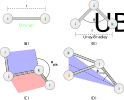
\includegraphics[width=10cm]{figures/bonded_interactions.pdf}
	\end{center}
	\captionsetup{singlelinecheck = false, justification=raggedright}
	\caption[The Bonded Interactions Calculated In Classical Forcefields]{\textbf{The Bonded Interactions Calculated In Classical Forcefields.}}{
	(A) The energy of Bond Stretching is approximated as a harmonic oscillator with respect to their separation $r$. (B) Angles between neighbouring covalently bonded atoms are also approximated as a harmonic oscillator with respect to the angle $\theta$. In some forcefields such as CHARMM there is a correction term for these angular interactions known as Urey Bradley forces. This is calculated using the separation between the non-bonded atoms $i$-$k$ in the triplet with the parameter $r_{UB}$. (C) The dihedral angle between four atoms is calculated by constructing two planes. Each plane is constructed to contain three of the four atoms in the set. One plane encompasses atoms $i, j$ and $k$ here colored in blue and the other plane contains the $j$, $k$ and $l$ atoms colored in red. The dihedral angle is then calculated by taking the angle between these two planes along the line they intersect, the line formed by the $j$-$k$ bond. (D) The improper dihedral angles enforce the planarity of a molecular configuration. A plane is constructed to contain the $i$, $j$ and $k$ (blue) atoms and another plane is constructed to contain the $j$, $k$ and $l$ atoms (red). The improper angle is then calculated as the angle between these two planes. }
	\label{charmm_bonded}
\end{figure}

\subsubsection{Non Bonded Interactions}

The term $U_{non-bonded}$ captures interactions which arise when atoms are not covalently bound to each other. Namely, Coulomb forces due to electric charges on the atoms, attractive Van Der Walls interactions and repulsion due to Pauli Exclusion,
\begin{equation}\label{nonbonded_eqs}
	\begin{aligned}
		U_{non-bonded} = \underbrace{\sum_{i>j} \epsilon_{ij} \Big( \Big(\frac{\sigma_{ij}}{r_{ij}}\Big)^{12} - \Big(\frac{\sigma_{ij}}{r_{ij}}\Big)^{6} \Big)}_{U_{Lennard-Jones}} - \underbrace{\sum_{i>j} \frac{q_i q_j } {r_{ij}}}_{U_{coulomb}}. 
	\end{aligned}
\end{equation}

Note how the repulsive Pauli Exclusion and attractive dispersion forces have been combined into one term known as the Lennard-Jones potential or $U_{LJ}$. The $\sigma$ parameter denotes the location of the local minima in the Lennard-Jones potential. This is the optimum distance that two atoms will rest against each other in the absence of other effects. The $\epsilon$ parameter denotes the depth of the potential well, or how stable the two atoms will be in the minimum energy configuration. This is very important for certain physical parameters such as osmotic pressure \cite{yoo2018}.

Meanwhile, the partial charge assignments $q_i$ for each atom are very important in a biological context, for stability of protein conformations of salt bridges and the solvation energy of different molecules \cite{jambeck2013}.

By focussing on adjusting the charges of an atom to fit the solvation energy of a molecule and adjusting the Lennard-Jones parameters to fit the osmotic pressure measurements, we  can isolate and determine these non-bonded parameters fairly well.

\begin{figure}
	\begin{center}
	\includegraphics[width=\textwidth]{figures/QM_MM_compared.pdf}
	\end{center}
	\captionsetup{singlelinecheck = false, justification=raggedright}
	\caption[Comparison Between Potentials in Quantum and Classical Forcefields] {\textbf{Comparison Between Potentials in Quantum and Classical Forcefields}}{ A) The Morse potential was formulated to approximate the potential energy surface associated with the stretching of covalent bonds (blue). At low temperatures (the ground state, $v=0$) like those found in classical MD there is good agreement between the Morse potential and the harmonic oscillator (green) (Credit, Mark Somoza 2006). B) Here the potential of the dihedral angle between the atoms C1,C2,C3 and C4 in a butane molecule is calculated using two methods: Quantum Chemical calculations and approximations using the functional form in equation \ref{bonded_eqs} \cite{lemkul2020}. Note how the appropriate choices of $k_\varphi$, $n$ and $\delta$ have closely approximated the results in the more accurate quantum mechanical calculations.}
 
	\label{QM_MM_compared}
\end{figure}

\begin{figure}
	\begin{center}
		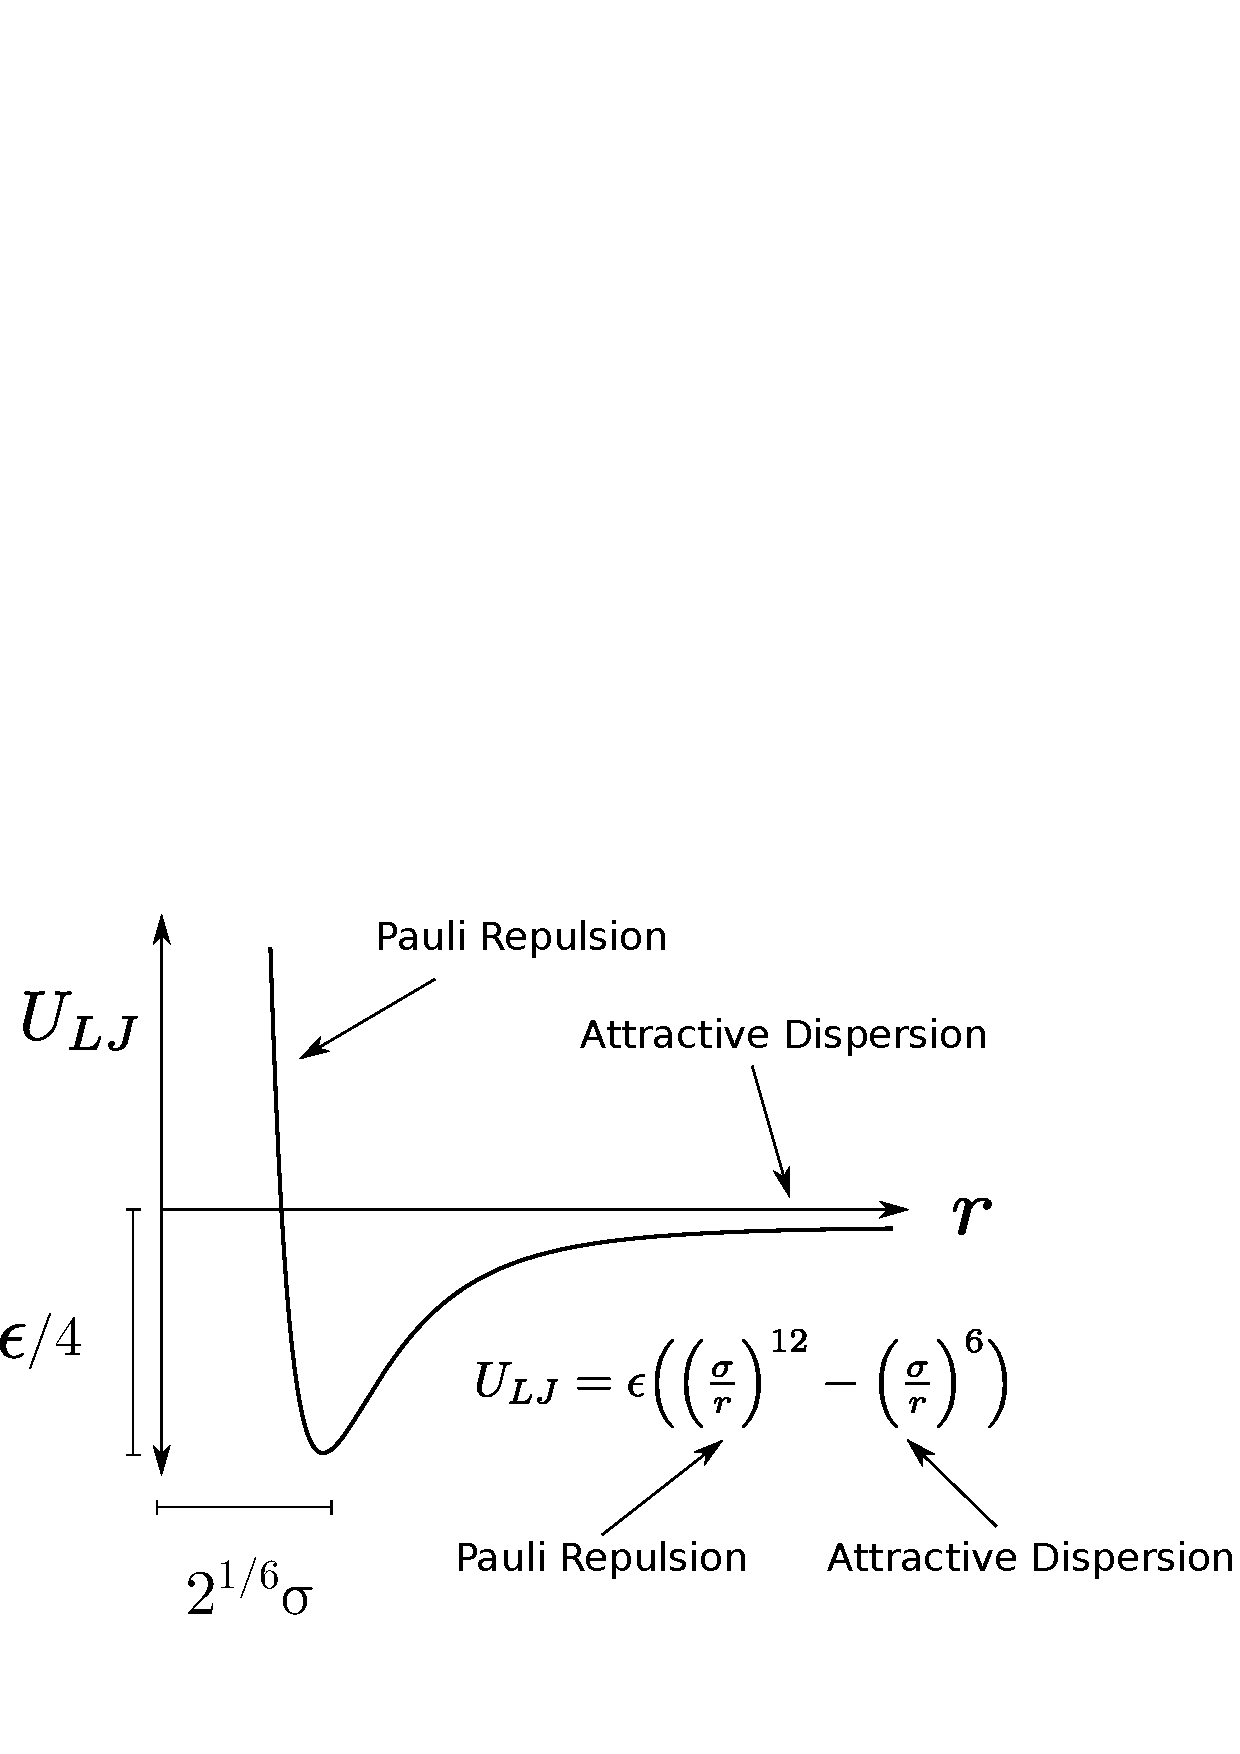
\includegraphics[width=\textwidth]{figures/LJ_figure.pdf}
	\end{center}
	\captionsetup{singlelinecheck = false, justification=raggedright}
	\caption[The Lennard-Jones Potential] {\textbf{The Lennard-Jones Potential}}{A) The Lennard-Jones potential function has two regimes, the far region one dominated by attractive dispersion forces and the close region dominated by repulsion. In the case of atomic systems this is due to the Pauli exclusion principal. B) An example of a fluid modelled with Lennard-Jones particles \cite{chari2019}. C) The radial distribution function ($g$) for a Lennard-Jones fluid \cite{morsali2005}. Note that the peaks in the distribution are spaced roughly 1 $\sigma$ apart. }
	\label{Lennard-Jones_figure}
\end{figure}

\subsection{Philosophy of Different Molecular Mechanics forcefields.}
\label{forcefields_review}
At the time of writing, the four popular forcefields for the simulation of biomolecules are CHARMM, AMBER, GROMOS and OPLS. Each of these have a slightly different philosophy in their formulation. They may be bottom up, as in the case of AMBER and CHARMM or top down, in the case of OPLS. Bottom up forcefields take the results from \textit{ab initio} MD calculations as an initial guess and approximate them by tweaking the parameters in the functional form in equation \ref{CHARMM_effective_potential_eq}. Conversely, top down forcefields tweak these parameters with reference to experimental measurements. Ultimately, the results from \textit{in silico} experiments must match those of wet lab experiments, so the development of all forcefields has elements of both philosophies. All forcefields assign the partial charges to atoms using the results of \textit{ab initio} MD calculations. The rest of the parameters are derived with other methods such as attempting to match the known secondary structures of peptides \cite{huang2016}. Different forcefields have different methods of deriving their parameters. Below is a short summary of the philosophy for the four major forcefields taken from the review by Justin Lemkul \cite{lemkul2020}. 

\begin{itemize}
	\item CHARMM: The most popular all atom forcefield. To build CHARMM, QM optimized geometries and molecular dipole moments are compared to those found from calssical MD simulations. Molecular degrees of freedom such as dihedral angles are also fit with QM energy profiles, an example can be seen in \ref{QM_MM_compared}. Macroscopic experimental quantities are also used to validate the parameters in this forcefield, such as solvation energies, crystal geometries, heats of vaporization and conformational sampling of biomolecules \cite{huang2016}. One of the reasons for this forcefield's popularity is its considerable library of supported compounds, especially when combined with its generalisation module CGENFF \cite{vanommeslaeghe2010}. 

	\item AMBER: An all atom forcefield which is built from the ground up from results from quantum mechanical calculations and results from spectroscopy. A version of this forcefield has become the favorite for the simulation of disordered proteins \cite{robustelli2022, robustelli2018}. There is also a generalised version of the AMBER forcefield known as GAFF \cite{wang2004, wang2006}. Comparisons between generalised forcefields can be found in \cite{zhu2019}.

	\item OPLS: An all atom forcefield. The OPLS forcefield takes the philosophy that, since many biomolecules share similar geometries to certain organic liquids, biomolecules can be accurately parameterised by creating a forcefield which correctly reproduces the experimental measurements for these species. Parameters are derived to accurately reproduce the liquid density of certain organic liquids. These parameters are then used as roots to construct larger biomolecules by drawing analogies between similar molecular geometries. 

	\item GROMOS: A united atom forcefield, where hydrogen atoms are typically merged into the heavy atom they are bound to. Hence, they are not explicitly treated. Charge assignment is done with DFT. Interestingly, GROMOS uses a quartic form of the bond stretching term 
		\begin{equation}
			U_b = \frac{1}{4} k_b (b^2-b^2_0)^2.
		\end{equation}

		The parameters are adjusted for agreement with experimental values such as  solvation energies, liquid densities. GROMOS forcefields are popular in some contexts because of its ability to reproduce partition coefficients between polar and non-polar media, a similar chemical context to what is found at the interface between a membrane and bulk water.

\end{itemize}

\section{Periodic Boundaries To Pretend A Protein is Inside a Cell}
\begin{figure}
	\begin{center}
		\includegraphics[width=\textwidth]{figures/MD_unit_cell_example/MD_system.png}
	\end{center}
	\captionsetup{singlelinecheck = false, justification=raggedright}
	\caption[An Example of a Solvated Biomolecular Environment Ready for Simulation] {\textbf{An Example of a Solvated Biomolecular Environment Ready for Simulation}}{This rendering shows a CFTR protein embedded in a lipid bilayer, immersed in a potassium chloride solvent. Half of the bilayer has been stripped away, as has much of the solvent so the protein is visible. The phospholipid lipid bilayer is colored grey, while the potassium chloride ions are colored pink and yellow, respectively. Water molecules are red and white. The blue box indicates the boundaries of the unit cell. This system contains roughly 190,000 atoms in total.}
	\label{MD_environment}
\end{figure}

Inside cells, proteins are immersed in a large solvation environment composed of water and salts \cite{phillips2012}. An example can be seen in figure \ref{MD_environment}. However, simulating such a large environment is computationally expensive and truncating it with vacuum at the boundaries leads to water molecules aligning their dipole moments along the boundary and perturbing equilibrium dynamics. In order to avoid such artefacts, we have to replicate the large cellular environment somehow \cite{ross2018}. We could make a simulation box large enough to replicate the behavior of a bulk solvent, but even with a large simulation box we can still observe artifacts associated with the vacuum at the boundaries \cite{gapsys2020}. So, to avoid these boundary effects, we use periodic boundary conditions (PBCs), allowing atoms to move between images in the simulation box. This replicates the molecular system infinitely in every direction. 

Using PBCs might remove vacuum from our molecular system but now we have a different problem. Effectively, with the PBCs, we have created a system with an infinite number of atoms. We have to somehow limit the number of computations we perform. We could simply truncate the calculation of interactions $U_{non-bonded}$ after a certain cutoff distance. This is not an issue for $U_{LJ}$ because the $1/r^6$ and $1/r^{12}$ terms in equation \ref{Lennard-Jones_figure} decay very quickly for large $r$. Inaccuracies due to this approximation can be further ameliorated with the use of a smooth switching function \cite{klauda2007, venable2009}. On the other hand, the $1/r$ dependence in $U_{coulomb}$ scales much more slowly so truncating it leads to a loss of accuracy in the results of the simulation \cite{auffinger1995, perera1995, roberts1994, delbuono1996, essmann1995}. So, we have to calculate the contributions of $U_{coulomb}$ in between all periodic images. Note that this periodicity requires that the unit cell is electrically neutral, else the contribution of potential energy from $U_{coulomb}$ will be infinite, leading to artefacts \cite{hub2014}.

\begin{figure}
	\begin{center}
		\includegraphics[width=\textwidth]{figures/PME_miro.pdf}
	\end{center}
	\captionsetup{singlelinecheck = false, justification=raggedright}
	\caption[Particle Mesh Ewald Summation] {\textbf{Particle-Mesh Ewald Summation}}{A)The molecular system is repeated infinitely along all axes, when atoms reach the edge of the simulation box, they are allowed wrap around to the other side of the box. B) The charges in the infinite periodic system are approximated onto a regular grid. Then the potential in the infinite system is calculated via a Fast Fourier Transform (FFT). C) A more detailed view of the charge mapping procedure. The charges in the system are interpolated onto the grid using B-spline interpolation. }
	\label{PME_illustration}
\end{figure}

To calculate $U_{coulomb}$ in all periodic images and limit computational intensity of our calculations we use a clever scheme known as Particle-Mesh Ewald summation (PME). Interestingly, this scheme ends up scaling better than the pairwise summation in equation \ref{nonbonded_eqs} might imply. The direct summation scales with computational complexity of $O(N^2)$  with the number of atoms while the infinite PME scheme scales as $O (N\log N)$ \cite{darden1993}, though there are some further considerations for large systems on parallel architectures \cite{hardy2015}. Even with these sophisticated algorithms, the calculation of electrostatic potential in the infinite system still represents the largest computational bottle-neck in classical MD \cite{hardy2015}.

For a detailed review of different Particle-Mesh Ewald summation methods and the mathematics behind the method see \cite{shan2005}. A brief outline of the Smooth Particle Mesh Ewald summation is given below 

\begin{enumerate}
	\item An \textit{ansatz}  is used where $U_{coulomb}$  has Gaussian screening charges added to it and simultaneously subtracted away to create a smooth potential. The details can be found in \cite{shan2005}.
		\begin{equation}
			\begin{aligned}
			U_{coulomb} &= U_{screening-charges} + U_{coulomb}  - U_{screening-charges}.
			\end{aligned}
		\end{equation}
		Terms in these equations are then rearranged such that one term is evaluated with a Fourier transform and the other term is evaluated using a direct sum.
		\begin{equation}
			\begin{aligned}
			U_{coulomb} &= U_{FT}  + U_{direct-sum}.
			\end{aligned}
		\end{equation}
	\item The charges to be evaluated using $U_{FT}$ are interpolated onto a grid using B-spline interpolation functions. This is the procedure demonstrated in figure \ref{PME_illustration}.
	\item The charge density functions for the charges on the grid are transformed into frequency space using Fast Fourier Transforms.
	\item The Poisson equation is solved numerically in frequency space for these charges.
		\begin{equation}	
			\nabla^2\tilde{U} = 4\pi \tilde{\rho}(\bold{k})
		\end{equation}	
		Where $\tilde{U}$ is the component of $U_{FT}$ we solve for in frequency space and $\tilde{\rho}$ is the Fourier transform of the smooth scalar function for the interpolated charge densities. 
	\item An inverse Fourier transform is calculated for the solution to $\tilde{U}$ to transform it back into real space. 
	\item The interactions in $U_{direct-sum}$ are evaluated using a simple pairwise summation.
	\item Now that $U_{coulomb}$ is known at every position in the unit cell, we can move atoms according to the contributions from this potential using Newton's second law.
\end{enumerate}

\section{Controlling the Temperature and Pressure in a Simulation}
Living things are very sensitive to their external environment. Enzymes only work in a narrow range of temperatures and cells burst apart in the absence of pressure\cite{peterson2007, song2012}. As such, to correctly understand biological systems we not only need to simulate the dynamics of the atoms inside them, but we must also make sure that the virtual environment in our simulations matches what is found inside cells or in the laboratory. Our simulations should seek to approximate the environment of an open topped test-tube sitting in a pressure and temperature controlled laboratory. To do this, we make use of some statistical ensembles chosen for their performance in regulating the thermodynamic quantities in a simulation and their computational expense.  

%Langevin dynamics
%\begin{equation}
%	m_i  \dot{v} _i = F_i + m_i \gamma_i \bold{v}_i + R(t)
%\end{equation}

\subsection{Hot and Cold with the Nos\'e-Hoover Thermostat}
Recall that the temperature of a system is a direct function of the velocity of its constituent particles. So by regulating the ensemble of velocities we can control the temperature. We begin a simulation by choosing the velocities of the atoms within the system from a Maxwell-Boltzmann distribution 

\begin{equation}
	f(v_i) = \Big(\frac{m_i}{2\pi k_B T}\Big)^{3/2} \exp{\Big(-\frac{m_iv_i^2}{2k_BT}\Big)},
\end{equation}

where $f(v_i)$ is the proportion of particles with velocity $v_i$, $k_B$ is Boltzmann's constant. Note that $i=1,...,N_{df}=3N$ as we choose a velocity component for $x,y \ \text{and}\  z$ separately. 

Despite starting from the same Cartesian coordinates, randomly sampling velocities from the Maxwell-Boltzmann means that replicate simulations will immediately begin from different points in phase space. Their coordinates will quickly diverge, raising questions around how long one should run a simulation and how many replicates they should run in order to collect reliable statistics. According to Knapp et al. \cite{knapp2018}, a good rule of thumb is to simulate between 5 and 10 replicates depending on the availability of computing resources\footnote{Recall that in the ergodic limit, a quantity $f$ calculated from the ensemble average of replicates will be equal to the time average calculated from one replicate in the limit $t\to\infty.$ That is $$ \langle f \rangle_i = \lim_{t \to \infty } \frac{1}{t} \int_0^tf(\tau)d\tau $$}. In this thesis we prioritised long time scales to sample slow motions, so 3 replicates with run times between 1 and 2 microseconds were produced for all systems. 

After the initial choice of velocities, the temperature in a simulation is maintained by directly modulating the velocities of the atoms to maintain the target temperature $T_0$. There are many schemes which attempt this. We will discuss the Nos\'e-Hoover thermostat in detail here because it was used during the production runs in this thesis  \cite{nose1984, hoover1985, martyna1992}. However, for the equilibration phase of the simulations, we used the Berendsen thermostat because it is faster at correcting large temperature differentials but does not produce the correct statistical ensemble \cite{bussi2007, berendsen1984}. We also note that the field has since moved on to favor the Bussi thermostat, which is an extension of the Berendsen thermostat, as it works well in most contexts  \cite{bussi2007, braun2019}.

The Nos\'e-Hoover thermostat is characterised by the use of an extra, massive particle coupled to an external bath. The use of a single bath has been associated with issues with ergodicity and so usually this particle is coupled to a chain of external baths. Usually, the software simulation package GROMACS uses a chain of 10 baths, $M=10$ \cite{martyna1992, martyna1996, abraham2015}. The Hamiltonian for the Molecular Dynamics system coupled to a chain of $M$ external baths is then

\begin{equation}
	H_{NH} (\bold{x},\bold{p},\eta_1 , ... , \eta_M, p_{\eta_1}, ...,  p_{\eta_M}  )= H_{MM} + \sum_j^M \frac{p^2_{\eta_j}}{2Q_j} +k_BT  N_{df}   \eta_1   + k_BT \sum_{j=2}^M\eta_j.
\end{equation}

Here, usually $N_{df} := 3N$ unless there are constraints placed within the system to freeze atoms. $\eta$ denotes the 1 dimensional coordinate of the thermostat particle with mass $Q$, while $H_{MM}$ is the Hamiltonian of the unregulated molecular mechanics system 

\begin{equation}
H_{MM}(\bold{x},\bold{p}) = \underbrace{\sum_i^N \frac{\bold{p}_i^2}{2 m_i}}_{E_{kinetic}} + U_{CHARMM} (\bold{x}). 
\end{equation}

By using Hamilton's equations of motion, $H_{NH}$ evolves by

\begin{equation}
	\begin{aligned}
		\dot{\bold{x}_i} &= \bold{p}_i/m_i \\
		\dot{\bold{p}_i} &= \bold{F}_i-\bold{p}_i\frac{p_{\eta_1}}{Q_1} \\
		\dot{\eta_j} &= p_{\eta_j}/Q_j \\
		\dot{p_{\eta_1}} &= \bigg[\sum_i^N \frac{\bold{p}_i^2}{m_i} - N_{df} k_B T\bigg]  - p_{\eta_1}\frac{p_{\eta_2}}{Q_2} \\ 
		\vdots \\ 
		\dot{p_{\eta_j}} &= \bigg[ \frac{p^2_{\eta_{j-1}}}{Q_{j-1}} - k_bT \bigg]  - p_{\eta_{j}}\frac{p_{\eta_{j+1}}}{Q_{j+1}} \\ 
		\vdots \\ 
		\dot{p_{\eta_M}} &= \bigg[ \frac{p^2_{\eta_{M-1}}}{Q_{M-1}} - k_bT \bigg],
	\end{aligned}
	\label{NH_equations}
\end{equation}
where $\bold{F}_i$ is the force vector on the $i$th particle. It may be calculated from $U_{CHARMM}$ using Newton's second law. 

The parameters $Q_j$ are chosen by the user to control the coupling strength of the baths to each other. We usually choose   
\begin{equation}
	Q_j = \frac{\tau_{NH}T_0}{4\pi^2}\qquad  \forall j,
\end{equation}
where $\tau_{NH}$ is the time interval between when the thermostat parameters are updated. This means that whenever the simulation is not at a time step that is a multiple of $\tau_{NH}$,  we can just evaluate $U_{CHARMM}$ as normal but every interval of $\tau_{NH}$, we rescale the velocities according to the equations of motion in \ref{NH_equations} to match the correct temperature $T$.

Remember that we can always calculate the temperature using the instantaneous velocities in the simulation using

\begin{equation}
	\begin{aligned}
		T &= \frac{2E_{kinetic}}{3Nk_B}  =  \frac{\sum_i m_i v_i^2}{3Nk_B} 
	\end{aligned}
\end{equation}
	
The Nos\'e-Hoover thermostat, when chained infinitely, allows us to  accurately produce what's known as an NVT ensemble, also called the canonical ensemble in the statistical mechanics literature \cite{martyna1992}. Where the number of particles in the system (N) remains constant, the volume of the system remains constant (V) and the temperature remains constant (T). In a realistic environment, the pressure remains constant rather than volume, so we need another regulatory mechanism to modulate the volume of the system to regulate the pressure (P) and produce an NPT ensemble. 

\subsection{Under Pressure with the Parinello-Rahman Barostat}
Pressure is critical to the function of living organisms. Membranes burst apart at low pressures \cite{karal2021} and at high pressures cellular function is disrupted \cite{macdonald2001}. In order to accurately reflect the atmospheric pressure at which living things thrive we have to accurately calculate and modulate it during our simulation.

In order to measure the pressure at the simulation walls, we follow the procedure in \cite{allen1991} by calculating a quantity known as the virial:

\begin{equation}
	W(\bold{x}) = \sum_i^{N-1} \sum^N_{j>i} \bold{r}_{ij} \cdot \bold{F}_{ij},
\end{equation}

where $\bold{r}_{ij} = \bold{x}_i - \bold{x}_j$  is the Cartesian distance between the $i$th and $j$th atoms, while $\bold F_{ij}$ is the force extorted on atom $j$ by atom $i$. 
This is then substituted into the equation 

\begin{equation}
	P (\bold{x}) = \frac{N k_B T + \langle W \rangle_i}{V}
	\label{instantaneous_pressure}.
\end{equation}

And so using equation \ref{instantaneous_pressure}, we can modulate the volume $V$ of the simulation in order to control the pressure throughout the simulation.

For this purpose, we apply the Parrinello-Rahman barostat \cite{parrinello1980, parrinello1981}, using a procedure with a similar philosophy to the extended Hamiltonian used in the Nos\'e-Hoover thermostat. In this case, the system is coupled to an external pressure bath rather than an external temperature bath. First we define that the basis vectors for the periodic simulation box as $\underline{h}:= [\bold{a}, \bold{b} ,\bold{c}]$. When the box is scaled to change the volume these basis vectors are multiplied by a set of scalars $s_i := (\xi_i$, $\eta_i, \zeta_i ) \in [0,1]$. We perform a change of coordinates so that the contributions of the particles onto the boundaries is easily calculated from our equations so we express the atomic coordinates as

\begin{equation}
\begin{aligned}
	\bold{x}_i &= \xi_i \bold{a} +\eta_i \bold{b} +\zeta_i \bold{c}  \\
	           &= \underline{h}\bold{s}_i.
\end{aligned}
\end{equation}

Defining $\underline{G} := \underline{h}^T\underline{h}$, the Lagrangian for the scaling system then becomes
\begin{equation}
\begin{aligned}
	L = \frac{1}{2} \sum_i^N \  m_i \dot{\bold{s}}_i^T\underline{G}\dot{\bold{s}}_i - \sum_i \sum_{j > i } \phi (\bold{r_{ij}}) + \frac{1}{2} \ M \text{Tr}(\dot{\underline{h}}^T\dot{\underline{h}})   - {P}_{ext} V,
\end{aligned}
\end{equation}

where $\phi(\bold{r}_{ij}$ is the pairwise potential between two atoms in $U_{CHARMM}$, while $M$ is a constant of proportionality associated with the kinetic energy derived from the movement the particles undergo as they scale. It has units of mass. $P_{ext}$ is our target, externally applied pressure. This Lagrangian allows us to derive the equations of motion  

\begin{equation}
\begin{aligned}
	\ddot{\bold{s}}_i &= -\sum_{j\neq i}   \frac{1}{m_i\bold{r}_{ij} }\frac{d\phi(\bold{r}_{ij})}{d r_{ij}}  (\bold{s}_i - \bold{s}_j) - G^{-1}\dot{G} \dot{\bold{s}}_i \\
	\ddot{\bold{h}} &= \frac{1}{M} (\bold{Y} -P_{ext}) \underline{\sigma}.
\end{aligned}
\end{equation}
The matrix $\underline{\sigma} := V (\bold{h}^T)^{-1} = V  [\bold{b} \times \bold{c}, \bold{c} \times \bold{a}, \bold{a} \times \bold{b}] $  contains information about the size and orientation of the simulation box, while 

\begin{equation}
\begin{aligned}
	\bold{Y} = \frac{1}{V}\sum_i m_i (\underline{h}\dot{\bold{s}}_i) (\underline{h}\dot{\bold{s}}_i)^T + \sum_i \sum_{j>i}\frac{1}{{r}_{ij}} \frac{d \phi (\bold{r}_{ij})}{dr_{ij}} \bold{r}_{ij}\bold{r}_{ij}^T,
\end{aligned}
\end{equation}

represents the stress tensor which acts across each of the faces of the unit cell. 
This system of equations can be solved numerically to control the pressure of the simulation system by modulating the length of the basis vectors $\bold{a}, \bold{b}$ and $\bold{c}$ contained in $\underline{h}$.

	Together with the Nos\'e-Hoover thermostat, the Parrinello-Rahman barostat produces NPT, also called the isothermal-isobaric ensemble in the statistical mechanics literature. The combination of these two methods is thus appropriate for simulating a cellular environment. 


	\section{The Process of Preparing an MD Simulation}
	The process of taking a molecular structure and putting it in a cellular environment to simulate it at physiological temperatures is both an art and a science. It's a science because a biophysicist must be aware of the many tricks that structural biologists use to image a macromolecular complex. But it's an art because accounting for those tricks and making the necessary modifications is rarely straightforward. How do you build a missing loop? What charge state is an amino acid most likely to take in a physiological context? These questions must be carefully answered by analysing the literature about the system of interest. Once the protein structure has been built, the system is immersed in a water solvation bath alongside a concentration of salt ions, usually sodium chloride if the environment is thought at be extra cellular or potassium chloride if the environment is thought to be intracellular. Once the initial conditions have been decided, we need to make a few preparatory steps so the simulation collects reasonable results and doesn't hurtle along some unphysical trajectory. The steps so that the simulation remains realistic are fleshed out in some more detail in \cite{braun2019} but we produce a short summary below.

	\begin{enumerate}
		\item Minimisation: Here the atoms are moved down along $U_{CHARMM}$ to resolve any clashes in the system which would cause LINCS or SHAKE to diverge. This is usually done with simple minimisation algorithms such as steepest descent or conjugate gradient descent \cite{leach2001}. This performed while the simulation box has a fixed volume. 
	\item Relaxation: Harmonic restraints are placed on the heavy atoms (non hydrogen) in the system so that large conformational changes do not occur while the macromolecules are heated and settle into their solvation environment. This may be done under the NVT or NPT ensembles depending on the system. Sometimes the system is heated slowly from 0 Kelvin up to the desired thermal temperature in order to avoid large conformational changes which might result from different parts of the system heating at different rates. 
\item Equilibration: Often after relaxation more simulation time is run so that the system can settle into local minima further. This process makes sure that the physically relevant local minima are being sampled once we move to production. This process could be run for a few nanoseconds or up to a microsecond. It depends on the system. This is usually done with the NPT ensemble.
\item Production: Here the NPT ensemble is applied and the system is allowed to evolve under Newton's equations of motion while data is collected for analysis.
\end{enumerate}


\section{Choosing an Appropriate Time Step}
The discrete time step, $\Delta t$ which is used to integrate our equations of motion is one of the most important determinants in the performance of the simulation. We would like $\Delta t$ to be as large as possible, so that the minimum number of calculations are made to sample the desired time scale. In the case of proteins this usually runs between $10^{-6}$ and $10^{-3}$ s \cite{robustelli2022}.  

As you can see in table \ref{timescales} the fastest motion in molecular systems is dictated by stretching of covalent bonds. Studies of the resonance of molecules by infrared spectroscopy determined that the O-H type bonds oscillate the fastest, with a resonance peak at 3600 cm$^{-1}$\cite{schlick2010}. 

Due to Nyquist's theorem the largest $\Delta t$ parameter we can choose \textit{must} be less than half the speed of the fastest degree of freedom in the system \cite{shannon1949}. However, empirically we have found that condensed matter systems require even shorter time steps to maintain their stability \cite{leach2001}. The Verlet leap-frog scheme used in most MD codes requires between 5 and 10 integration steps per period of the fastest harmonic mode in a system, to maintain stability \cite{mazur1997, feenstra1999}. The choice of too large a time step means that the system will escape local free energy minima, accumulating kinetic energy and eventually ``blow-up" \cite{braun2019}. In the case of biomolecular systems we are challenged by the fact that they are so hydrogen-rich. Since hydrogen is so light, its motion is much faster compared to the other molecular motions involving heavier, slower moving atoms. Its correlation time is on the order of 1 femtosecond. In classical simulations we are able to get away with using 2 femtoseconds with the use of specialised integration schemes such as SHAKE\cite{andersen1983} and LINCS\cite{hess1997} to constrain the fast motion of hydrogen atoms. This allows us to use $\Delta t = 2$ fs in atomistic classical MD simulations.

The use of techniques such as hydrogen mass repartitioning \cite{balusek2019}, virtual site topologies \cite{feenstra1999} and multiple time step schemes \cite{streett1978} have also gained popularity in recent years in order to increase time steps further, up to $\Delta t = 5 $fs. 

\begin{table}
	\begin{center}   
		\begin{tabular}{ |c|c|c|}
			\hline
			Motion & Timescale \\
			\hline
			Covalent Bond-stretching & $1-2\times10^{-15}$ s \\
			Covalent Bond-angle bending & $5-10\times10^{-15}$ s \\ 
			Sidechain  Motions & $10 ^{-12}-10^{-6}$ s \\
			Rigid Body Motions & $10 ^{-9}-1$ s \\
			Ion Conduction & $10^{-9}-10^{-6}$ s \\
			Protein Conformational Changes & $10^{-9}-10^{-3}$ s \\
			Alpha Helix Formation & $10^{-9}-10^{-6}$ s \\
			Beta Sheet Formation & $10^{-6}-10^{-3}$ s \\
			Protein Folding & $10^{-6}-10$ s \\
			\hline
		\end{tabular}
\end{center}
%\begin{tabular} { |c|c|c| } 
%	\hline
%	%\label{atomic_motions_speed}
%	System Description & Fastest Degree of Freedom & Characteristic Timescale \\ 
%	\hline
%	Uncoupled Atoms  & Atom Translation & 10 fs  \\ 
%	Rigid Molecules & Rigid Body Rotation & 5 fs \\  
%	Flex. Molecule with Rigid Bonds & Bond Angle Vibrations & 2 fs  \\ 
%	 Flex. Molecule with Flex. Bonds & Bond Stretching Vibrations & 1 fs  \\ 
%	\hline
%\end{tabular}
	\captionsetup{singlelinecheck = false, justification=raggedright}
\caption[Timescales of Motions in a Molecular System]{\textbf{Timescales of Motions in a Molecular System}} {The time step of a simulation must be small enough to capture the motions in the fastest degree of freedom. In hydrogen-rich biomolecular systems the bottle neck can be found in the fast bond vibrations in lighter atoms. This stands in tension with the phenomena we are interested in on longer timescales such as protein folding. Sources: \cite{leach2001, schlick2010, brooks1988, flood2019, werner2012, feenstra1999}}
	\label{timescales}
\end{table}


\subsection{ Verlet Leap-Frog Integration}
To produce molecular trajectories we can use the potential $U_{CHARMM}$ which we calculated with equation \ref{CHARMM_effective_potential_eq} and calculate the forces exerted on the atoms in the system.  By Newton's 2nd law we have 
\begin{equation}
	\bold{a(\bold{x})}_i = \frac{d^2 \bold{x}_i(t)}{dt^2} = - \frac{1}{M_i} \nabla_i U_{CHARMM}(\bold{x}_i).
\end{equation}
 
We can use this calculation of acceleration $a_i$ of the $i$th atom to update the positions and velocities of the atoms in the molecular system with the following triplet of equations known as the leap-frog Verlet method \cite{schlick2010}:

\begin{equation} \label {leap-frog_equation}
	\begin{aligned}
		\bold{v}_i^{n+1/2} &= \bold{v}_i^{n-1/2} + \Delta t\  \bold{a}_i^n \\
		\bold{x}^{n+1}_i &= \bold{x}_i^{n} + \Delta t\  \bold{v}_i^{n+1/2}  \\
		\bold{v}^{n+1}_i &= \bold{v}_i^{n+1/2} + \frac{\Delta t} {2} \bold{a}_i^{n+1} \\
	\end{aligned}
 \end{equation}
 Note that $v_i^{n-1/2}$ will have  been calculated during the previous time step and $a_i^{n+1}$ may be  calculated by the updated positions found by calculating  $\bold{x}^{n+1}_i$.

 In MD, we are less concerned with the accuracy of a particular trajectory so much as collecting sufficient statistics to calculate macroscopic properties such as free energies or diffusion profiles. This means the choice of 4th order solvers such as the Runge-Kutta method would be inappropriate. Although they may use a large time step, they require 4 evaluations of $U_{CHARMM}$ per iteration and are thus more expensive than any 2nd order method. Hence, we prefer symplectic (energy preserving), 2nd order methods such as Verlet integration so the simulation remains stable after millions of time steps \cite{streett1978}. 

\section{Free Energy Calculations: Making Simulations More Useful}
The above work sets out how to perform what is known as unbiased MD simulations. These are powerful tools but as we will discuss in section \nameref{sampling_problem}, if one only relies on unbiased simulations they will quickly exceed the available computer power. Imagine there is an event that we know from experimental evidence our system must exhibit, but it is slow. Examples of this include the passage of an ion through a channel and the binding of a drug. We \textit{could} calculate the Gibbs free energy of a given molecular configuration $\bold{x}_0$ using 
\begin{equation}
	G (\bold{x}_0) = -\frac{1}{k_BT}\ln(P_{u}(\bold{x}_0)),
	\label{unbiased_estimate}
\end{equation}

where $P^u(\bold{x}_0)$ represents the probability of obtaining state $\bold{x}_0$, estimated from an unbiased simulation. From here on, a subscript of $u$ indicates a quantity obtained from an unbiased simulation and a subscript $b$ represents a quantity from a biased simulation. 

Equation \ref{unbiased_estimate} shows how there is exponentially poor sampling in regions with high $U_{CHARMM}$. So it is clear that we will not collect sufficient statistics for a good estimate with a reasonable amount of computer power. Therefore, we must be clever in how we direct our available resources. This means intelligently sampling sections of the molecular phase space which are of interest to us physically, but are not reached in our unbiased simulations. A technique that is used extensively throughout this thesis is the addition of a biased potential to the molecular potential $U_{CHARMM}$ calculated for the purposes of unbiased simulations. This will drive the simulation to regions of interest

\begin{equation}
\begin{aligned}
U_{CHARMM}'  = U_{CHARMM} + U_{bias} (\xi).
\end{aligned}
\end{equation}

Note how the $U_{biased}$ term is explicitly dependent on a parameter $\xi$. This parameter is known by many names, an order parameter, a collective variable (CV) or a reaction coordinate (RC). Each of these names has its origin in a different subfield but they all refer to an abstract coordinate which we use to drive the simulation to a given state. This could be a phase transition from a liquid to a gas, the progress of a chemical reaction or more likely in our case, a characterisation of a particular molecular configuration. 

\begin{table}
\begin{center}
	\begin{tabular} {| m {3cm} | m {7cm} | m {5cm} | }
	\hline
	\center 
	  & \begin{itemize} \item[] \item[] Equilibrium \end{itemize} &\begin{itemize} \item[] \item[]  Non-Equilibrium \end{itemize}\\ \hline
	\raggedright
	Non-Alchemical & \begin{itemize} \item[] \item Umbrella Sampling\cite{kastner2011, torrie1977} \item Replica Exchange MD \cite{sugita1999, berg1991} \item Metadynamics\cite{laio2002} \item String Method with Swarms of Trajectories (SMwST) \cite{roux2021,pan2008 pan2008, e2002} \end{itemize} & \begin{itemize} \item Steered MD (SMD)\cite{isralewitz2001} \item Non-equlibrium MetaD \cite{bussi2006} \end{itemize} \\ \hline
	\raggedright
	Alchemical & \begin{itemize} \item[] \item Free Energy Perturbation (FEP) \cite{jorgensen2008} \item Thermodynamic Integration (TI) \cite{chipot2007} \end{itemize} &  \begin{itemize}\item Non-equilibrium FEP \cite{jarzynski2002,gapsys2021}  \end{itemize}\\ \hline
\end{tabular}
\end{center}
	\captionsetup{singlelinecheck = false, justification=raggedright}
	\caption[Classifciation of Common Free Energy Techniques]{\textbf{Classifciation of Common Free Energy Techniques}} {Various free energy techniques have been developed over the years. Due to their accuracy and statistical simplicity, the most numerous and most popular methods fall into the category of equilibrium methods. Both equilibrium and non-equilibrium alchemical methods are used in drug discovery to screen novel compounds for affinity to a given target. They may also be used to test the energetics of small changes to a molecular structure, such as from a missense mutation or changes to one moiety on a molecule. Meanwhile, we will focus on non-alchemical methods as they are most useful for the study of the conformational changes of proteins. They are generally cheaper than alchemical methods and since we can assume that molecular structures remain constant through a simulation, these methods themselves well to this application.}
	\label{timescales}
\end{table}

The functional form of $U_{bias}$ depends on the free energy calculation being employed. Broadly, there are two sets of mutually exclusive categories of free energy methods. The first two categories are equilibrium and non-equilibrium techniques. Equilibrium techniques perturb the molecular system slowly, as to to always remain close to thermal equilibrium. Conversly, non-equilibrium techniques seek to use theorems from statistical mechanics to account for the thermal energy imparted onto the system due to the addition of the $U_{bias}(\xi)$ function \cite{jarzynski1997a,jarzynski1997,crooks1999}. Meanwhile, alchemical techniques may be used to study the change in free energy when the chemical composition of the system is changed \cite{kirkwood1935}, while in non-alchemical methods the chemical system remains constant, as in unbiased MD. A list of some of these techniques can be found in table \ref{free_energy_techniques_table}. A deep theoretical exploration of the most popular techniques may be found in \ref{chipot2007} and a frequently updated overview of modern free energy methods can be found in \cite{henin2022}. In the next two sections we will focus on the two most common non-alchemical equilibrium free energy techniques, umbrella sampling and metadynamics. 


%When a free energy technique is developed it is usually tested on well characterised systems. Non-

\subsection{Umbrella Sampling}
\begin{figure}
	\begin{center}
		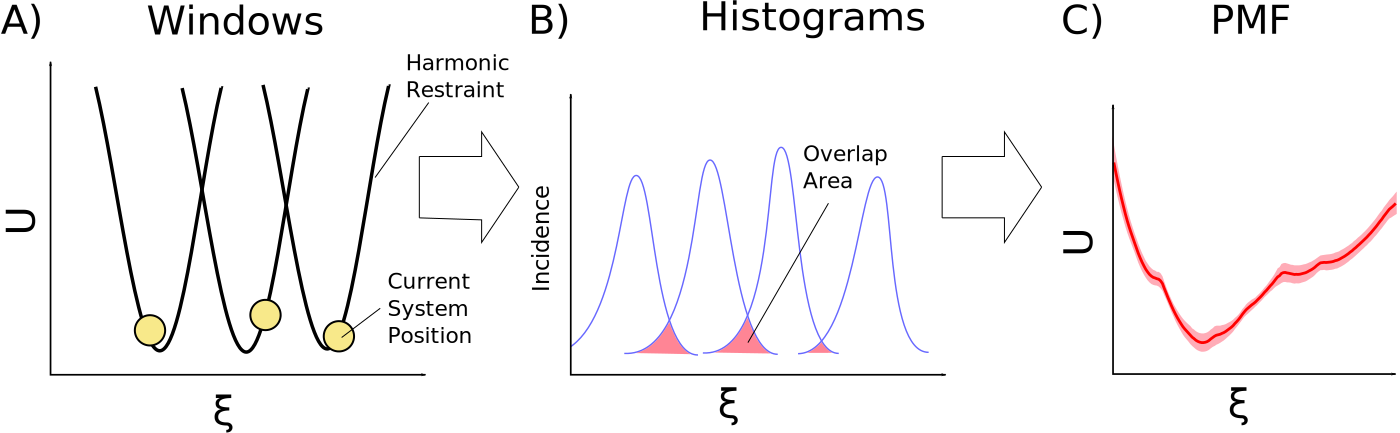
\includegraphics[width=\textwidth]{figures/umbrella_sampling.png.pdf}
	\end{center}
	\captionsetup{singlelinecheck = false, justification=raggedright}
	\caption[Illustration of Umbrella Sampling] {\textbf{Illustration of Umbrella Sampling}}{A) Several simulations are repeated with only one change. A bias  potential is added somewhere along the reaction coordinate $\xi$. B) The value of $\xi$ is recorded in each of the windows and then graphed as histograms. C) The Overlap in neighbouring histograms is integrated via the WHAM method to calculate the Potential of Mean Force. This gives us the energy landscape. Fluctuations in the overlap in the data can be used to estimate the error for the PMF. }
	\label{umbrella_sampling_illustration}
\end{figure}

Umbrella sampling is possibly the most popular method of calculating the free energy of a system along a reaction coordinate. The conceptual philosophy for the method is demonstrated in figure \ref{umbrella_sampling_illustration}. The molecular system is replicated in several ``windows" and a harmonic $U_{biased}$ is added to restrain the collective variable $\xi$ at several different points. The fluctuations of $\xi$ are recorded and the overlap between windows allows us to calculate the potential of mean force (PMF), and thus the energy landscape along the reaction coordinate.  

In more  technical detail, umbrella sampling involves a functional form where $U_{bias}$ separated into $N$ windows. With the bias function in the $n$th window has the form:

\begin{equation}
	U_{b}^n = \frac{k^n_{\xi}}{2}(\xi(\bold{x}) - \xi_0^n)^2
	\label{umbrella_bias}
\end{equation}

Where $\xi_0^n$ is the equilibrium position of the restraint. $k_{\xi}^n$ is the strength of the harmonic restraint in the $n$th window. Typically this is the same in all windows. The more overlap between adjacent windows the more those windows are attracted to each other and the steeper the gradient of the free energy surface (FES) must be pushing those windows together. Conversely, when there is less overlap between adjacent windows it indicates the presence of a barrier in the energy landscape between those windows.

Umbrella sampling is extremely useful for calculating all sorts of experimental quantities and physiologically relevant properties such as folding energies \cite{meshkin2017}, lipid binding \cite{domanski2017}, ion conduction \cite{zhu2012}, and drug binding \cite{subramanian2019}. However, it is particularly sensitive to the choice of initial configuration and collective variable \cite{domanski2017}. The former issue is particular to umbrella sampling because generally short runs are used since so many windows are spawned during the method, the simulations must be at equilibrium \textit{before} the method is attempted, and then sufficient statistics must be collected to average over any conformational changes orthogonal to the collective variable. In these ways, care must be taken when using this method to not introduce systematic error into the calculation \cite{you2019}. A deep knowledge of the molecular system under investigation can help alleviate some of these issues. 

\subsubsection{Weighted Histogram Average Method (WHAM)}
There are a few candidates for calculating a PMF using the statistics calculated in umbrella sampling. The Weighted Histogram Average Method (WHAM) \cite{kumar1992}, Umbrella Integration (UI) \cite{kastner2005} and the Multistate Bennett acceptance ratio (MBAR) \cite{kim2012} are all used. We will briefly outline the mathematical formulation and estimation of errors of the WHAM method as it is more popular \cite{zhu2012}. Our explanation follows \cite{kastner2011} which covers the topic in more detail.

The method begins by dividing the sampled region into a set of $K$ histograms with $K$ being greater than the number of biased windows $N$.  The whole PMF can be estimated (poorly) from the $i$th biased window using 

\begin{equation}
	P_u^i(\xi) = P_b^i(\xi) \exp(\beta U_{b}^i (\xi)) \langle \exp(-\beta U_b^i (\xi))\rangle,
\end{equation}

where the $P(\xi)$  functions represent the probability density function calculated from samples collected at point $\xi$. The samples collected in each histogram then gives us an estimate of the PMF according to equation \ref{unbiased_estimate}. The estimates from each histogram are then combined in a weighted sum using

\begin{equation}
	P_u(\xi) = \sum_i^K p_i(\xi)P_u^i (\xi)
\end{equation}

where the weights, $\sum_{i=0}^N p_j = 1$ are chosen such that the statistical error is minimised across the domain of $\xi$ \cite{chen2011}. This means we solve an optimisation problem for the variance of the unbiased estimates

\begin{equation}
	\frac{\partial\text{Var} (P_u)}{\partial p_i} = 0
\end{equation}

to give the best estimate of the PMF given the samples in each $P_b^i(\xi)$. Essentially we are vertically shifting the estimates obtained in each of the histograms in order to minimise the error across the PMF. 

By convention, we estimate the error in the PMF by splitting up the statistics collected for the distributions of $P^b_i (\xi)$ and constructing PMFs from these independent samples. For example, we might have collected 100 ns of data in each window, but we could construct 5 independent estimates for the PMF using 20 ns blocks of trajectories. The Standard Error of the Mean (SEM) can then be used to estimate the error across the surface \cite{gapsys2020}. By convention, an umbrella sampling calculation is said to have converged when the SEM from these independent samples has fallen below 1 kcal/mol across the PMF. Note that there may be sources of systematic error not captured by this criterion. 

\subsection{Metadynamics}

\begin{figure}
	\begin{center}
		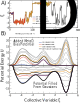
\includegraphics[width=0.7\textwidth]{figures/METAD_demonstration.pdf}
	\end{center}
	\captionsetup{singlelinecheck = false, justification=raggedright}
\caption[Illustration of Metadynamics] {\textbf{Illustration of Metadynamics}}{A) The trajectory of a collective variable $\xi$ in a  metadynamics simulation. The blue region denotes the trajectory up to the time where 20 Gaussians have been deposited. After which the basin at $\xi=0$ has been filled. The red data points denote the time up until 69 Gaussians have been deposited, after which time the second basin at $\xi=-4$ has been adequately sampled. Finally the Orange data indicates that the 3rd basin at $\xi=4$ has been adequately sampled after which which time the system begins to sample $\xi$ diffusively and the simulation has converged. B) The upper panel demonstrates the repulsive potentials that have been added to the simulation in order to drive it to new, unexplored regions. Multiplying the values of this function by $-1$ will be the estimate of the free energy surface\footnote{This is the most simple kind of estimator, used in run of the mill metadynamics but there are more sophisticated estimators for metadynamics variants}. Note how in the lower panel the true potential energy surface is gradually filled by the added Gaussians functions.  Source \cite{bussi2020}}.
	\label{METAD_demonstration}
\end{figure}

Developed in the lab of Michele Parrinello \cite{laio2002}, metadynamics has proven to be a popular method in many applications of computational science, not just in molecular dynamics simulations of biomolecular systems \cite{cheng2017, giberti2015, bussi2020a}. A pedagogical review of the method and its variants written by Pratyush Tiwary can be found in \cite{bussi2020} or by Bussi in \cite{bussi2015}. The method relies on a time dependent form of $U_{bias}$ given by 

\begin{equation}
	U_{bias} (\xi,t) = \sum\limits_{\substack{t' = \tau_D, 2 \tau_D,... \\ t' < t}}  B \ \exp\bigg( - \frac{(\xi(t) - \xi(t') )^2}{2\sigma^2 }\bigg)
\end{equation}

This means that at regular intervals of $\tau_D$ during the simulation we drop virtual, repulsive Gaussian potentials at positions along $\xi$ in order to encourage the simulation to sample regions of $\xi$ it has not visited already. The process is illustrated in figure \ref{METAD_demonstration}. The thermodynamic assumption of this method is that the deposition is done slow enough that the system remains at equilibrium, so a small Gaussian height should be chosen. Usually, the Gaussian widths $\sigma$ are chosen to be the size of the variance in the unbiased measurements of $\xi$. 

The FES estimate at time $t$ from this method is simply the sum of all the Gaussians we have added into the system inverted:  

\begin{equation}
	U_u (\xi,t)  =  \frac{1}{t_c-t} \int_{t_c}^t U_b(\xi,t) dt
\end{equation}

Formally, convergence is reached when the observed probability density is uniform across $\xi$. That is:
\begin{equation}
	P_b (\xi)= \frac{1}{V_\xi } 
	\label{convergence_criterion_metad}
\end{equation}

where $V_\xi$ is the volume of the phase space spanned by $\xi$. However, in practice the function $U_{bias}(\xi)$ is simply inspected at intervals for fluctuations about an average function \cite{sun2016}. 

There are many flavours of metadynamics. The most popular is well-tempered metadynamics which gradually reduces the Gaussian height $B$ as the simulation progresses\cite{barducci2008}. In theory, this guarantees convergence with vanishingly small error. However, this method requires an estimate of how long the simulation will take to converge. There is also infrequent metadynamics which can be used to estimate the diffusion profile along $\xi$ \cite{tiwary2013, tiwary2016, salvalaglio2014, henin2022}.  

A useful feature of the Metadynamics method is that it can be linearly sped up with the number of parallel simulations. This is known as multiple walker metadynamics \cite{raiteri2006}. Since we are simply attempting to sample from the same potential $U_{CHARMM}$ up to a desired time, until the criterion in equation \ref{convergence_criterion_metad} is met, we can speed this process up by running simulations in parallel to sample different regions of $\xi$ and adding Gaussian to the same $U_{bias}$ function.

Conceptually, metadynamics performs the same role as umbrella sampling and should in theory produce the same results in the same system with the same collective variable $\xi$. However, it has some specific contexts where it outperforms umbrella sampling. This method is more suited to an exploration of free energy space where it can intelligently explore regions which are poorly sampled, whereas umbrella sampling requires some foreknowledge of the surface being investigated in order to guess which parts of the landscape require more sampling (in umbrella sampling regions with a high gradient in the FES require a higher density of windows). However, metadynamics can be very difficult to converge. A good indicator of such systematic errors are the presence of unphysically large barriers, indicating that there are orthogonal degrees of freedom not sampled along $\xi$ which might correspond to a minimum energy pathway. These barriers will eventually come down in the infinite sampling limit but many barrier crossings will need to be observed. Excellent discussions of how to solve these systematic errors can be found in articles by Giovanni Bussi \cite{bussi2015, bussi2020a}.

\section{Short Comings of Classical MD}
The short comings of classical molecular dynamics fall into two classes. First is the accuracy of the chemical forcefields outlined in section \ref{forcefields_review}. Second, there is the inability of modern computers to deliver enough samples of the energy landscape to collect sufficient statistics to reach a rigorous conclusion. We are challenged by the physical nature of molecular systems as outlined in section \ref{born-oppenheimer}. The more accurate our forcefields, the more computationally expensive our calculations become, and so the harder it is to deliver a sufficient number of samples. Hence, the solutions to these two problems are diametrically opposed. In the this short section we will explore the current efforts to find solutions to both problems.

\subsection{The Problem with Forcefields}
The approximations inherent in equation \ref{CHARMM_effective_potential_eq} are not without a cost to accuracy. In certain situations, many of which are biologically relevant, it has been shown that polarisation effects not captured by fixed partial charges play an important role in the dynamics of the system. This has been demonstrated in the literature for Gramicidin A, where polarisable forcefields are able to more accurately reproduce the experimental measurements of current \cite{ngo2021}.

The other context where polarisation is important to consider involve divalent ions such as calcium or magnesium. Here, the highly charged environment near a divalent ion will induce changes in the dipole moment of surrounding atoms. This is not possible in the fixed charge formulation in equation \ref{CHARMM_effective_potential_eq}, making investigations of these biologically important chemical species difficult \cite{mamatkulov2013, bergonzo2016}.

However, for most situations, particularly those involving bulk water with a low concentration of solute, classical forcefields are sufficiently accurate to sample conformational motions of biomolecules \cite{hollingsworth2018}. Sadly, it should also be kept in mind that classical MD is not able to simulate any chemistry such as forming and breaking of bonds or a change in the protonation state of an amino acid. Such interactions require considerations of quantum mechanics which are computationally expensive \cite{melo2018}.

There are several efforts to address some of the above issues. Some groups are trying to improve the accuracy of classical forcefields using machine learning and Bayesian inference \cite{nerenberg2018, unke2021}. But there are also attempts to move beyond the functional form of equation \ref{CHARMM_effective_potential_eq} by explicitly including the effects of polarisation. A popular method at the moment is to add a massless drude oscillator as an extra bead to atoms as in the CHARMM drude forcefields, championed by the laboratory of Alexander Mackerell Jr. and others \cite{lin2020}. An alternative solution is to explicitly calculate the dipole and quadrupole moments of each atom at each time step, as is done in the AMOEABA forcefield \cite{shi2013}. These both substantially increase computational cost but have displayed much better agreement with experiments in biological systems, where classical forcefields have been shown to fail \cite{ngo2021, li2017, shi2013}. 

Ultimately, the functional form in equation \ref{CHARMM_effective_potential_eq} used by classical forcefields does not have sufficient degrees of freedom to address all possible chemical contexts. Careful consideration must always be given to whether the forcefield is being used in a faithful way to the situations it was intended to accurately represent. So long as the user is aware of the situations where a given forcefield falls short, classical forcefields can be a powerful tool for the study of molecular systems.

\subsection{The Problem with Sampling}
\label{sampling_problem}

Collecting sufficient statistics about the system of interest is often computationally infeasible in molecular systems. Even though computers have sped up exponentially for the last 50 years we are still orders of magnitude from being able to brute force the time scales of many biological processes, as displayed in table \ref{timescales}.

The slow time step demanded in classical MD due to the fast motions of certain atomic groups such as hydrogen is fundamentally at odds with the time scales of many important biological processes such as drug binding or protein folding which occur on the time scale of milliseconds or seconds.  

Methods are now emerging which can intelligently drive a simulation toward regions unexplored in the collective variable space by unbiased simulations. For some time the field has used steered methods or adaptive sampling methods such as Umbrella Sampling or Metadynamics to drive the simulation toward sections of the energy landscape which are under sampled. These methods universally rely on a choice of collective variable $\xi$ which corresponds to a slow degree of freedom. Such a choice is not usually simple. In the case of ion channels one may rationally choose the placement of the ion along the conduction pathway as the collective variable but the choice is less obvious in the case of more global conformational changes.

The success of simulations at the millisecond timescale by D.E Shaw research suggest that we are in reach of an exciting area in biological research \cite{lindorff-larsen2016, robustelli2022}. Enhanced sampling methods will be able to routinely reach motions that occur on these time scales and as software and hardware improve we will be able to push further, to simulate larger systems. 

The advances we are seeing at the moment which I find exciting are the use of machine learning methods to tease out these degrees of freedom in order to accelerate them with already established enhanced sampling methods. That is, make a more careful choice of the collective variable $\xi$. This could be done with a variety of algorithms such as Principal Component Analysis (PCA) \cite{spiwok2007},\footnote{The use of this collective variable for conformational changes is sometimes called Essential Dynamics.} Time lagged independent component analysis (TICA) \cite{noe2001, schultze2021} from Frank No\"e, a variational approach to conformational dynamics (VACs) from Michelle Parinello's laboratory \cite{brotzakis2019} or Reweighted autoencoded variational Bayes for enhanced sampling (RAVE) \cite{ribeiro2018} from Pratyush Tiwary's laboratory. These algorithms have the potential to build on the above rigorous physics of simulations and revolutionise our understanding of biomolecular systems. As a small example, in chapter \ref{chap:opening} we will discover collective motions using PCA which dilate the CFTR ion channel and study the conduction ions through this dilated structure. 

\section{Conclusion}
It is hoped that the preceding chapter can serve as a roadmap for any physicists interested in beginning to study the exciting field of computational biophysics. The information in each section should serve to help the reader understand the foundations of how simulations are performed. The next steps would be to learn more about the molecular biology and biochemistry of macromolecules so they can better understand the chaotic dance occurring inside cells. For recommended reading on this topic there is Schlick \cite{schlick2010}, Frauenfelder \cite{frauenfelder2010} and Phillips \cite{phillips2012}. There is a lot to learn and the barrier to entry can seem daunting. The reader is encouraged to join mailing lists and other forums where the thriving computational chemistry and computational biophysics communities communicate. Send cold emails asking for help when you are stuck, remember to consult software manuals as well. Below is a list of software to get you started building and running simulations. 

\begin{itemize}
	\item \href{https://www.python.org/about/gettingstarted/}{Python} \cite{van1995python}. A versatile programming language that will help with all parts of a computational workflow.
	\item \href{https://www.ks.uiuc.edu/Research/vmd/}{Visualised Molecular Dynamics} (VMD) \cite{humphrey1996}. Molecular visualisation software with a scripting language, great for building simulation systems, viewing trajectories and rendering figures. 
	\item \href{http://alchemistry.org/wiki/Main_Page}{Alchemistry wiki}. An extensive wiki focussed on pedagogical explanations of alchemical free energy methods. 
	\item \href{https://charmm-gui.org}{CHARMM-GUI} \cite{mallajosyula2015}. A web server which offers a great starting point for constructing MD simulation systems and also offers configuration scripts for all the major MD software packages.
	\item \href{https://www.mdanalysis.org/}{MDANALYSIS} \cite{michaud-agrawal2011, gowers2016}. A python package with a diverse set of tools to analyse molecular dynamics trajectories and structures. 
	\item \href{http://statisticalbiophysicsblog.org/}{Statistical Biophysics Blog} A personal blog by respected computational biophysicist Daniel M. Zuckerman. Here you will find some simple theoretical exercises and some helpful personal advice, not just technical. His book ``Statistical Physics of Biomolecules: An Introduction" is also a very pedagogical introduction to the subject of molecular biophysics.
	\item \href{https://salilab.org/modeller/}{MODELLER} \cite{sali1993, shen2006, webb2016}. A python package which helps build homology models of protein structures or add missing parts to protein models.
	\item \href{https://www.ks.uiuc.edu/Research/namd/}{NAMD} \cite{phillips2005}. A powerful, scalable user friendly MD simulation package.
	\item \href{https://manual.gromacs.org/current/index.html}{GROMACS} \cite{abraham2015}. A less user-friendly MD simulation package than NAMD but offers some different features and (at the time of writing) faster performance.
	\item \href{https://openmm.org/}{OPENMM} \cite{eastman2017}. A flexible MD simulation package that is optimised for usage on GPUs. Is controlled with a python API. A good choice for desktops and workstations.
	\item \href{https://www.plumed.org/}{PLUMED} \cite{tribello2014}. A plugin for existing MD simulation packages which lets the user define their own collective variable $\xi$. Very useful for sophisticated analysis and free energy calculations. 
	\item \href{https://www.rcsb.org/}{Protein Data Bank} (PDB). An open source database of all published biomolecular structures at atomic resolution. 
	\item \href{https://www.uniprot.org/}{Uniprot} \cite{theuniprotconsortium2021}. A database containing a wealth of biochemical data and annotations for proteins, very handy when starting a new project.
	\item \href{https://alphafold.ebi.ac.uk/}{ALPHAFOLD2} \cite{jumper2021}. A highly accurate AI generated database of proteins. This was considered a watershed moment in the field when it was released.
	\item \href{http://mackerell.umaryland.edu/charmm_ff.shtml}{CHARMM forcefield} \cite{huang2016}. The parameter files for the charmm forcefield formatted to be read by popular MD simulation packages.
	\item \href{https://ambermd.org/AmberModels.php}{AMBER forcefield and simulation package} \cite{amber22, ponder2003}. An MD simulation package and toolkit. Here you will also  find instructions for how to extract and use the latest AMBER forcefield in other MD simulation packages.
	\item \href{https://parmed.github.io/ParmEd/html/index.html}{PARMED} \cite{shirts2017}. A python package for converting and manipulating MD file types.
	\item \href{http://www.ccl.net/jobs/} {CCL.net}. A job site where computational chemistry jobs are shared. 
	\item \href{https://www.biophysics.org/} {The Biophysical Society}. The American biophysical society is the largest community of biophysicists. The yearly meetings draw thousands of participants from across the world. At this website you will also find job postings and community news.
\end{itemize}

No individual who has studied a specific discipline has the skills necessary to pick up biomolecular simulation software and begin using it. Physicists lack the understanding of the biology and the chemistry involved in the biological systems, while chemists and biologists may lack an understanding of the deep mathematics that has gone into producing highly accurate simulations of molecular systems. It will take time to get used to an interdisciplinary way of thinking. The reader is also encouraged to seek out collaborators of wet lab disciplines such as cell biologists and protein biochemists to help answer the important problems in biology.

\chapter{Review of Cystic Fibrosis and The Molecular Basis of its Treatment}
\label{chap:cftr}
\chapquote{Because of what's inside me; Because of my genes.}{-Bob Flanagan \cite{dick1997}.}
\newpage
%Authors note:
% We begin with a breif overview of the disease Cystic Fibrosis as it is the main motiation for this project. A horrendous disease for which we will hopefully soon find a cure.

%Clinical outcomes are a chronic illness which affects multiple organ systems and every aspect of a patient's life. 
	%physical therapy, pancreatic sufficiency, ongoing discovery of chronic issues. Much to do. 


% The cause of the disease is CFTR misfunction.
       % CFTR function overview

% CFTR modulators act to restore its function. 
	% patients with rare genotypes cant access modulators.

This thesis primarily focusses on the molecular causes of Cystic Fibrosis (CF). In subsequent chapters we will use Molecular Dynamics (MD) to determine what kind of defect rare mutations cause to the Cystic Fibrosis Transmembrane conductance Regulator (CFTR), the gene whose mutation causes CF. We do this with the goal of understanding what kind of treatments rare disease causing mutations might respond to. Given the importance of the CFTR protein system to this work, we will look at its structure and dynamics in some detail in this chapter. More detail is outlined than is necessary for a simple introduction as I hope this chapter can one day serve as a reference helpful reference text for future endeavours in studying CFTR. However, to understand the motivation for this effort, we will first review some of the medical literature surrounding the disease itself. 

We will first look at some of the symptoms of living with the disease before we look at the structure and function of the CFTR protein---Noting how basic science discoveries and translational research have directly lead to better outcomes for patients. We will then work our way upward to understand the protein system and how it can misfunction and how it can be restored by small molecule drugs. This molecular perspective integrates closely with models based on a patient's own cells which we will use in subsequent chapters to prove that small molecule drugs appear to be capable of treating a diverse set of molecular phenotypes. This is done with the goal of increasing the proportion of patients who can access modulator therapy. 

We will end the chapter with a brief overview of the different experimental techniques which were employed in this thesis to characterise the response of different mutations to different drugs. The language is kept simple in order for the unfamiliar physicist reader to understand some of hte common techniques they will encounter in the literature surrounding biochemistry and cell biology. The intention is not replication but comprehension, so a biochemist familiar with these procedures would likely find the explanations here lacking. The reader is encouraged to at least shadow a lab tech for a day or perform some experiments themselves. Bringing a quantitative mindset to these experiments takes time but is very rewarding.

In previous chapters we always began with the physically smallest scale in order to work upward upward. In chapter \ref{chap:methods} I showed how we can begin from Schr\"odinger's wave equation to understand biomolecular systems. This was to give an example of the philosophy I outlined in chapter \ref{chap:introduction}, taking abstract formalisms and integrating them to model macroscopic biophysical phenomenon. By contrast, in this chapter we will begin with the reality of living with this disease before we look at its molecular cause and its treatment. I have taken particular care to begin this chapter with a discussion of the clinical outcomes of the disease we are studying, so we do not lose sight of our goals in studying biophysics and the reader can appreciate how multifaceted biological problems can be. 

When one trains to practice medicine they are taught how to conduct themselves ethically, with their patients best interests at heart \cite{hajar2017}. I have had no such training and I knew I was missing something by studying this disease so impersonally \cite{foucault1994}. In the 20th century, physicists often participated in political and moral discourse, not always for the better \cite{frank1993, gottfried1999, global2009, rhodes1986, aaronson2008, berger2016, vonneumann_britanica}. Should we wish to embark on the enterprise of studying biophysics we have a responsibility to also study how to do it ethically. Thankfully, many of these important questions have been pondered for some time by philosophers and the reader is encouraged to seek texts on bioethics and also ethics in the use of artificial intelligence \cite{buchanan2000, taneri2011, genome_editting_guildelines_2017, muller2021, bostrom2014}. These considerations will become increasingly important. As biophysics advances, so too does its capacity for misuse \cite{mallapaty2022, urbina2022}. 

%On this somewhat somber note, we will now take a brief look at what it is like to live with Cystic Fibrosis.

%We will then analyse the root cause, mutations to the Cystic Fibrosis transmembrane Conductance Regulator (CFTR). In chapter \ref{chap:conclusion} we will use much of the knowledge gained in this chapter to think about where we can direct future studies to help treat the root cause of Cystic Fibrosis. 



\section{Clinical Realities of Living with Cystic Fibrosis}
Cystic Fibrosis (CF) is the most common fatal genetic condition in Caucasian populations. Over 162 000 people are estimated to be afflicted globally, with a significant proportion living undiagnosed \cite{hammoudeh2021,guo2022}. Even with decades of research there is no known cure for CF patients, who have a life expectancy below 50 \cite{mcbennett2022}. Management of disease symptoms also bears significant financial and emotional costs to patients and their families \cite{vangool2013, page2022}. From a cellular perspective the symptoms of the disease are due to the inability of certain cells to regulate their salt content (Figure \ref{CF_summary}). 

\begin{figure}
	\label{CF_summary}
	\begin{center}
	\includegraphics[width=1\textwidth]{figures/cf_summary_fig.pdf}
	\end{center}
	\captionsetup{singlelinecheck = false, justification=raggedright}
	\caption[Cystic Fibrosis is a Debilitating Disease Whose Cause is Genetic] {\textbf{Cystic Fibrosis is a Debilitating Disease Whose Cause is Genetic}}{Cystic Fibrosis causes misfunction in several major organ systems, affecting all aspects of a patients life. The cause of the disease is genetic, when two defective copies of an anion channel gene, CFTR, are inherited from each parent, epithelial cells cannot pass chloride or bicarbonate ions, leading to a pathogenic buildup of salts inside epithelial cells. In recent decades, small molecule drugs have been discovered which act directly on CFTR to restore its function. This thesis seeks to understand what kind of defects these drugs are capable of rescuing. We find that they are likely to rescue a wide range of defects.} 
\end{figure}

All organs of the body are lined by cells called epithelia. They protect organs from trauma and infection. The most acute symptoms of CF are due to the dehydration of these epithelium in several organs. Of most concern is the epithelium in the lungs. When dehydrated, fine, motile structures called cilia collapse, rendering them unable to ``beat" in order to clear mucus and pathogens \cite{boucher2007, szczesniak2017}. Simultaneously, this dehydration causes the mucus which naturally lines the epithelium to thicken, as osmotic pressure leaches moisture away from it. 

This thickened mucus has two pathogenic effects. Firstly, the stationary mucus allows bacterial colonies to infect the lungs and form a biofilm, this can degrade lung function and remains one of the most troublesome chronic complications in CF patients \cite{chiappini2014}. These infections mean that patients must adhere to strict regimens of antibiotics and avoid other patients in case they expose each other to new or drug resistant pathogens \cite{conway2008}. 

Secondly, and more acutely, the mucus inhibits the normal function of several organ systems. For example, the pancreas is not able to secrete digestive enzymes into the body and the lungs struggle to absorb oxygen. A patient whose pancreas does not produce sufficient enzymes to digest nutrients is referred to as ``pancreatic insufficient" (PI). This is an important determinant in the severity of disease and their quality of life \cite{halloran2011,singh2017}.

As figure \ref{CF_life_expectancy} indicates, much of the increased life expectancy of CF patients has been due to the improved management of this mucus and the populations of bacterium infecting it \cite{mcbennett2022}. Patients often undergo hours of physical therapy each day to help them clear this mucus from their lungs \cite{chest_pt_CFF,thefreylife2015}. Inhalation of a saline solutions may also help relieve symptoms, as this draws moisture out of the epithelial cells by counteracting the pathogenic osmotic pressure gradient \cite{wark2018}. 

In CF care, maintaining lung function remains the primary concern as the organ gradually degrades over the course of the patients life. Respiratory failure is usually the cause of death \cite{kumar2018}. The advent of double lung transplants has lead to a significant increase to the life expectancy of CF patients. However, double lung transplants remain the only option for CF patients as the CF afflicted lung left in their body would infect the donor lung with bacteria \cite{mcbennett2022}. The most common biomarker for tracking disease progress is known as FEV1\%, which stands for Forced Expiratory Volume in 1 second. It is a measure of the volume of air a patient is able to forcibly expel in one second, compared to their total lung capacity \cite{szczesniak2017}. 

CF patients struggle to intake nutrients due to the build up of mucus in the ducts of their pancreas and large intestines. The difficulties associated with nutrition absorption leads to CF related diabetes which afflicts roughly half of adults with CF \cite{Kayani2018}. To manage this complication, patients are often administered digestive enzymes and consume a high fat diet \cite{sullivan2017}. 

Interestingly, as patients are living longer, we are discovering more disease complications, such as bone disorders, meaning there is much clinical work to be done as managing CF becomes a life-long rather than an acute condition \cite{stalvey2013}. Due to the central role CFTR function plays in this disease it will continue to be an important therapeutic target. However, there will also be an increasing need to consider other protein systems, especially due to differential patient responses to modulators \cite{hanafin2021, robertson2015, lingam2017, seelig2020, barbieri2021a, grebert2019}. 

\begin{figure}
	\label{CF_life_expectancy}
	\begin{center}
	\includegraphics[width=0.7\textwidth]{figures/CF_life_expectancy.png}
	\end{center}
	\captionsetup{singlelinecheck = false, justification=raggedright}
	\caption[CF Clinical Progress] {\textbf{CF Clinical Progress}}{The orange line depicts the life expectancy of CF patients in relation to the development of different treatment.  Life expectancy correlates highly with translational research. As CF becomes a chronic condition patients will likely undergo a combination of more and more advanced therapies. Source \cite{garcia2022}} 
\end{figure}


\section{The Misfunction of the CFTR Protein Causes Cystic Fibrosis}

We will now begin our journey upward. Starting by understanding the .

From the perspective of a biophysicist, the cause of Cystic Fibrosis disease is quite simple. The imbalance of salts and water across the epithelium is due to the misfunction of a single gene---an anion channel known as CFTR.

This ion channel is unique. It is a type of protein known as an ABC transporter, designated ABCC7. The ABC super family of proteins bind ATP and use the energy from hydrolysing ATP to pump different substrates across the cell membrane. But CFTR is does not act as a transporter. Rather, it can be thought of as a ``leaky pump" since it still goes through a gating cycle but is incapable of pumping substrate against a concentration gradient \cite{gadsby2006,linsdell2018}. CFTR is an \textit {ion channel}, it allows the passive diffusion of chloride and bicarbonate, but it can also pass larger anions such as glutathione (figure \ref{}) \cite{gadsby2006, tang2009,linsdell1998}. When there is not a sufficient number of functioning channels at the cell membrane, anions cannot pass out of the cell. This causes water to leach through other ion chanels in order to balance this the buildup of osmotic pressure inside the cell \cite{verkman2003}. 

The evolutionary misappropriation of this protein from a transporter into an ion channel is a possible reason for why there are so many mutations which cause it to misfunction \cite{infield2021}.

\subsection{CFTR structure and function}

\begin{figure}
	\begin{center}
	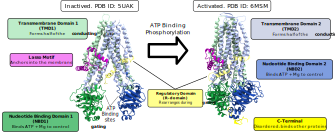
\includegraphics[width=\textwidth]{figures/CFTR_structure.pdf}
	\end{center}
	\label{CFTR_structure_domains}
	\captionsetup{singlelinecheck = false, justification=raggedright}
	\caption[CFTR Structure] {\textbf{CFTR Structure}}{There are currently two resolved human CFTR structures. The inactivated state is neither phosphorylated nor bound to ATP. Observe how the NBDs are far apart and the TMDs are not parallel, forcing a constriction near the top of the protein which does not allow the passage of ions. By contrast, the activated structure is abound to ATP at both sites, bringing the TMDs into a parallel configuration where they are able to form a pore. There are unresolved questions as to whether CFTR may conduct chloride in this conformation which we will analyse in chapter \ref{chap:opening}. All simulations presented in this work were based on the ATP-bound phosphorylated human CFTR structure. PDB ID: 6MSM \cite{zhang2018}.} 

\end{figure}
CFTR is a single chain of 1480 amino acids. The 4 main functional domains have a structure reminiscent of other ABC transporters. There  contains 

CFTR is composed of one chain with pseudo-symmetric structure, the protein is organised into 7 domains \ref{CFTR_structure_domains}. In the order of their primary structure they are: 
\begin{enumerate}
	\item The Lasso motif (AA 1-68), Which anchors into the membrane and serves as an interaction hub with protein partners such as syntaxin and filamin which are important in cellular trafficking \cite{cormet-boyaka2002, naren1998, thelin2007} as well as WNK1 which plays a role in bicarbonate selectivity \cite{kim2019}. 
	\item Transmembrane Domain 1 (TMD1, AA 69-376). This domain forms half of the chloride conducting pore and importantly, TM1 and TM6 in this domain form the extracellular end of the pore for anion permeation \cite{linsdell2006, linsdell2022}. Most positive amino acids which directly interact with anions are located in this domain, even in the inner vestibule \cite{linsdell2018}. We will look at many of these amino acids in detail in chapter \ref{chap:r352q} \cite{wong2022a}. 
	\item Nucleotide Binding Domain 1 (NBD1, AA 377-629). One of the ATP binding sites, this domain has a dense concentration of disease causing mutations, including the most common mutation $\Delta F508$ \cite{cftr2}. This domain contains a Walker A motif but lacks a Walker B motif. This causes one of the ATP binding sites to be degenerate and not allow the hydrolysis of ATP. 

	\item Regulatory Domain (R-domain, AA 630-855). A disordered domain containing up more than 11 known phosphorylation sites \cite{mihalyi2020}. In the inactivated conformation of CFTR, a helical segment of this domain wedges between the TMDs. Binding to PKA encourages this helix to unwedge from between the TMDs, while phosphorylation causes the disordered domain to remain in solution. This process has important consequences for the function of the channel \cite{ostedgaard2000, mihalyi2020}. In the open state, the wedge relocates to a location just below the lasso motif. The identity of the wedge fragment will be analysed in detail in chapter \ref{chap:I37R} \cite{wong2022}. 

	\item Transmembrane Domain 2 (TMD2, AA 856-1168). This domain forms the other half of the chloride conducting pore. There is ongoing controversy over the structure and function of TM8 the function of CFTR \cite{hegedus2022, liu2019}. This helix plays a critical role in regulating channel gating and anion selectivity \cite{negoda2019}.
	\item Nucleotide Binding Domain 2 (NBD2, AA 1169 - 1450). Home to the conserved Q-loop, which regulates the binding of ATP in ABC transporters \cite{ivey2020, zolnerciks2014, dong2015}. This domain contains both a Walker A and a Walker B motif, allowing ATP binding and hydrolysis at one of the sites. 
	\item C-terminus (AA 1451 - 1480). This structure is natively disordered but it serves as an interaction hub in WT-CFTR, anchoring CFTR to other proteins in the cell through its PDZ binding domain \cite{moyer1999, cushing2008}. 

\end{enumerate}


%CFTR is distinguished by a regulatory region known as the R-domain (residues 645-845) which links NBD1 to TMD2. This region acts to lock the channel in the closed state by wedging itself between the TMDs and dislodging when any one of 3 sites are phosphorylated \cite{mihalyi2020}. In experimentally determined structures of human CFTR the secondary structure of a section of the R-domain but not at high enough resolution to determine the identity of individual side chains \cite{zhang2018, zhang2016}. Further secondary structure information can be found through experiments with NMR \cite{Baker2007}.

Previous computational studies of CFTR have used homology models based on the phosphorylated zebra fish protein PDBID:5W81 \cite{zhang2017a} or a distantly related bacterial ABC transporter SAV1866 \cite{dawson2006, Hoffmann2018}. These have yielded interesting results but the sequence similarity between human and zebra fish CFTR is only 55\%. As we will see, CFTR is highly sensitive, its function is poorly conserved under mutations. Note for example how the activity of CFTR correctors is not conserved in mutant zCFTR \cite{laselva2019}.

An open state of the channel has been proposed by combining both the zebra fish homology model and the fully outward facing conformer of the bacterial transporter \cite{Hoffmann2018}. Although this model has several characteristics expected of the open channel, such as the critical R352-D993 salt bridge which we will explore in chapter \ref{chap:R352Q}, it fails to reasonably create a conformation of the selectivity filter which we would expect given biochemical experiments. Additionally, metadynamics studies with the zebrafish channel suggest two extracellular portals which conflicts with experimental studies which indicate only one extracellular portal is present in the human structure \cite{linsdell2018,farkas2020}.


% , it lacks a salt bridge between R104-E116. In experiments, these residues could be replaced by cysteines and the channel would still function. However, when reducing agents were added to the system the channel lost its ability to open fully. This indicates that in the oxidised environment the C104-C116 cysteines formed a disulfide bridge but its breaking upon exposure to reducing agents caused a loss of function in the channel. This indicates that in the WT channel R104-E116 form a stable salt bridge. 

%This salt bridge is clearly visible in the recent cryo-EM structure of ATP-bound human CFTR \cite{zhang2018}.

\subsection{The Gating Cycle}

\begin{figure}
	\begin{center}
	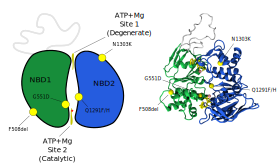
\includegraphics[width=0.8\textwidth]{figures/ATP_head_to_tail_figure.pdf}
	\end{center}
	\label{NBD_structure}
	\captionsetup{singlelinecheck = false, justification=raggedright}
	\caption[NBD Organisation] {\textbf{NBD Organization}}{A) The NBDs are critical to the gating cycle of CFTR. They rest below the TMDs where they bind and hydrolyse ATP in order to regulate the gating cycle. B) Each NBD contacts both ATP molecules. This configuration is known as a head to tail dimer and is common amongst ABC transformers. One of the unique aspects of CFTR is the fact that only one of the ATP binding sites is capable of breaking down its ATP molecule through hydrolysis \cite{stratford2007}. When ATP is hydrolysed at site 2, the channel is allowed to close \cite{infield2021}. The regulatory insertion another unique feature of CFTR and has been shown to increase NBD1 stability when deleted. The  C) Molecular details of how the NBDs bind ATP at the two binding sites. Here we have highlighted several molecular details. The Walker A motifs are on both NBDs and are responsible for stabilising ATP in a conformation which allows hydrolysis to produce ADP and a phosphate group \cite{deltoro2016}. The Walker B motif on NBD2 is directly responsible for mediating hydrolysis, by allowing the movement of the magnesium cofactor \cite{urbatsch2000, rai2006}. Mutation of E1371 in Walker B is sometimes engineered to kill catalytic activity and lock the channel in an open state \cite{stratford2007, zhang2018}. Note the placement of both G551D, a gating mutation and Q1291H/F near site 2. The most common disease causing mutation delF508 is located on a helix of NBD1 which buries itself into a hydrophobic pocket. N1303K is located at a roughly symmetric position on NBD2.   } 

\end{figure}

The conformational transition from inactive to active differs significantly in CFTR compared to other ABC transporters. The NBDs are largely similar to other to those found in other ABC transporters, they dimerise in what is termed a head to tail configuration so both subunits contact both bound ATP molecules \cite{} See FIGURE. Residue E1371 allows nucleophilic attack by surrounding water on the $\gamma$ phosphate  of the ATP bound to Walker B \cite{stratford2007}. The hydrolysis of ATP is the event which causes the channel to gate back to the closed conformation \cite{}. 


Read more: \cite{ramjeesingh1999}

However, the peculiarities arise from the action of the disordered R-domain. In the inactive state this wedges between the TMDs, forming a plug. Intermittently, Protein Kinase A (PKA) will bind one of many segments on the R-domain coaxing the domain into solution. PKA may then phosphorylated a section of the domain, causing to remain in an unplugged configuration.\footnote{Note to physicists, phosphorylation is a process where a phosphate group is added to the side chain of an amino acid. Usually serine, tyrosine or threonine. This phosphate group a charge of -2, wheres these amino acids are normally neutral. This is a key regulator of protein activity as it places a very large charge at a normally neutral site in the protein.}

\subsection {Anion Selectivity}

\begin{figure}
	\begin{center}
	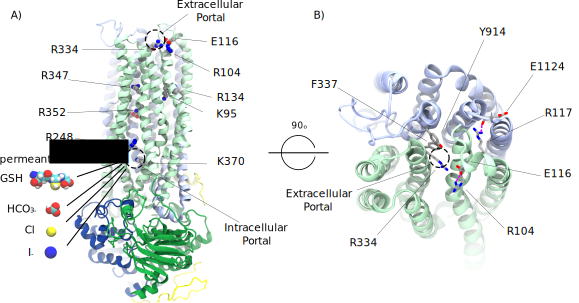
\includegraphics[width=\textwidth]{figures/chloride_passage_figure.pdf}
	\end{center}
	\label{chloride_passage}
	\captionsetup{singlelinecheck = false, justification=raggedright}
	\caption[Chlrodie Passage through CFTR] {\textbf{Chloride Passage Through CFTR}}{A)Ions enter through an intracellular gate, midway through the channel, which is lined with positive amino acids. B) A top down view of the extracellular portal. We have highlighted some hydrophobic amino acids which play important roles in the selectivity of anions. Pictured is the only available structure of the activated human CFTR channel \cite{zhang2018}. Unfortunately, this conformation is not sufficiently open to conduct ions. We will analyse an open conformation in chapter \ref{chap:opening} which we predicted through simulations.} 

\end{figure}
CFTR is weakly selective for specific anions. F337 is the most important amino acid for selectivity, with the F337A mutation leading to a gain of function and a loss in selectivity \cite{wei2016}. Bicarbonate (HCO$_3^-$ is known to have roughly 26\% the permeability of chloride through the channel. Note that Fluoride has even higher conductance through CFTR, likely due to its small size and high solvation energy (does this indicate hydrated conductance?). WNK1 is known to influence the selectivity of the channel https://www.ncbi.nlm.nih.gov/pmc/articles/PMC6889609/. The permeation of bicarbonate is very important physiologically because if a mutation permeates bicarbonate it means there is a high likelihood the patient will be pancreatic sufficient. 

Compared to cation channels like Gramicidin and KcsA, CFTR is only weakly selective, permeating a large set of anions with varying radii and geometries \cite{}. Supposedly it is more permeant to lyotropic (low solvation energy anions) rather than cosmotropic anions (high solvation energy anions) indicating that dehydration of the anion is likely during conductance (CITATION NEEDED). The radius of hydrated chloride ions is 1.7A \cite{yang2002} so even with this larger pore partial dehydration must take place. 

Molecular dynamics studies of the conductance of chloride through the 6MSM structure only saw one extracellular portal. However, they observed multiple pathways between helices. Only 17 conduction events were observed in 10 microseconds of sampling, with a substantial bias of 500mV. This is an order of magnitude less than we would expect for the 0.7 $10^{-12}$S conductance channel. When we consider that the channel must also pass diverse substrates such as bicarbonate, iodide and glutathione, we would expect a more open conformation to exist \cite{kogan2003,linsdell1998}. Such a discrepancy was the basis for the studies in chapter \ref{chap:opening}.


\subsection{Different classes of Cystic Fibrosis Phenotype}
The more than 400 disease causing mutations to CFTR have been classified into 6 common classes based on the nature of the CF they cause, their reaction to CFTR modulators, and results \textit{in vitro} assays. Ultimately I aim to show that at the atomic level there is much more nuance to these and as patient specific theratyping evolves, these classes will become less relevant, serving as illustrative tools only to communicate at a higher level what is going wrong with the CFTR protein. The canonical classification is as follows:

\begin{figure}
	\begin{center}
	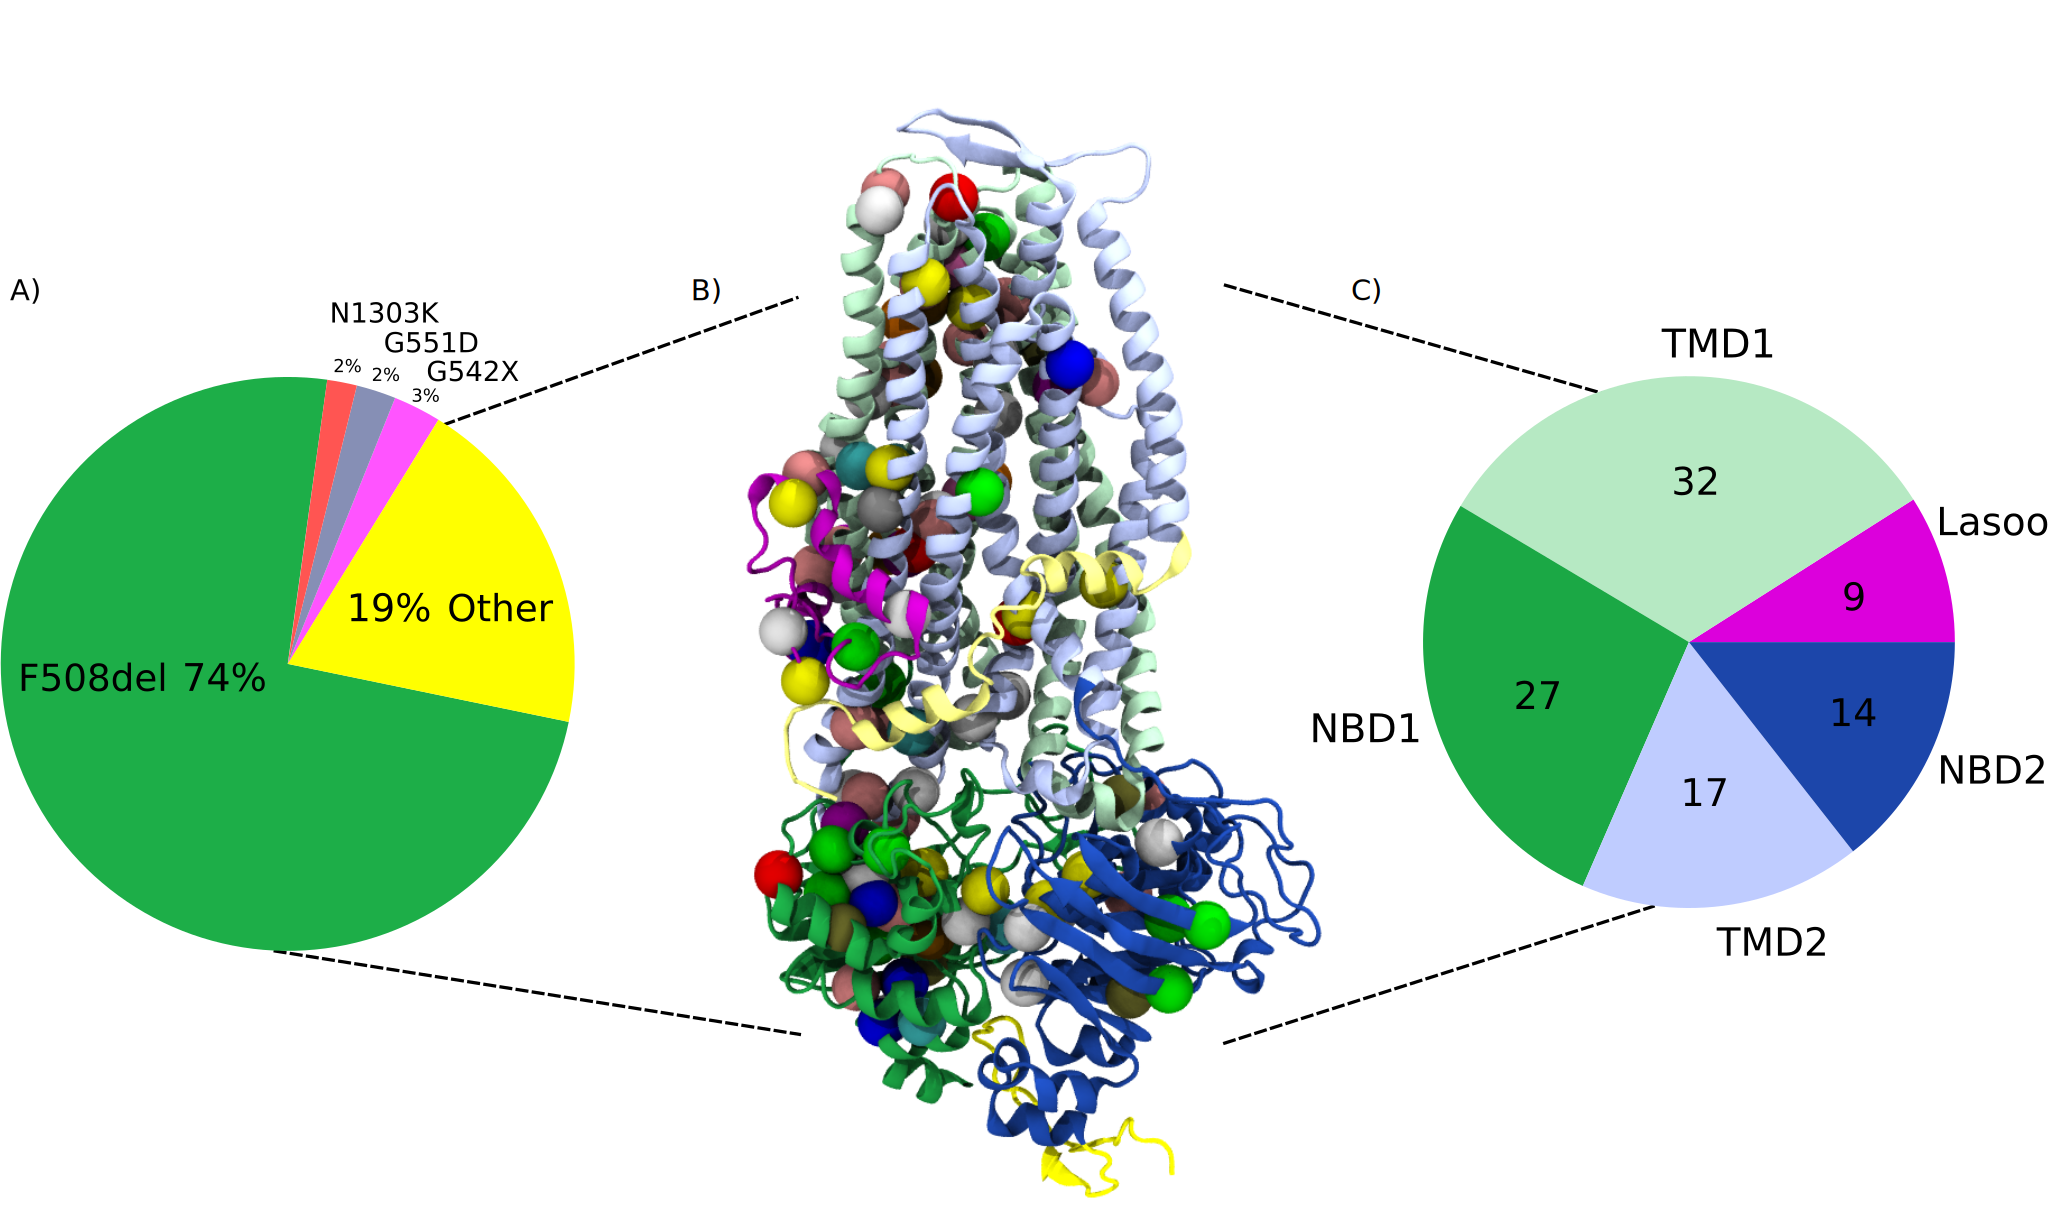
\includegraphics[width=\textwidth]{figures/alleles_pie_chart.pdf}
	\end{center}
	\label{CFTR_structure_domains}
	\captionsetup{singlelinecheck = false, justification=raggedright}
	\caption[Rare Mutations Occur in Across the CFTR Protein] {\textbf{Rare Mutations Occur in All parts of the CFTR Protein}}{A) The reported frequency of all disease causing alleles (not just missense mutations) in the CFTR2 database. At the time of writing there are 402 recorded different disease causing mujtations. A patient with CF will carry two of these mutations. 1 in 25 people of Northern European descent are a carrier for CF and are themselves at increased risk for many health problems \cite{ioannou2014, miller2020}. B) The location of all 112 known disease causing missense mutations mapped on the CFTR protein itself as spheres. In addition to those visualised here there are many of variants of unknown significance (VUS). C) The incidence of CF causing missense mutations in the different domains of the CFTR protein. TMD1 and NBD1 have the highest concentration of disease causing mutations. Likely due to the former's role in ion permeation and the latter's role in gating \cite{cftr2}}. There are no known CF causing missense mutations in the C-terminus or the R-domain. As more patient registries are updated across the world it is likely that more CF causing mutations will be discovered in the future. \footnote{Note that in this figure we have included the novel I37R mutation studied in this thesis. This mutation has not yet been recorded in CFTR2.} 
\end{figure}


\begin{itemize}
	\item \textbf{Class I} No functional protein. Under these mutations no protein is transcribed due to either problems with the transcription of mRNA or a premature stop codon truncating protein synthesis early, meaning the resulting peptide is missing key domains. 
	\item \textbf{Class II} Folding defect. These mutations cause the translated peptide to misfold into the incorrect tertiary structure. This can inhibit the protein's journey as it is trafficked to the cell membrane. 
	\item \textbf{Class III} Impaired Gating. Here the mutation inhibits the ability of the protein to transition from the closed to the open state. 
	\item \textbf{Class IV} Decreased Conductance. These mutations cause a barrier in the energy landscape of the CFTR chloride conductance pathway.
	\item \textbf{Class V} Less Protein Expressed.  
	\item \textbf{Class VI} Decreased Functional Lifetime

\end{itemize}

Although useful, in reality this paradigm does not reflect that a mutation may belong to many categories at once, to differing degrees. In particular in this thesis we will demonstrate that membership of one of these classes can be due to a range of molecular phenotypes. Further, through our molecular simulations we will see that in fact CFTR modulators appear capable of treating many different mutations with unique modes of pathogenesis. We will explain this paradigm in more molecular detail in chapter \ref{chap:conclusions}.

%FIGURE demonstrates how each of the canonical classes at the molecular level is broken down into many sub classes and a mutation might belong to one of many of these subclasses. Structural biology paradigms and \textit{in silico} modelling can help classify mutations into these different classes. In combination with wet lab assays we can understand which classes of these molecular defects are most effectively treated with specific drug regimens. Our computational microscope is helping choose treatments for patients at the atomic level. 

\section{Modulators Act Directly on CFTR to Restore its Function}
Since CF is caused by malfunctions of the channel it makes sense to pursue CFTR as a drug target. Through high throughput \textit{in vitro} screening several four compounds have been developed which act directly on CFTR to rescue its function. These fall into two classes. Correctors, which aid CFTR to fold into the correct state and potentiators which help the channel reach the fully open state once it has folded correctly and integrated into the membrane. Subtleties surrounding the high affinity action of potentiator drugs opens the possibility that specific genetic defects may be optimally rescued by specific combinations and doses of both correctors and potentiators compounds \cite{csanady2019}. Recently, cryo-EM structures of many of these compounds in their bound state have been released \cite{liu2019, fiedorczuk2022}. In addition to several \textit {in vitro} biophysical experiments to determine the precise mechanism of action and binding site of these compounds.

What is remarkable is that modulators they have demonstrated promise in improving not just the most acute symptoms of CF (lung function), but they may be able to treating or even relieve deleterious complications. Modulators have been found to relieve pancreatic insufficiency and CF related diabetes symptoms \cite{gaines2021,lopes-pacheco2020, yi2021} and there is ongoing ongoing study into the possible benefits of modulators on bacterial infections \cite{harvey2022}. This highlights the importance of treating the root cause of a disease like CF.

\subsection{Correctors}
Corrector class modulators are able to treat Class II folding defects. They appear to help the CFTR protein fold into the correct structure by binding to a pocket formed between TM1 and TM3. This hypothesis was generated from circular dichromism \cite{greenfield2006} and fluorescence experiments found that an isolated construct of TMH3 and TMH4 were more likely to fold correctly in the presence of corrector compounds. Later, cryo-EM structures were able to directly image the drugs bound in this location, confirming this hypothesis \cite{fiedorczuk2022}. 

In combination this is strong evidence for the precise mechanism of action for corrector compounds. Further work will aid in the creation of new compounds to refine our exploitation of this mechanism.

\subsection{Potentiators}
Potentiator class drugs bind to CFTR in order to smooth the transition to the fully open, conducting conformation \cite{yeh2017}. This increases the total number of open CFTR ion channels at any one time and helps to balance osmotic pressure over the epithelium.

There is some uncertainty surrounding the precise mechanism of potentiators drugs, with different studies discovering different binding sites via mutagenesis and other methods \cite{yeh2019, liu2019, laselva2021}. Evidence strongly supports their findings that potentiators bind directly directly to CFTR in order to increase the likelihood that it occupies a conducting state, with some potentiators rescuing CFTR with picomolar affinity \cite{csanady2019}. Controversy arises surrounding \textit{where} these drugs are acting to rescue CFTR. There are are cryo-EM structures which show the drugs bound to the TM8 hinge region \cite{liu2019}. However, there are some controversies surrounding the structure in which the drugs are bound in this study which we will discuss in \ref{chap:conclusions}. \textit {In vitro} experiments studying drug binding kinetics suggest at least two membrane facing binding pockets \cite{csanady2019}. 

GLPG1837 has not been approved in a clinical setting. \textit {In vitro} experiments suggest that it is more efficacious even though it has lower affinity for CFTR binding \cite{vanderplas2018}. This would indicate that the highest affinity binding pocket does not produce the greatest modulation. More work is needed to resolve the mechanism which results in the highest clinical effectiveness of these drugs.  

In our work we've found that the atomic nature of the defects introduced by each mutation varies widely, what is interesting is that experiments in \textit{ex vivo} have shown that these drugs are still able to treat this range of different defects. The classification of classes of defect is outdated, really there are as many classes as there are mutations.

\subsection{Read Through Compounds}
Roughly 10\% of mutations result in a premature stop codon in the mRNA of the CFTR gene so synthesis is stopped early. Since there is no full length CFTR protein synthesised by the cells carrying this mutation, potentiators and correctors are unable to directly assist. This has lead to the need to develop a class of drugs known as read through compounds which allow the continued synthesis of the protein past the premature stop codon \cite{sharma2021}. At the time of writing no read through compounds have been clinically approved but efficacy has been demonstrated in pre-clinical models\cite{crawford2021}. Since correctors and potentiators also modulate the behaviour of WT-CFTR it is likely that correctors and potentiators would be given in combination with read through compounds and other therapies as a supplementary treatment.

\section{Patients with Rare Mutations Struggle to Access Modulator Therapy}
CFTR modulators have proven to be a breakthrough in the treatment of CF. However, there is strong motivation behind our focus on rare mutations in this thesis. Roughly 50\% of Cystic Fibrosis cases are caused by a homozygous mutation, $\Delta$F508, and 90\% of patients carry at least one copy of this mutation. At the time of writing, many jurisdictions such as Australia and the EU have approved a triple therapy known as Trikafta which can improve the outcomes for patients with one copy of $\Delta$F508. However, this leaves a significant part of the CF afflicted population without access to this life saving medication, with many more excluded due to the extreme cost of the drugs themselves \cite{administration2021, trikafta_website, abdallah2021, guo2022a}. Clinical studies are also extremely difficult for rare mutations, as there may not be enough patients carrying a specific mutation to study them in the same trial \cite{grody2007}. The work in this thesis demonstrates that a larger section of the CF population is likely to respond to modulators, particularly those carrying missense mutations. Eventually this work will contribute to a practice known as theratyping. An increasingly granular understanding of CF pathogenesis will allow a personalised choice of treatment.

The treatment of rare mutations has particular significance in CF. Not only would patients be otherwise left behind, but by studying rare mutations, outcomes can be improved for all sufferers of CF. For example, potentiator class drugs were discovered by the study of the rare mutation G551D, through high throughput molecular screening \cite{vangoor2009}. By studying rare mutations we can gain a more complete understanding of the nature of the disease and so improve therapies for everybody. This approach will become more important in the future as CF is uncovered in regions where it is rarer, and the population exhibits a broader spectrum of CFTR mutations. Patients in these regions are thus more likely to have a rare form of disease \cite{singh2015,zheng2017,ni2022}. As patient registries are set up in these populations, more rare forms of CF are likely to be discovered \cite{zheng2017}. Considering that patients with the same genotypes often respond differently to the same modulators, it is critical that more modulators are developed, to give all patients more options \cite{hanafin2021}.

%Patients with rare forms of CF are more likely to be in countries where CF is already quite rare \cite{zheng2017}. Patients on modulators have significantly different clinical outcomes even between those with the same genotype. Determining the reason for this would open the door to the development of complimentary therapeutics. 

By explicitly focussing on rare mutations in this thesis we aim to prove that a large subsection of the CF community currently excluded from receiving modulator may in fact to respond to modulators therapy. It would seem that CFTR modulators are capable of treating a wide range of molecular defects. All of the mutations studied in this thesis have a unique mode of pathogenesis but they appear to respond to existing modulators with the same mechanism of action. Such an approach is critical as the earlier patients are able to start modulator therapy the better their prognosis \cite{lahiri2022}. The drugs are well tested in terms of safety and efficacy and now we aim to expand the number of patients who can access modulator therapy \cite{lahiri2022}.

\section{Patient Derived Organoids: A Pre-Clinical Model to Assess Modulators}
Similar to how we took the motions of interacting atoms in chapter \ref{chap:methods} to model a whole protein system, medical researchers seek to would also like to find a model system to study the function of an organ. In CF research, this has lead to the development of techniques where samples of epithelial stem cells from patients the disease are grown into tissues which mimic the function of either the lung or the gut \cite{wong2015,depoel2020}. This is possible in the due to a population of adult stem cells in the epithelium which maintain the ability to differentiate into a variety of cell types (a property known as pluripotency) \cite{blanpain2007}. 

Primarily, these epithelial stem cells are taken from the nasal passages of patients or from rectal biopsies \cite{}. Organoids are excellent model systems, but like all models they are incomplete. They often lack specialized cell types and miss much of the complexity of native organs \cite{clevers2016}. 

Adult stem cells in the epithelium are preferable to other sources of stem cells, as sources which might be easier to harvest would require complex, time consuming protocols to grow into fully developed organoids \cite{wong2012}. Already, the differentiation and expansion of epithelial samples into organoids takes a month \cite{sato2011}.

In the case of CF, this technology allows the construction of a scalable, patient specific platform where a patient's own tissues can be tested to determine the best treatment for them \cite{keegan2021, sato2011}. These pre-clinical models will allow more patients in the heterogeneous set of disease causing mutations to access modulators. This has given rise to an exciting prospect of a practice known as theratyping, enabling clinicians to make a personalised prediction of which therapies will best serve a patient \cite{clancy2019, wong2022, wong2022a, ciciriello2022}. This thesis demonstrates that integration of \textit{in silico} simulations into the process of theratyping can further the capabilities of these pre-clinical models.

%One limitation of these organoid platforms is the lack of an inflammatory response since no immune cells are present in the tissue culture. 
Subsequent chapters will make use of these organoids by testing them with a set of \textit{in vitro} assays in order to characterise a patient's response to modulator therapy, so they are discussed breifly below.

\subsection{Forskolin Induced Swelling to Assess CFTR Function}

\begin{figure}
	\label{western_blot}
	\begin{center}
	\includegraphics[width=1\textwidth]{figures/FIS_demo.pdf}
	\end{center}
	\captionsetup{singlelinecheck = false, justification=raggedright}
	\caption[Forskolin Induced Swelling] {\textbf{Forskolin Induced Swelling}}{Upon exposure to Forskolin, epithelial cells begin to produce cAMP. This causes an increase in intracellular ATP which will open CFTR channels. The influx of water into the cell causes them to swell. The amount of swelling can be used to quantify the amount of properly functioning CFTR in the cell.} 
\end{figure}
Forskolin Induced Swelling (FIS) assays have been used to characterise the patient specific response of a patient's organoids to a drug regimen \cite{dekkers2013}. When epithelial cells are exposed to a chemical known as Forskolin they begin to rapidly produce cyclic AMP (cAMP, a precursor to ATP in a cell) \cite{bonora2012}. The presence of ATP activates the CFTR ion channels, causing the organoids themselves to swell. This swelling allows cell biologists to easily quantify the activity of CFTR within a cell, in a variety of conditions such as the presence of drugs.

\subsection{Electrophysiology Directly Measures CFTR Gating and Conduction}
Since CFTR is an ion channel, measuring its electrical activity is a direct way to assess its function and dynamics. For single channel studies this is done with a patch clamp. However, this does not give an assessment of the whole epithelium. Often the whole organoid is used as a patch and put in an Ussing chamber. By blocking other ion channels such as ENaC during measurements, \footnote{ENaC inhibitors are also being explored as a complimentary therapy to CF modulators\cite{mall2020}.} a clear picture of CFTR function can be measured in order to create a pre-clinical model for a specific patient.

\subsubsection{Ussing Chambers}
An Ussing chambers is a versatile apartaus which allows the measurement of current accross an epithelial membrane. These can be used 

\subsubsection{Patch Clamp Electrophysiology}

\subsection{Western Blotting Assesses CFTR Trafficking}
\begin{figure}
	\label{western_blot}
	\begin{center}
	\includegraphics[width=1\textwidth]{figures/western_blot_explanation.pdf}
	\end{center}
	\captionsetup{singlelinecheck = false, justification=raggedright}
	\caption[Western Blot Explanation] {\textbf{Western Blot Explanation}}{A) Output of a western blot experiment. WT-CFTR has much more abundant protein than delF508 \cite{chang2008}. B) The cell biology behind why the delF508 mutation is pathogenic. When WT-CFTR folds correctly in the Endoplasmic reticulum it is trafficked into the Golgi where it is glycosylated, before it is then implanted into the cell membrane. In the case of delF508, the protein misfolds as it is synthesised, so instead of being trafficked as normal it is prematurely degraded by the proteosome \cite{lopes-pacheco2016a}.} 
\end{figure}
The above methods focus on measuring the electrical activity of the ion channels once they are at the cell membrane, they will only detect functional channels. In order to test the presence of ion channels within the epithelium, functional or otherwise we employ a technique called western blotting. See figure \ref{western_blot} to see how this can help us understand how measure the amount of protein at the cell surface. 

A simplified explanation is given below
\begin{enumerate}
	\item The proteins in the sample are denatured, sometimes by boiling, so they unfold and stretch out into long peptides. 
	\item The proteins in the sample are injected into a gel.
	\item The gel is immersed in a buffer solution and a voltage is applied to it in a process known as electrophoresis. This causes proteins to migrate according to their charge to mass ratio. The larger the protein, the less it will be able to move in the gel. 
	\item The presence of proteins is visualised through immunostaining. First, the gel is washed with a primary antibody. This antibody is specific protein we wish to detect (in our case, CFTR). 
	\item The excess primary antibody is washed off the gel, but some of the antibodies will stay bound to the proteins we are interested in. 
	\item A secondary antibody is washed over the gel. This is engineered to bind to the primary antibody. What is important about the secondary antibody is that it is attached to a special enzyme tag which we can visualise.  
	\item The excess secondary antibody is washed off the gel, but but some of the secondary antibodies will remain bound to the primary antibody.
	\item The tag on the secondary antibody is visualised through the use of chemiluminesence. The tag is typically an enzyme, which emits light when it breaks down a substrate. Hence, for the visualisation step, a photographic film is placed over the gel and it is washed one final time in the substrate of the enzyme which the secondary antibody is attached to. This produces bands in the photographic film, the darker the band is bound at that position, and the more protein is present.
\end{enumerate}
By washing the gel in different  primary antibodies, we can detect multiple proteins in one experiment. This is often used to normalise the amount protein quantity between samples, so you will often see structural proteins such as tubulin or actin in plots. These are used as controls and should not change due to most mutations. Western blotting is thus a simple, widely used technique to quantify the amount of specific proteins in the cell. 

\section{Conclusion}
The combination of the above methods allows us to distinguish between the different classes of mutation which we outlined in section \ref{mutation_classes}. In the next 4 chapters we will make strong use of the these techniques to characterise, in detail, the nature of 4 rare CF causing mutations. This will help us better understand the action of small molecule drugs and how they can be used and developed to treat even more patients.

%=======================================================================================%
\chapter{Molecular Dynamics and Functional Characterization of I37R-CFTR Lasso Mutation Provide Insights into Channel Gating Activity}
\label{chap:I37R}
\chapquote{My name is Benjamin John Goodwin} {-Benjamin John Goodwin (personal communication)}

\section*{\centering Abstract} 

Characterization of I37R, a mutation located in the lasso motif of the CFTR chloride channel, was conducted by theratyping several CFTR modulators from both potentiator and corrector classes. Intestinal current measurements in rectal biopsies, forskolin-induced swelling (FIS) in intestinal organoids, and short circuit current measurements in organoid-derived monolayers from an individual with I37R/F508del CFTR genotype demonstrated that the I37R-CFTR results in a residual function defect amenable to treatment with potentiators and type III, but not type I, correctors. Molecular dynamics of I37R using an extended model of the phosphorylated, ATP-bound human CFTR identified an altered lasso motif conformation which results in an unfavorable strengthening of the interactions between the lasso motif, the regulatory (R) domain, and the transmembrane domain 2 (TMD2). Structural and functional characterization of the I37R-CFTR mutation increases understanding of CFTR channel regulation and provides a potential pathway to expand drug access to CF patients with ultra-rare genotypes.\\

\smallskip

\begin{figure*} [h]
	\begin{center}
		\includegraphics[width=0.80\textwidth]{figures/I37R/graphical_abstract.jpg}
	\end{center}
	\captionsetup{singlelinecheck = false, justification=raggedright}
	\caption[Graphical Abstract. Integration of in silico and in vitro experiments for personalised medicine] {\textbf{Graphical Abstract. Integration of in silico and in vitro experiments for personalised medicine}}{}
	\label{I37R_graphical_abstract}
\end{figure*}

\section{Introduction}
Cystic fibrosis (CF) is a life-limiting genetic disease resulting from mutations in the CF transmembrane conductance regulator (CFTR) gene \cite{ratjen2015}. CFTR—the only member of the ABC transporter family known to be an ion channel—consists of two transmembrane domains (TMD1 and TMD2) which form an anion-selective pore, two highly conserved nucleotide-binding domains (NBD1 and NBD2) with ATP-binding pockets and a newly described N-terminal lasso motif \cite{hwang2013, zhang2016}. In addition, CFTR has a unique, disordered regulatory (R) domain which contains protein kinase A (PKA) phosphorylation sites. For the CFTR channel to open and close (gate), cAMP-dependent PKA phosphorylation of the R domain first activates the CFTR (\cite{gadsby1994}). Then, ATP-binding induces the dimerization of the two NBDs which opens the channel pore and ATP hydrolysis closes the pore.

The lasso motif (amino acids (aa) M1-L69), which is partially embedded in the bilayer and interacts with the R domain, was recently resolved following advancements in cryo-electron microscopy (cryo-EM) of the CFTR structure \cite{liu2017, zhang2018a}. The first 40 amino acids of the lasso motif, which include lasso helix 1 (Lh1, aa V11–R29), form a circular “noose” structure \cite{Hoffmann2018}. The noose structure wraps around the transmembrane helices (TM2, TM6 of TMD1 and TM10, TM11 of TMD2) and is held in place by hydrophobic interactions with L15, F16, F17, T20, L24, and Y28. The C-terminal end of the lasso, which includes the lasso helix 2 (Lh2, aa A46–L61), is tucked under the elbow helix (aa I70–R75) \cite{Hoffmann2018}. Variable disease severity and heterogeneous clinical presentation have been reported for the 78 CFTR variants identified so far in the lasso motif (CFTR1 and CFTR2 databases, Table \ref{chap:I37R}.S1*). Evidently, the lasso motif has a multifunctional role in CFTR regulation with variants impacting folding, gating, and stability of the CFTR protein \cite{fu2001, gene2008, jurkuvenaite2006, sabusap2021, thelin2007}.

CFTR modulators, small molecules which directly target CFTR dysfunction, are now available to certain individuals with CF. Currently, two classes are approved; (1) potentiators, which open the channel pore such as ivacaftor (VX-770) and (2) correctors, which assist CFTR protein folding and delivery to the cell membrane. Type I correctors (lumacaftor/VX-809, tezacaftor/VX-661) stabilize the NBD1-TMD1 and/or NBD1-TMD2 interface by binding directly to TMD1 \cite{loo2013, ren2013} or NBD1 which improves the interaction between NBD1 and the intracellular loops \cite{loo2017, hudson2017}. Type II correctors (C4) stabilize NBD2 and its interface with other CFTR domains while type III correctors (elexacaftor/VX-445) directly stabilize NBD1 \cite{okiyoneda2013}. Combination therapies of corrector(s) and a potentiator (Orkambi, Symdeko/Symkevi, Trikafta/Kaftrio) have been approved for CF individuals with F508del, the most common CFTR mutation, as well as several specific residual function mutations. Most recently, Trikafta/Kaftrio has been approved for patients with a single F508del mutation in combination with a minimal function mutation, broadening the population of patients with CF eligible for treatment with CFTR modulator therapy.

Mounting evidence has shown that in vitro functional studies in patient-derived cell models successfully predict clinical benefit of available CFTR modulators for individuals bearing ultra-rare mutations \cite{berkers2019, mccarthy2018, ramalho2021}. In individuals with CF, adult stem cells are usually collected by taking either airway brushings or rectal biopsies. Single Lgr5+ stem cells, derived from crypts within a patient's intestinal epithelium, can be expanded in culture medium and differentiated into organized multicellular structures complete with the donor patient's genetic mutation(s), thus representing the individual patient \cite{sato2009}. Stem cell models can be used for personalized drug screening to theratype and characterize rare CFTR mutations \cite{awatade2018, berkers2019, pollard2018}. Determining the functional response of rare, uncharacterized CFTR mutations to modulator agents with known CFTR correction mechanisms enables characterization of CFTR structural defects and enhances our understanding of CFTR function.

I37R-CFTR is a novel missense mutation in the lasso motif, detected in an Australian male child diagnosed through newborn screening with elevated immunoreactive trypsinogen, raised sweat chloride ($>$60 mmol/L), and CFTR Sanger sequencing identifying c.1521-1523del (F508del) and c.110C $>$ T (I37R) mutations (Table \ref{chap:I37R}.S2*). We used functional studies and molecular dynamics (MD) simulations to characterize the functional and structural defects of I37R-CFTR. CFTR function was assessed using intestinal current measurements (ICM) in rectal biopsies, forskolin-induced swelling (FIS) assays in intestinal organoids, and short circuit current measurements (Isc) in I37R/F508del organoid-derived monolayers, respectively. The potentiators VX-770 (approved), GLPG1837 (phase II clinical trials), and genistein (a natural food component with potentiator activity \cite{dey2016}) were tested as monotherapies, dual potentiator therapies, or in combination with correctors (VX-809, VX-661, and VX-445). We compared this to our laboratory reference intestinal organoids. For MD simulations, we modeled and examined the structural defect of the I37R mutation on an extended cryo-EM structure of ATP-bound, phosphorylated human CFTR (PDB ID code 6MSM) \cite{zhang2018a}.

\section{Results}
\subsection{I37R-CFTR Baseline Activity in Patient-Derived Rectal Biopsies and Intestinal Organoids}
Intestinal current measurements (ICM) were performed on I37R/F508del and reference CF (F508del/F508del, G551D/F508del) and non-CF (wild-type: WT/WT) rectal biopsies using a standard protocol \cite{clancy2013, graeber2015} (Figure \ref{I37R_figure1}A). Following stimulation with a forskolin (fsk) and IBMX cocktail, rectal biopsies from the I37R/F508del CF participant elicited cAMP-dependent currents of 45.8 ± 3.8 $\mu$A/cm$^2$—an appreciable 50\% of WT-CFTR activity (p $<$ 0.05; Figure \ref{rectal_organoids_1}A, Table \ref{chap:I37R}.S3*). This response was at least 4-fold higher than those of the reference CF biopsies, although statistical significance was not reached.

%\noindent

\begin{figure}
\begin{center}
\includegraphics[width=\textwidth]{figures/I37R/rectal_organoids.jpg}
\label{I37R_figure1}
\end{center}
%\captionsetup{singlelinecheck = false, justification=raggedright}
\begingroup
\captionof{figure}[Characterization of I37R-CFTR residual function in rectal biopsies and intestinal organoids]{\textbf{Characterization of I37R-CFTR residual function in rectal biopsies and intestinal organoids}}{
(A) Representative Ussing chamber recordings of intestinal current measurements (ICM) in rectal biopsies from WT-CFTR control participants and participants with CF. Dot plots of cAMP-induced current ($\Delta$Isc-Fsk + IBMX) in participants with WT/WT (n = 2), F508del/F508del (n = 3), G551D/F508del (n = 1), and I37R/F508del (n = 1) CFTR genotypes. Experiments were performed in the presence of 10 $\mu$M indomethacin. Arrows indicate the addition of compounds: 100 $\mu$M apical amiloride (1. Amil), apical and basal addition of 10 $\mu$M forskolin +100 $\mu$M IBMX cocktail (2.Fsk + IBMX), 100 $\mu$M basal carbachol (3.CCh), and 100 $\mu$M basal bumetanide (4.Bumet). The Isc at the time CCh was added (middle horizontal dotted line), and the maximum (top dotted lines) and minimum (bottom dotted lines) Isc induced are indicated. Each dot represents an individual replicate.\\

(B) Immunofluorescence staining of CFTR (green), e-cadherin (red), and DAPI (blue) in a rectal biopsy derived from an I37R/F508del participant. 63x/1.4 oil immersion objective. Scale bar = 50 $\mu$m.\\

(C) Immunofluorescence staining of e-cadherin (green), Ki67 (red), and DAPI (blue) in intestinal organoids derived from an I37R/F508del participant. 20x/0.75 dry objective. Scale bar = 100 $\mu$m.\\

(D) Western blot in WT/WT, F508del/F508del, and I37R/F508del intestinal organoids. CFTR maturation was calculated by measuring the level of mature mutant CFTR (Band C) as a percentage of mature CFTR from WT organoids (\% normal CFTR). All data were normalized to the calnexin loading control. B and C represents the mature, complex-glycosylated CFTR. B and B represents the immature, core-glycosylated CFTR. See Figure \ref{chap:I37R}.S9* for uncropped Western blot images.\\

(E and F) Forskolin-induced swelling (FIS) assay in organoids from participants with F508del/F508del (n = 5), G551D/F508del (n = 2), and I37R/F508del (n = 1) CFTR genotypes. Organoids were stimulated with forskolin (fsk) concentrations ranging from 0.02 to 5 $\mu$M.(E) FIS expressed as the means ± standard deviation (SD) of the area under the curve (AUC) calculated from t = 0 (baseline) to t = 60.(F) FIS of organoids at 0.8$\mu$M fsk at baseline represent residual CFTR function. Data represented as violin plots with mean to show distribution.\\

(G) Immunofluorescence staining of e-cadherin (green), ZO-1 (red), and DAPI (blue) in organoid-derived monolayers from a CF participant. 20x/0.75 dry objective. Scale bars = 50 $\mu$m.\\

(H) Representative Ussing chamber recordings of short circuit current in organoid-derived monolayers from a WT-CFTR control participant and participants with CF. Dot plots of fsk-induced current ($\Delta$Isc-Fsk) in participants with WT/WT (n = 1), F508del/F508del (n = 1), and I37R/F508del (n = 1) CFTR genotypes. Experiments were performed in the presence of 10 $\mu$M indomethacin. Arrows indicate the addition of compounds: 100 $\mu$M apical amiloride, 5 $\mu$M basal fsk, 30 $\mu$M apical CFTR inhibitor CFTRinh-172, and 100 $\mu$M apical ATP. Each dot represents an individual replicate. Data in (A) and (H) represented as mean ± standard error of the mean (SEM). One-way analysis of variance (ANOVA) was used to determine statistical differences. * p $<$ 0.05, ** p $<$ 0.01, **** p $<$ 0.0001.\\
}
\endgroup
\end{figure}

\smallskip

Co-activation with carbachol (CCh) resulted in a biphasic response in the I37R/F508del biopsies, characteristic of residual CFTR chloride channel function in the CF colon \cite{graeber2015,veeze1994}. The initial negative Isc peak indicates apical potassium secretion reached 9.4 ± 2.5 $\mu$A/cm$^2$. Following this, the CCh-induced positive Isc indicates the increase of apical chloride secretion reached 15.78 ± 2.07 $\mu$A/cm$^2$. This biphasic response was similarly observed in the G551D/F508del biopsies (25.77 ± 2.16 $\mu$A/cm$^2$) but was diminished in the F508del/F508del biopsies (−2.28 ± 1.65 $\mu$A/cm$^2$). These findings are in accordance with the localization of CFTR protein at the plasma membrane (mature complex-glycosylated CFTR) of the I37R/F508del rectal biopsies, as demonstrated by immunofluorescence staining (green; Figure \ref{I37R_figure1}B).

Next, CFTR protein expression and maturation was assessed in I37R/F508del, reference F508del/F508del, and WT/WT organoids using Western blot (Figures \ref{I37R_figure1}C-D). The expression of complex-glycosylated C band in I37R/F508del organoids was 23.7\% that of the WT/WT organoids, considerably higher than the 6.4\% detected from F508del/F508del organoids (Figure \ref{I37R_figure1}D). CFTR activity was then evaluated in I37R/F508del and CF reference intestinal organoids using a fsk-induced swelling (FIS) assay at four fsk concentrations between 0.02 and 5 $\mu$M (Figure \ref{I37R_figure1}E). FIS of I37R/F508del intestinal organoids at 0.8 $\mu$M fsk—the optimal concentration for baseline assessment of CFTR activity \cite{dekkers2016}—was 282.9 ± 36.0 (Figures \ref{I37R_figure1}E-F). This exceeded the baseline FIS of the reference intestinal organoids by at least 7-fold (F508del/F508del: AUC = 42.8 ± 19.4; G551D/F508del: AUC = 21.3 ± 29.4).

The morphological difference between WT (pre-swollen) and CF organoids \cite{cuyx2021}, means comparing CFTR activity between CF and healthy CFTR function by FIS assay cannot be achieved \cite{dekkers2016,vanmourik2019}. In order to compare I37R/F508del to wild-type CFTR activity, organoid-derived monolayers were created (Figure \ref{I37R_figure1}G) and CFTR ion transport was performed \cite{zomer-vanommen2018}. Fsk-stimulated CFTR-dependent currents were 9-fold higher in I37R/F508del monolayers than those of reference F508del/F508del monolayers (7.3 ± 0.2 vs 0.8 ± 0.1 $\mu$A/cm$^2$; p $<$ 0.0001), but 12-fold lower than WT/WT monolayers (87.5 ± 1.3 $\mu$A/cm$^2$; p $<$ 0.0001) (Figure \ref{I37R_figure1}H). This is consistent with the FIS assay results demonstrating high baseline CFTR activity in I37R/F508del intestinal organoids.

\subsection{I37R-CFTR Functional Response to CFTR Modulator Monotherapy in Intestinal Organoids}

We investigated the functional response of I37R/F508del organoids to single potentiators: VX-770, GLPG1837 (G1837), and genistein (Gen). Treatment with VX-770 minimally increased FIS of I37R/F508del organoids by AUC of 59.7 above baseline at 0.128 $\mu$M fsk (Figures \ref{I37R_figure2}A–C and \ref{chap:I37R}.S1*)—the optimal concentration for in vitro assessment of CFTR modulator response to predict clinical effect \cite{dekkers2016}. G1837 and Gen both significantly increased FIS, albeit with different efficacies (655.8 and 256.8, respectively; Figures \ref{I37R_figure2}A–C and \ref{chap:I37R}.S1*). None of the potentiator treatments increased FIS in F508del/F508del organoids, indicating no improvement in CFTR activity in response to potentiator therapy (Figure \ref{I37R_figure2}C). Only G1837 significantly increased FIS in the G551D/F508del organoids (210.4 ± 57.5; p $<$ 0.01). In comparison to G551D/F508del organoids, G1837 was 3-fold more efficacious in the I37R/F508del organoids (p $<$ 0.0001).


testing


\begin{figure}
\begin{center}
\includegraphics[width=\textwidth]{figures/I37R/rectal_organoids_response.jpg}
\label{I37R_figure2}
\end{center}
\begingroup
\captionof{figure}[Characterization of I37R-CFTR functional response to corrector or potentiator monotherapy in intestinal organoids]{\textbf{Characterization of I37R-CFTR functional response to corrector or potentiator monotherapy in intestinal organoids}}{
Forskolin-induced swelling (FIS) assay in organoids from participants with F508del/F508del (n = 5), G551D/F508del (n = 2), and I37R/F508del (n = 1) CFTR genotypes. Organoids were incubated overnight with 0.03\% DMSO (untreated) or 3 $\mu$M VX-809 or 3 $\mu$M VX-661 or 3 $\mu$M VX-445. After 24 h, organoids were stimulated with fsk concentrations ranging from 0.02 to 5 $\mu$M, either alone or in combination with potentiator monotherapy (3 $\mu$M VX-770 or 3 $\mu$M G1837 or 50 $\mu$M Gen).\\

(A) FIS of I37R/F508del organoids stimulated with VX-770, GLPG1837 (G1837), or genistein (Gen) monotherapy, expressed as the means ± standard deviation (SD) of the area under the curve (AUC) calculated from t = 0 (baseline) to t = 60 min.\\

(B) Representative brightfield images of I37R/F508del organoids at baseline (t = 0) and after 1 h of stimulation (t = 60) at 0.128 $\mu$M fsk. Scale bars = 100 $\mu$m.\\

(C) FIS of organoids at 0.128$\mu$M fsk following stimulation with VX-770, GLPG1837 (G1837), or genistein (Gen) monotherapy. Data corrected for baseline FIS and represented as violin plots with mean to show distribution.\\

(D) Representative Ussing chamber recordings of short circuit current in I37R/F508del organoid-derived monolayers. Dot plots of total currents stimulated by DMSO or G1837 plus fsk. Experiments were performed in the presence of 10 M indomethacin. Arrows indicate the addition of compounds: 100 M apical amiloride, apical addition of either vehicle control 0.01\% DMSO or 10 $\mu$M G1837, 5 $\mu$M basal fsk, 30 $\mu$M apical CFTR inhibitor CFTRinh-172, and 100 $\mu$M apical ATP. Each dot represents an individual replicate. Data represented as mean ± standard error of the mean (SEM).\\

(E) FIS of I37R/F508del organoids pre-incubated with corrector (VX-809 or VX-661 or VX-445) for 24 h, expressed as the means ± standard deviation (SD) of the area under the curve (AUC) calculated from t = 0 (baseline) to t = 60 min.\\

(F) Representative brightfield images of I37R/F508del organoids at baseline (t = 0) and after 1 h of stimulation (t = 60) at 0.128 $\mu$M fsk. Scale bars = 100 $\mu$m.\\

(G) FIS of organoids at 0.128$\mu$M fsk following incubation with corrector (VX-809 or VX-661 or VX-445) for 24 h. Data corrected for baseline FIS and represented as violin plots with mean to show distribution. One-way analysis of variance (ANOVA) was used to determine statistical differences except in (D) where unpaired t test was used. **p $<$ 0.01, ***p $<$ 0.001, and ****p $<$ 0.0001. aP for G1837, bP for Gen and cP for VX-445 of I37R/F508del, \^P for G1837 vs VX-770, or Gen and \#P for VX-445 vs VX-809 or VX-661.\\
}
\endgroup
\end{figure}

Because G1837 demonstrated the greatest restoration of CFTR activity in I37R/F508del organoids, we evaluated G1837 treatment of I37R/F508del organoid-derived monolayers. G1837 led to a significant 1.5-fold increase in fsk-stimulated currents ($\Delta$Isc: 4.4 $\mu$A/cm$^2$; p $<$ 0.0001) (Figure \ref{I37R_figure2}D). This is consistent with the FIS of I37R/F508del organoids, indicating that I37R-CFTR responds to potentiator agents.

Given the I37R/F508del high residual CFTR activity and its localization at the epithelial cell surface, we hypothesized that the I37R-CFTR mutation has minimal impact on CFTR protein folding or maturation. Treatment of I37R/F508del organoids with type I corrector agents (VX-809 or VX-661) did not significantly increase FIS above baseline (Figures \ref{I37R_figure2}E–G and \ref{chap:I37R}.S1*). In contrast, treatment of I37R/F508del organoids with a type III corrector agent (VX-445) significantly increased FIS by AUC of 1112.5 above baseline, greater than those in the F508del/F508del organoids (42.5). VX-445 has been shown to act as both a corrector and potentiator for certain CFTR mutations \cite{laselva2021,shaughnessy2021,veit2021}. Acute treatment of I37R/F508del organoids with VX-445 did not improve potentiation of CFTR (Figure \ref{chap:I37R}.S1*). This supports the observation that VX-445-stimulated rescue of CFTR in I37R/F508del organoids acts by a correction mechanism improving I37R mild folding and processing defects. I37R-CFTR functional response to CFTR modulator co-therapies in intestinal organoids.

Combination treatments of CFTR modulators are used to treat patients bearing CFTR mutations with multiple functional defects such as F508del and patients who are heterozygous for CFTR mutations. We investigated the effect of combinations of potentiators. Dual potentiator combinations increased FIS of I37R/F508del organoids to a greater extent than the respective single potentiators (Figure \ref{I37R_figure3}A) and had a synergistic effect, where the FIS was greater than the sum of the respective single potentiators (Table \ref{chap:I37R}.S4*). Despite G1837 + Gen having greater efficacy than the other dual potentiator combinations, the magnitude of response was not statistically different between the different combinations of dual potentiators (Figure \ref{I37R_figure3}A).

Co-therapy with a corrector (VX-809 or VX-661) and dual potentiators significantly (p $<$ 0.01) increased FIS of I37R/F508del organoids compared to co-therapy of a corrector with VX-770 or Gen, but not G1837 (Figure \ref{I37R_figure3}B). VX-809/G1837 + Gen co-therapy had the greatest efficacy, increasing FIS 1904.0 above baseline. In contrast, corrector/VX-770 + Gen co-therapy had the least efficacy. This trend was consistent with that of the dual potentiators synergistic effect.

Dual correctors (VX-445+VX-661) increased FIS in I37R/F508del organoids by AUC of 1856.6 above baseline, which corresponds with the level of rescue achieved by the most effective corrector/dual potentiator co-therapy (VX-809/G1837 + Gen). The triple combination therapy with dual correctors and a potentiator further increased FIS in I37R/F508del organoids by AUC of 3101.6 above baseline. It is therefore the most effective modulator combination tested in this study.

\begin{figure}
\begin{center}
\includegraphics[width=\textwidth]{figures/I37R/rectal_organoids_triple_therapy.jpg}
\label{I37R_figure3}
\end{center}
\begingroup
\captionof{figure}[Characterization of I37R-CFTR functional response to dual potentiator or corrector therapy or corrector(s)-potentiator(s) co-therapy in intestinal organoids]{\textbf{Characterization of I37R-CFTR functional response to dual potentiator or corrector therapy or corrector(s)-potentiator(s) co-therapy in intestinal organoids}}{
	Forskolin-induced swelling (FIS) assay in organoids from participants with F508del/F508del (n = 5), G551D/F508del (n = 2), and I37R/F508del (n = 1) CFTR genotypes.\\

	(A and B) Organoids were incubated overnight with 0.03\% DMSO (untreated) or 3 $\mu$M VX-809 or 3 $\mu$M VX-661 or 3 $\mu$M VX-445 + 18 $\mu$M VX-661. After 24 h, organoids were stimulated with fsk ranging in concentration from 0.02 to 5 $\mu$M, either alone or in combination with a single potentiator (3 $\mu$M VX-770 or 3 $\mu$M G1837 or 50 $\mu$M Gen) or dual potentiators (VX-770 + G1837 or VX-770 + Gen or G1837 + Gen). FIS of organoids at 0.128$\mu$M fsk stimulated with VX-770, GLPG1837 (G1837), or genistein (Gen) or their combinations, following (A) 24 h pre-incubation with DMSO (untreated) or (B) corrector (VX-809 or VX-661), respectively.\\

	(C) FIS of organoids at 0.128$\mu$M fsk stimulated without or with VX-770, following 24 h pre-incubation with dual correctors (VX-445+VX-661). Data corrected for baseline FIS and represented as violin plots with mean to show distribution. One-way analysis of variance (ANOVA) was used to determine statistical differences except in (C) where unpaired t test was used. *p $<$ 0.05, ***p $<$ 0.001, ****p $<$ 0.0001
}
\endgroup
\end{figure}

\subsection{I37R-CFTR Perturbs the Noose Structure of the Lasso Motif}

We next characterized the structural defect of I37R-CFTR using MD simulations. The primary structure of the lasso motif (M1-L69) is conserved across 230 vertebrate species (Figure \ref{chap:I37R}.S2, Table \ref{I37R_S5}). The lasso motif formed a noose structure that rested against TMD2 (Figure \ref{I37R_figure4}A). Amino acids V12-R29 were embedded in the plasma membrane while the rest of the lasso motif resided in the cytosol. The noose structure was maintained by a salt bridge formed between K26 and D36 (Figure \ref{I37R_figure4}B). I37 was positioned in the center of this noose, within a hydrophobic pocket formed by amino acids from the lasso, TMD2, and the poorly resolved R domain in the cytosol (Figure \ref{I37R_figure4}C).

\begin{figure}
\begin{center}
\includegraphics[width=\textwidth]{figures/I37R/MD_cftr.jpg}
\label{I37R_figure4}
\end{center}
\begingroup
\captionof{figure}[Placement of I37R within the lasso motif and the resulting changes to its conformation]{\textbf{Placement of I37R within the lasso motif and the resulting changes to its conformation}}{
	(A) Ribbon structure of human CFTR, partially embedded within the plasma membrane (gray surface). I37 rendered as spheres. TMD: transmembrane domain; NBD: nucleotide-binding domain; R: regulatory domain (R domain).\\

	(B) K26-D36 salt bridge stabilizing the noose structure of the lasso motif. Charged amino acids depicted as balls and sticks. I37 rendered as spheres, and color-coded by element (gray: C; white: H; red: O; blue: N).\\

	(C) I37 positioned within a hydrophobic pocket formed by amino acids from the lasso motif, TMD2, and poorly resolved R domain. Relevant amino acids labeled and depicted as spheres in TMD2, and as balls and sticks in lasso motif and R domain.\\

	(D) Residue-wise root-mean-square deviation (RMSD) to the C-alpha atoms of the WT-CFTR 6MSM model, measuring the conformational change of the WT (pink) and I37R mutant (orange) lasso after 2 $\mu$s simulations. Values are means sampled over the last $\mu$s of simulations.\\
}
\endgroup
\end{figure}

Mutation of the evolutionarily conserved, non-polar and uncharged isoleucine (I) of I37 to a positively charged arginine (R) introduced an unstable lone charge into the hydrophobic pocket within the lasso motif noose. We hypothesized that this likely results in the rotation of the R37 side chain out of the hydrophobic pocket, and possible coordination with negative charges in the nearby R domain.

To identify a reasonable conformation of the mutant lasso motif, the WT 6MSM model was mutated to R37 and three 2 $\mu$s simulations were performed at physiological temperature (310 K). The R37 side chain rotated out of the hydrophobic pocket in only one of the three simulations. The difference between the root-mean-square deviation (RMSD) of the noose structure of I37R-CFTR compared to the WT was on average 2.8 $\mbox{\AA}$ at the amino acids M1-L6, and 1.8 $\mbox{\AA}$ at L34-S50 (Figure \ref{I37R_figure4}D). To confirm this observation, repeat simulations were performed at 350 K (40$^\circ$C above physiological temperature), a temperature shown to accelerate the potential conformational transitions of proteins \cite{beckerman2015}. In these higher temperature simulations, the root-mean-square fluctuation (RMSF) of the region around amino acid 37 doubled in two out of three simulations, compared to WT-CFTR at 310K (Figure \ref{I37R_S3}). This confirmed the destabilization of the lasso motif by I37R-CFTR. All WT-CFTR domains and the surrounding bilayer remained stable at the elevated temperature (Figures \ref{I37R_S4} and \ref{I37R_S5}).

\subsection{I37R Mutation Strengthens Lasso Motif Interaction with the R-domain}

In the 6MSM structure, the R domain is largely unresolved with two exceptions: the first (Q637) and last (T845) amino acids that adjoin neighboring domains, and the backbone atoms of a 17 amino acid segment. This latter segment consists of an eight amino acid disordered coil followed by a nine amino acid alpha-helix \cite{zhang2018a}. The alpha-helix was separated by approximately 10$\mbox{\AA}$ (1 nm) minimum C-alpha distance to I37 in the lasso motif. This suggested a likely interaction between this segment of the R domain and I37, which necessitated partial modeling of the R domain (Figure \ref{I37R_figure5}A).

\begin{figure}
\begin{center}
\includegraphics[width=\textwidth]{figures/I37R/MD_cftr_2.jpg}
\end{center}
\begingroup
\captionof{figure}[I37R interacts with a previously unresolved section of the R domain]{\textbf{I37R interacts with a previously unresolved section of the R domain}}{
	(A) The reconstructed R domain amino acids (yellow), depicting the assignment of L818-F834 to the 17 amino acids with only the backbone resolved in the 6MSM structure, and the linking residues to T845 in TMD2. Lasso motif in purple. Side chains depicted as balls and sticks.\\

	(B) The stabilities of all 24 modeled R domain assignments, quantified by RMSD to the 6MSM structure. The most stable alignment of the 17 unidentified amino acids, L818-F834, is highlighted yellow. The full list of tested assignments is shown in Supplementary material 9*.\\

	(C) The minimum N-O distance between newly formed and disrupted salt bridges in the I37R mutant. Distance less than 4 Å indicates direct contact. Values are means ± standard deviations (SD), sampled over the last 500 ns of simulations.\\

	(D) Conformational changes in the I37R mutant (orange) compared to WT (purple) lasso motif, which brings it closer to the R domain (yellow). Minimum C-alpha atom distance between amino acid 37 and the R domain helix (E826-F834) in I37R and WT.
}
\label{I37R_figure5}

\endgroup
\end{figure}

Modeling of these 17 unidentified amino acids was performed by creating 24 different in silico models of this segment based on the 6MSM structure. In each model, a unique 17 amino acid sequence was determined with a sliding window of one amino acid, starting backwards from amino acid T842 due to the alpha-helix’s 20 $\mbox{\AA}$ proximity to T845. The 17 amino acids were then connected to T845 with the missing linking amino acids. The structural stability of all 24 modeled segments was tested by performing up to 300 ns simulations for each model and comparing the backbone RMSD measurements against 6MSM (Figures \ref{I37R_figure5}B and \ref{I37R_S6}). The model with the lowest RMSD (3 $\mbox{\AA}$) and thus the highest stability was attained when L818-F834 was assigned to the unidentified 17 amino acids, of which the alpha-helix maps to E826-F834 (Figures \ref{I37R_figure5}B and \ref{I37R_S6}). This assignment was corroborated by NMR measurements of the isolated R domain in solution, where the same segment retained partial helicity \cite{baker2007}. Predictions of the structure of human CFTR by Alphafold2 also aligned with this assignment of primary structure to the unidentified amino acids (Figure \ref{I37R_S7}) \cite{jumper2021}. Several favorable interactions between this R domain model and other parts of the CFTR protein further supported this assignment (Figures \ref{I37R_figure4}C and \ref{I37R_figure5}D). Two hydrophobic amino acids (L829 and F833) contributed to the hydrophobic pocket that stabilized the lasso motif around I37. The negatively charged E831 formed a salt bridge with positively charged K968 in TMD2. Together, these interactions secured the R domain alpha-helix into position throughout an extended 2 $\mu$s simulation, resulting in a smaller minimum C-alpha distance to the lasso motif of 8.9 ± 0.2 $\mbox{\AA}$ compared to the 10 $\mbox{\AA}$ in the 6MSM cryo-EM structure.

The reoriented R in position 37 in the I37R mutant protein, which pointed out of the hydrophobic pocket, rearranged the salt bridge network supporting the lasso motif by breaking the evolutionarily conserved salt bridge K26–D36. Two new salt bridges were formed, one with the negatively charged E823 and another with E826 of the R domain (Figure \ref{I37R_figure5}C). Furthermore, the E831–K968 salt bridge between the R and TMD2 domains in the WT was exchanged for a D828–K1080 salt bridge in I37R-CFTR (Figure \ref{I37R_figure5}C). The backbone motions required to accommodate these new charge interactions also perturbed parts of the lasso motif (Figure \ref{I37R_S3}) and R domain. The lasso N-terminus shifted its position towards the R domain and reduced the minimum C-alpha distance between them by 3.5 $\mbox{\AA}$ (Figure \ref{I37R_figure5}D). The overall result was a tighter coupling between the lasso and the R domain which is anticipated to inhibit the R domain movements required for channel gating.

\section{Discussion}

We have described the functional and structural defects of I37R, a novel CF-causing mutation in the segment of the CFTR lasso motif which interacts with the R domain. These were compared to reference CFTR mutations which have known functional defects, either a CFTR folding/maturation (F508del/F508del) or a gating (G551D/F508del) defect. First, ICM performed in I37R/F508del rectal biopsies identified I37R confers high residual activity (50\% of WT-CFTR activity). High baseline CFTR activity was similarly observed in FIS of I37R/F508del intestinal organoids and Isc measurements in organoid-derived monolayers. Given we and others showed that F508del is a severe mutation which contributes little functional CFTR \cite{vangoor2011}, this suggests that I37R mutation produces CFTR protein which localizes to the epithelial cell surface. These observations are consistent with the patient's mild CF clinical phenotypes (pancreatic sufficient with faecal elastase $>$ 500 $\mu$g/g, FEV1 z-score -0.11, 99\% predicted).

We also characterized the response of I37R-CFTR to modulators (potentiators and correctors) in I37R/F508del intestinal organoids and organoid-derived monolayers. I37R was responsive to potentiators which improve CFTR gating function and a newly approved corrector (VX-445). Among the three potentiator agents tested, the response to VX-770 was minimal. The reason for the lack of efficacy of VX-770 is not known, because molecular modeling studies propose that VX-770 shares the same mechanism of action and binding sites with G1837 \cite{liu2019, yeh2019}. Both VX-770 and G1837 are proposed to potentiate CFTR by increasing channel open probability (Po) through stabilization of the open-pore conformation, independent of NBD dimerization and ATP hydrolysis which normally controls channel gating \cite{vangoor2009, yeh2017}. However, the differing potentiator efficacies are not a new observation. G1837 was previously shown to be more potent and effective than VX-770 in human bronchial epithelial cells from a G551D/F508del and a R334W/F508del CF participant \cite{gees2018, vanderplas2018}. Similar observations were reported in heterologous HEK293 cells expressing Class III (G551D, G178R, and S549N) and Class IV (R117H) CFTR mutants \cite{gees2018, vanderplas2018}. We conclude that perhaps G1837 has additional binding sites or actions distinct from VX-770, which in the case of I37R-CFTR, results in significant potentiation of the CFTR channel.

We further showed that dual potentiator combinations exerted synergistic restoration of CFTR activity in I37R/F508del organoids. This synergistic restoration is not exclusive to I37R-CFTR, because similar findings have been reported for other CFTR mutations responsive to potentiators \cite{dekkers2016a, phuan2018,phuan2019, veit2020}. Synergism is commonly achieved when potentiators have distinct binding sites and mechanisms of actions. One potentiator could induce allosteric interactions that favor the activity of the other potentiator \cite{nussinov2013}. The potentiator synergy observed in our dual potentiator combinations supports our hypothesis that G1837 may have additional binding sites or mechanisms of action to VX-770. While VX-770 has been shown to provide clinical benefit to patients with responsive mutations \cite{berkers2020, mckone2014, volkova2020}, it does not restore the Po of gating defect mutants (G551D-CFTR) to full WT-CFTR activity \cite{vangoor2009}. This opens the possibility that using another potentiator with a different mechanism of action could complement VX-770 activity and increase CFTR activity beyond that of VX-770 monotherapy. While VX-770 and G1837 act independently of NBD dimerization and ATP hydrolysis \cite{vangoor2009,yeh2017}, genistein promotes ATP-dependent gating of CFTR by binding to the NBD1/2 interface and inhibiting ATP hydrolysis \cite{sohma2013}. Genistein has been demonstrated to increase VX-770-potentiated CFTR activity in intestinal organoids, even when VX-770 was used at near-saturating concentrations \cite{dekkers2016a}. Our observations reiterate and expand on these findings to suggest that potentiators with different mechanisms of action could provide synergistic restoration of CFTR activity to responsive CFTR mutations compared to potentiator monotherapy.

Chronic treatment with type III corrector VX-445 rescued CFTR activity in I37R/F508del organoids, while neither type I correctors (VX-809 or VX-661) rescued activity. This response is attributed to the I37R and not the F508del mutation in the I37R/F508del organoids, because VX-445 did not restore CFTR activity in F508del/F508del organoids. While VX-445 has been shown to have partial potentiator activity \cite{laselva2021,shaughnessy2021, veit2021}, VX-445 did not potentiate CFTR activity in I37R/F508del organoids when administered acutely. This is the first study to interrogate the potentiator action of VX-445 in intestinal organoids; however, previous studies have been performed in donor-derived bronchial and nasal epithelial cells and immortalized cell lines. The higher correction efficacy of VX-445 when compared with VX-809/VX-661 has previously been shown, although this is likely to be dependent on the CFTR variant \cite{keating2018,veit2020a, veit2021a}. For instance, direct binding of VX-445 to NBD1 to stabilize and prevent the domain unfolding may make it more effective in correcting CFTR mutations that impact NBD1 function (such as F508del located in NBD1).

The lack of I37R-CFTR correction by VX-809 or VX-661 could be attributed to the dependency of these modulators binding to and stabilizing the TMD1. TMD1 function is modulated by interaction with lasso helix 2 (Lh2, aa A46–L61) as deletion of Lh2 from the WT CFTR was shown to completely abrogate VX-809-mediated CFTR maturation \cite{sabusap2021}. MD studies showed that VX-809 occupancy at the TMD1 binding site causes the Lh2 to move, such that the network of salt bridges in Lh2 holds TMD1 (CL1) and TMD2 (CL4) in the correct orientation \cite{baatallah2021, okiyoneda2013}. This then allows for allosteric coupling between NBD1 and TMD1 or 2, which is important for cooperative domain folding of CFTR. In support of this, mutation of critical amino acids at the binding pocket of VX-809 on CFTR, or those involved in the architecture of this site, were shown to diminish the sensitivity to VX-809 correction. L53V and F87L mutations, which are located in the vicinity of the VX-809 binding site in the TMD1, were shown to prevent VX-809 correction in F508del HEK283 cells \cite{baatallah2021}. Considering the above and because I37 is only a few amino acids away from the Lh2, it is plausible that the local conformational changes associated with the I37R mutation which we have identified in our study (Figure \ref{I37R_figure4}D) may disrupt the allosteric coupling between NBD1 and TMD1 or 2, preventing correction with type I correctors.

CFTR missense mutations in the lasso motif are not well characterized. This is because most of these mutations are rare, with an allele frequency of less than 0.01\% in the CF population (Table \ref{chap:I37R}.S1*). The only characterized missense mutations in the region of the lasso motif where I37 resides—between Lh1 (amino acid 19–29) and Lh2 (amino acid 46–61)—are R31C and R31L \cite{cftr2, jurkuvenaite2006}. Experimental studies in heterologous COS-7 cells showed both mutations cause a mild processing defect and accelerated CFTR internalization. Individuals heterozygous for these CFTR mutations are reported to have a mild disease phenotype with pancreatic sufficiency \cite{jurkuvenaite2006}. One individual with the R31C/F508del CFTR genotype was reported to have a normal sweat chloride level (25 mmol/L) and nasal potential difference \cite{werlin2015}. CFTR2 classifies R31C as a non-CF disease causing mutation. Notably, mild disease phenotypes (mild pulmonary symptoms, pancreatic sufficiency) are reported for several other lasso motif missense mutations including P5L, E56K, and P67L (Table \ref{chap:I37R}.S1*), as was found for the I37R/F508del participant in this study. This suggests that perhaps lasso motif mutations do not significantly impact the overall CFTR structure and function given its short length (69 of 1480 amino acids, 4.7\%). It is also plausible that the role of the lasso motif could be compensated for by other CFTR domains.

To better understand the functional defect of I37R-CFTR, we used MD simulations to model the structural features of I37R and how they are altered relative to WT-CFTR. The amino acids 34–39 were shown to interact with the R domain in the phosphorylated, ATP-bound CFTR structure \cite{zhang2018a}. This interaction was absent in the closed conformation of CFTR \cite{zhang2016}, suggesting that the short region of amino acids 34–39 interacts with the R domain to regulate CFTR channel gating. We found that the disruption of the evolutionarily conserved K26-D36 salt bridge in I37R-CFTR brings the lasso motif closer to the R domain. We also found that the I37R side chain rotates out of its hydrophobic pocket to form interactions with negatively charged E823 and E826 on the R domain. We speculate that R37 clamps the lasso motif to the R domain, preventing the dynamic movement of the two domains necessary for a normal CFTR opening and closing cycle, thus causing a gating defect. This supports our functional observations, wherein I37R-CFTR demonstrated significant responsiveness to potentiator agents which are known to increase channel opening time. Furthermore, in the I37R-CFTR model, conformational changes in the lasso motif were also evident but were limited to short regions (M1-L6, L34-S50), indicating that the overall architecture of the CFTR protein remains largely intact. Additionally, our simulations did not show any change to the pore architecture of CFTR (Figure \ref{I37R_S8}).

The simulated structure in this work is of CFTR in its active state \cite{zhang2018a}. Because of this, we believe the pathogenic interactions discovered in this study have a significant contribution to the deleterious effects of the I37R mutation. However, the enhanced lasso motif-R domain interactions should be interpreted in the context of the $\mu$s timescales reachable by unbiased simulations. The lasso domain is known to exhibit conformational flexibility during both folding and functional stages of CFTR \cite{kleizen2021}, which take place on timescales longer than is currently feasible to study in atomistic simulations. Therefore, there may be pathogenic interactions in I37R-CFTR in addition to the ones captured by the simulation of this particular CFTR structure.

The I37R/F508del participant in this study will only meet the Therapeutic Goods Administration (Australia) requirements for treatment with Trikafta/Kaftrio triple combination therapy once he turns 12 years old given the single copy of the F508del mutation. He is not eligible for single potentiator therapy or corrector/potentiator combinations of lumacaftor/ivacaftor or tezacaftor/ivacaftor. This emphasizes the importance of characterizing the structural and functional defects of ultra-rare CFTR mutations together with the assessment of in vitro response to modulator drugs in patient-derived cell models to build the case for access to treatment with available modulators through precision medicine health technology assessment pathways. Furthermore, when multiple CFTR modulators are available to patients with CF, determining the best modulator for patients with a rare mutation not investigated in a clinical trial may be supported using in vitro personalized cell models.

\subsubsection{Limitations of the study}

Organoids often lack specialized cell types and fail to recapitulate the complexity of native organs \cite{clevers2016}. For example, mesenchymal, endothelial, and microbiome are absent from intestinal organoids. Integration of such features remains technically challenging and their absence may impact drug response. Another important drawback of organoid systems is the heterogeneity in their size when seeded for FIS assay. As the size of organoids increases, diffusion-dependent drug supply becomes less efficient. This may in turn impact the accuracy of outcome of drug assay. Reducing this variability will be essential to fully capitalize on the potential of organoids in drug screening. Another limitation of the organoid systems is the variability in the magnitude of FIS response in intestinal organoids across different CF laboratories. This is due to the dependence of organoids on media that is developed in-house with many locally produced media factors \cite{dekkers2016,ramalho2021}. This limitation can be resolved by the creation of reference donor organoids which are made available and used internationally between CF laboratories.

\section{Supplementary Information}
\renewcommand{\thefigure}{\arabic{chapter}.S\arabic{figure}}

\setcounter{figure}{2}

\begin{figure}
\begin{center}
	\includegraphics[width=\textwidth]{figures/I37R/S3.pdf}
\end{center}
\begingroup
\captionsetup{singlelinecheck = false, justification=raggedright}
\captionof{figure}[Comparison between the stability of the lasso motif in I37R-CFTR and WT-
CFTR at 310K and 350K.]{\textbf{Comparison between the stability of the lasso motif in I37R-CFTR and WT-CFTR at 310K and 350K. Related to \ref{I37R_figure4}D.}}{
Root-mean-square deviation (RMSD) after molecular dynamics simulations of 24 models for the 17 unresolved residues of the R domain after the whole system was aligned to the transmembrane domains (TMDs) of the 6MSM structure.
}
\label{I37R_S3}
\endgroup
\end{figure}

\begin{figure}
\begin{center}
	\includegraphics[width=\textwidth]{figures/I37R/S4.pdf}
\label{I37R_S4}
\end{center}
\begingroup
\captionsetup{singlelinecheck = false, justification=raggedright}
\captionof{figure}[Comparison of the stability of different WT-CFTR domains at 310K and 350K.]{\textbf{Comparison of the stability of different WT-CFTR domains at 310K and 350K. Related to \ref{I37R_figure4}D.}}{
	(A) The transmembrane domains of WT-CFTR did not show significant conformational changes at the elevated temperature of 350K. (B) Small conformational changes in NBD1 were observed at 350K. The root-mean-square deviation (RMSD) for NBD1 was calculated using amino acids 391-628, excluding 401-440 as these amino acids compose the disordered Regulatory Insertion (RI). (C) The root-mean-square fluctuation (RMSF) profile for NBD1. The increase in RMSD at 350K was attributed to the already flexible sections. (D) NBD2 showed small conformational changes at 350K. The RMSD for NBD2 was calculated using amino acids 1226-1423. (E) The RMSF profile of the amino acids in NBD2 indicated that already flexible sections of NBD2 changed conformation at the elevated temperature while the rest of the domain remained stable.
}
\endgroup
\end{figure}

\begin{figure}
\begin{center}
	\includegraphics[width=\textwidth]{figures/I37R/S5.pdf}
\label{I37R_S5}
\end{center}
\begingroup
\captionsetup{singlelinecheck = false, justification=raggedright}
\captionof{figure}[Comparison of the stability of the bilayer surrounding WT-CFTR at 310K and
350K]{\textbf{Comparison of the stability of the bilayer surrounding WT-CFTR at 310K and
	350K. Related to Fig. \ref{I37R_figure4}D}}{
	(A) The area per lipid (APL) for the modelled 1-palmitoyl-2-oleoyl-sn-glycero-3-phosphocholine (POPC) bilayer was within expected tolerances at the elevated temperature of 350K. APL was plotted using a 10 ns moving average. (B) The thickness of the bilayer did not change significantly when simulated at 350K compared to 310K. (C) Visual inspection confirmed the stability of the bilayer at 350K (phosphate headgroups are depicted as orange spheres).
}
\endgroup
\end{figure}

\begin{figure}
\begin{center}
	\includegraphics[width=\textwidth]{figures/I37R/Figure_S6.pdf}
\end{center}
\begingroup
\captionsetup{singlelinecheck = false, justification=raggedright}
\captionof{figure}[Results from All Tested R-domain Models]{\textbf{Results from All Tested R-domain Models}}{
Root-mean-square deviation (RMSD) after molecular dynamics simulations of 24 models for the 17 unresolved residues of the R domain after the whole system was aligned to the transmembrane domains (TMDs) of the 6MSM structure.
}
\endgroup
\label{I37R_S6}
\end{figure}

\begin{figure}
\begin{center}
	\includegraphics[width=\textwidth]{figures/I37R/S7.png}
\label{I37R_S7}
\end{center}
\begingroup
\captionof{figure}[A comparison between the prediction of the structure of human CFTR by
Alphafold2 and the modelled segment of the R domain]{\textbf{A comparison between the prediction of the structure of human CFTR by Alphafold2 and the modelled segment of the R domain}}{
	Panels with red border indicate the background model in that panel is the Alphafold2 prediction, while the panel with blue border indicates the background model is that of 6MSM, the experimentally derived cryo-EM structure of human CFTR. The MD derived model of the R domain is coloured yellow while the Alphafold2 derived R domain is coloured red. (A) A closeup visualisation of the alignment between the Alphafold2 predicted R domain and the MD based prediction. This figure showed the agreement between the prediction of Alphafold2 and the MD model. The mouse, rat, human and zebrafish CFTR structures in the Alphafold2 database display the same tertiary structure, linking the helical R domain segment closest to the lasso motif, to the beginning of TMD2. This is consistent with the assignment of L818-F834 to the unknown segment of the 6MSM model using MD. (B) The placement of important charged sidechains in the structure predicted by Alphafold2. (hCFTR Alphafold2 model: \href{https://alphafold.ebi.ac.uk/entry/P13569}{https://alphafold.ebi.ac.uk/entry/P13569}) (C) The placement of important charged sidechains in the 6MSM model, including the modelled helix.
}
\endgroup
\end{figure}

%\makeatletter 
%\renewcommand{\thefigure}{S\@arabic\c@figure}
%\makeatother

\begin{figure}
\begin{center}
	\includegraphics[width=\textwidth]{figures/I37R/S8.png}
\label{I37R_S8}
\end{center}
\begingroup
\captionof{figure}[Comparison between the stability of the transmembrane domains in I37R-CFTR and WT-CFTR at 310K.]{\textbf{Comparison between the stability of the transmembrane domains in I37R-CFTR and WT-CFTR at 310K. Related to Fig \ref{I37R_figure4}D}}{ Throughout the microsecond simulations, the transmembrane domain of I37R-CFTR did not deviate significantly from the WT-CFTR indicating no allostery in the transmembrane domains of the I37R mutation. The data coloured orange denotes the simulation described in detail in the results section.
 }
\endgroup
\end{figure}

\section{Method Details}
\paragraph{Intestinal Current Measurement} Superficial rectal mucosa samples (2 – 4 per donor) were freshly obtained using biopsy forceps (CK Surgitech NBF53-11023230) and placed in cold RPMI1640 media (Sigma R5886) with 5\% FBS. Intestinal current measurements were performed under voltage-clamp conditions using VCC MC8 Ussing chambers (Physiologic Instruments, San Diego, CA) \cite{dejonge2004, derichs2010, li2004}. Biopsy tissues were bathed in Ringer solution containing (mM)\: 145 NaCl, 3.3 K$_2$HPO$_4$, 0.4 K$_2$HPO$_4$, 10 D-Glucose, 10 NaHCO$_3$, 1.2 MgCl$_2$ and 1.2 CaCl$_2$. Ringer solutions were continuously gassed with 95\% O2-5\% CO2 and maintained at 37$^\circ$C. 10 $\mu$M indomethacin was added to both apical and basal chambers, and tissues were stabilised for 40 min. Tissues were then treated with pharmacological compounds (in order): 100 $\mu$M amiloride (apical) to inhibit epithelial sodium channel (ENaC)-mediated Na+ flux, 10 $\mu$M forskolin + 100 $\mu$M IBMX cocktail (apical and basal) to induce cAMP activation of CFTR, 100 $\mu$M carbachol (basal) to increase intracellular Ca2+ levels and activate basolateral Ca2+-dependent K+ channels and 100 $\mu$M bumetanide (basal) to inhibit basolateral Na+/K+/2Cl- (NKCC) co-transporter.

\paragraph{Forskolin-Induced Swelling Assay} Passage 3-15 organoids were seeded in 96-well plates, in 4 $\mu$l 70\% matrigel droplet per well containing \~25–30 organoids. The next day, organoids were incubated with 1.84 $\mu$M calcein green (Thermo Fisher Scientific C3100MP) for at least 30 min prior to addition of fsk at 0.02, 0.128, 0.8 or 5 $\mu$M concentrations, to determine cell viability. For CFTR potentiation, a single potentiator (3 $\mu$M VX-770 or 3 $\mu$M G1837 or 50 $\mu$M Gen) or dual potentiators (VX-770+G1837 or VX-770+Gen or G1837+Gen) was added together with fsk. Time-lapse images of organoid swelling were acquired at 10-min intervals for 60 min at 37$^\circ$C using Zeiss Axio Observer Z.1 inverted microscope (Carl Zeiss, Jena, Germany), on an EC Plan-Neofluar 5x/0.16 M27 dry objective. Organoids were pre-incubated with 3 $\mu$M VX-809 or 3 $\mu$M VX-661 or 3 $\mu$M VX-445 or 3 $\mu$M VX-445+18 $\mu$M VX-661 for 24 h prior to FIS for CFTR correction where indicated. Three wells were used per condition and each participant’s FIS experiment was repeated 3 to 4 times.

\paragraph{Quantification of Forskolin-Induced Swelling} Organoid swelling was quantified using a custom-built script. A segmentation strategy implemented using ImageJ/Fiji was performed on brightfield images. The raw image was processed with a gaussian blur (s=1.3) to reduce noise. After the directionality and magnitude of the local gradient was identified, pixels were classified as either ‘Background’, ‘Ridge’, ‘Valley’, ‘Rising’ or ‘Falling’ dependent on their neighbouring pixels along the previously calculated local directionality. Clean-up filters were applied that remove noise and small objects, such as ridges that only touched background pixels, and erosions to decrease rising and falling edges to better approximate object boundaries (‘Peaks’). A size exclusion was applied that would discriminate debris in the sample preparation from organoids of interest. This segmentation strategy was used to identify area covered by organoid at each time point. The total surface area of organoid at 10-min intervals over 60 min post-fsk stimulation were calculated and normalized against t=0 to render the relative amount of swelling from t=0. The area under the curve, AUC (calculated increase in organoid surface area from t=0 to t=60; baseline=100\%) was then calculated using GraphPad Prism software.

\paragraph{Quantification of CFTR-Mediated Ion Transport in Organoid-Derived Monolayers} Short circuit current (Isc) measurements were performed under voltage-clamp conditions using VCC MC8 Ussing chambers (Physiologic Instruments, San Diego, CA). Cells were bathed in 20 mM HEPES buffered-Ringer solution containing (mM): 120 NaCl, 0.8 K$_2$HPO$_4$, 5 D-Glucose, 1.2 MgCl$_2$ and 1.2 CaCl$_2$. Ringer solutions were continuously gassed with 95\% O2-5\% CO2 and maintained at 37$^\circ$C. 10 $\mu$M indomethacin was added to both apical and basal chambers and cells were stabilised for 15 min. Cells were then treated with pharmacological compounds (in order): 100 $\mu$M amiloride (apical) to inhibit epithelial sodium channel (ENaC)-mediated Na+ flux, vehicle control 0.01\% DMSO or 10 $\mu$M G1837 (apical) to potentiate cAMP-activated currents, 5 $\mu$M forskolin (basal) to induce cAMP activation of CFTR, 30 $\mu$M CFTRinh-172 (apical) to inhibit CFTR-specific currents and 100 $\mu$M ATP (apical) to activate calcium-activated chloride currents. Isc in response to forskolin was considered as baseline activity ($\Delta$Isc-Fsk) and Isc in response to forskolin and potentiator ($\Delta$Isc-Fsk+Pot) was used as the measure of modulator response.

\paragraph{Immunofluorescence} A rectal biopsy from a I37R/F508del participant was embedded in Tissue-Tek Optimal Cutting Temperature (OCT) compound (Sakura Finetek, CA) and snap frozen prior to storage at -80$^\circ$C. The frozen biopsy was cut into 4 $\mu$m slice sections, and the sections were fixed in ice-cold methanol for 15 min. Intestinal organoids cultured from the I37R/F508del participant and organoid-derived monolayers cultured from a F508del/F508del participant were fixed in 4\% paraformaldehyde and ice-cold methanol respectively for 15 min. Fixed samples were blocked using IF buffer (0.1\% BSA, 0.2\% Triton and 0.05\% Tween 20 in PBS) with 10\% normal goat serum (Sigma G9023) for 1 h at room temperature before incubation in primary antibodies overnight at 4$^\circ$C. The biopsy section was stained with CFTR (1:50, Abcam ab2784) and E-cadherin (1:100, Cell Signalling 3195) antibodies. Intestinal organoids were stained with Ki67 (1:250, Abcam ab15580) and E-cadherin (1:250, Life Technologies 13-1700) antibodies. Organoid-derived monolayers were stained with ZO-1 (1:250, Life Technologies 61-7300) and E-cadherin (1:250, Life Technologies 13-1700) antibodies. On the following day, samples were washed with IF buffer 3 times, 5 min each and incubated with Alexa Fluor conjugated secondary antibodies (1:500, Life Technologies A-11029, A-21329) for 1 h at room temperature. Samples were mounted with Vectashield hardset antifade mounting medium containing DAPI (Vector Laboratories H-1500). Images were acquired using Leica TCS SP8 DLS confocal microscope (Leica Microsystems, Wetzlar, Germany), either on a 63x/1.4 or a 20x/0.75 objective. Images were processed using ImageJ (National Institutes of Health, Bethesda, MD).

\paragraph{Western Blotting} Intestinal organoids were lysed with TNI lysis buffer (0.5\% gepal CA-630, 50 mM Tris pH 7.5, 250 mM NaCl, 1 mM EDTA) \cite{pankow2015} containing protease inhibitor cocktail (Roche 04693159001) on ice for 30 min. Lysates were then sonicated using the Bioruptor Pico (Diagenode, Li\`ege, Belgium) at 4$^\circ$C for 20 cycles of 30 sec on and 30 sec off. Lysates were spun down at 14,000 rpm at 4$^\circ$C for 20 min and protein concentrations were determined using the BCA Protein Assay Kit (Thermo Fisher Scientific 23225). Lysates (100 $\mu$g per sample) were separated using NuPAGE 3 – 8\% Tris-Acetate gels (Thermo Fisher Scientific EA0375BOX) at 100 V for 30 min, followed by 150 V until separation was complete. Proteins were transferred onto a nitrocellulose membrane using wet transfer at 20 V for 1 h at RT. The membrane was then incubated in 5\% non-fat dry milk in phosphate-buffered saline containing 0.1\% Tween (PBST) for 1 h at RT. CFTR bands were detected using anti-CFTR antibody 596 (1:500; University of North Carolina, Chapel Hill and Cystic Fibrosis Foundation) incubated at 4$^\circ$C overnight. Protein bands were visualised using ECL Select detection reagent (Cytiva RPN2235) on the ImageQuant LAS 4000 (GE Healthcare, Chicago, IL). Calnexin was used as the loading control, detected using anti-calnexin antibody (1:1000; Cell Signalling Technology 2679). Protein band densitometry was performed using ImageJ (National Institutes of Health, Bethesda, MD). CFTR maturation in I37R/F508del and F508del/F508del organoids were estimated by measuring the level of mature mutant CFTR (band C) as a percentage of mature CFTR from WT organoids (\% normal CFTR) \cite{vangoor2014}.

\paragraph{In Silico System Composition} A 1-palmitoyl-2-oleoyl-sn-glycero-3-phosphocholine (POPC) bilayer was generated using the VMD membrane builder plugin (Humphrey et al., 1996) in which a model based on the phosphorylated human CFTR channel (PDB ID: 6MSM) was embedded \cite{zhang2018a}. The system was solvated with TIP3P water and neutralised with 0.15 M of potassium chloride ions \cite{mark2001}. The WT-CFTR system included 236 POPC molecules, 128 potassium ions, 140 chloride ions and 44503 water molecules.

\paragraph{Extended 6MSM Structure: Modelling the Unidentified Section of the R Domain} The 6MSM structure was extended in order to resolve a previously unassigned section in the R domain. The R domain is 227 residues long (F630-H856) and is largely disordered \cite{bozoky2013}. In the 6MSM structure, the sidechains of 17 residues of this domain are labelled “UNKNOWN”, due to inadequate electron density in the region. The first 8 residues are unstructured while the next 9 residues form an alpha helix. The distance between the end of the helix and the first visible residue in TMD2 (T845) is 20 $\mbox{\AA}$ \cite{zhang2018a}. Using VMD’s autopsf plugin \cite{humphrey1996} we populated the side chains of the unknown section. Modeller 9.19 was then used to link the R domain to TMD2 at T845 \cite{sali1993}. 24 possible primary structure alignments of this region were simulated. The Root Mean Squared Deviation (RMSD) of the backbone alpha carbon atoms of the extended section with respect to the 6MSM structure was calculated over 300 ns of MD simulations. The most stable alignment was chosen from the lowest RMSD compared to the 6MSM structure. The most stable configuration was capped with the neutral forms of the C and N termini and incorporated into our CFTR model. Four other missing loops namely residues 410-434, 890-899, 1174-1201, 1452-1480 were reconstructed using Modeller 9.19, based on visual analysis and the lowest discrete optimised protein energy (DOPE) score \cite{shen2006}. The N and C termini of the CFTR model were capped with the physiological, charged termini.

\paragraph{Molecular Dynamics Simulation Protocols} The 6MSM structure carries an engineered mutation to avoid the hydrolysis of the bound ATP, giving it a longer lifetime in the open conformation (E1371Q). This mutation was corrected to match the WT-CFTR sequence using the mutator plugin of VMD. The I37R missense mutation was constructed in the same way. GROMACS v2019.3 with the CHARMM36m forcefield was used for all MD simulations \cite{abraham2015, huang2016}. Minimisation via a steepest descent algorithm was performed until all forces were below 24 kcal/mol/$\mbox{\AA}$. This was followed by relaxation simulations of all heavy atoms in the system starting with a restraint of 10 kcal/mol/$\mbox{\AA}^2$ and then halving this restraint every 200 ps in 15 iterations. Relaxation and production were run with 1 and 2 fs time steps, respectively. Relaxation was followed by 5 ns of equilibration. During relaxation, a Berendsen thermostat and barostat were applied, and for production a Nos\'e-Hoover and Parrinello-Rahman thermostat and barostat were applied respectively \cite{berendsen1984,nose1983,parrinello1981}. To maintain the area per lipid (APL) properties of the POPC membrane at experimental values during production runs, pressure coupling was applied in the z-direction normal to the membrane bilayer while the x-y dimensions of the cubic simulation volume was fixed \cite{klauda2010}. While semi-isotropic pressure coupling better replicates membrane environments \cite{pandit2009}, this constant area approach was adopted to circumvent an issue with GROMACS 2019.3reb (https://gitlab.com/gromacs/gromacs/-/issues/2867). Production runs were extended up to 2 $\mu$s at 310 K with three replicates for all simple MD simulations. The last 1 $\mu$s of the longest simulations for each system were selected for further analysis. This was the longest time feasible to simulate with available computational resources. All RMSDs were calculated using the positions of alpha carbons with reference to the 6MSM experimental structure \cite{zhang2018a}. Analysis scripts were written in python using the MDAnalysis library \cite{gowers2016,michaud-agrawal2011}. Bilayer thickness and area per lipid were calculated with the FATSLiM software package \cite{buchoux2017}.

\subsubsection{Mathematical Formulae}  
Root Mean Square Deviation (RMSD)
\begin{align}
	RMSD(t) = \sqrt{\frac{1}{n} \sum | x_i(t) - x_i^{ref} |^2}
\end{align}
Root Mean Square Fluctuation (RMSF)
\begin{align}
	RMSF_i = \bigg\langle\sqrt{\frac{1}{n} \sum | x_i(t) - x_i^{ref} |^2} \ \bigg\rangle_t
\end{align}

\paragraph {Quantification and statistical analysis}
Data for Figures \ref{I37R_figure1}A, \ref{I37R_figure1}G and \ref{I37R_figure2}D are presented as dot plots with mean ± standard error of the mean (SEM). Data for Figures \ref{I37R_figure1}D, \ref{I37R_figure2}A and \ref{I37R_figure2}E are presented as line graphs with mean ± standard deviation (SD). Data in Figures \ref{I37R_figure1}E, \ref{I37R_figure2}C, \ref{I37R_figure2}G, \ref{I37R_figure3}A, and \ref{I37R_figure3}B are presented as violin plots with mean. One-way analysis of variance (ANOVA) or unpaired t-test was used to determine statistical differences as indicated. Statistical analysis was performed with GraphPad Prism software v9.0.1. A p value of less than 0.05 was considered to be statistically significant.



\section{Acknowledgements}
We thank the study participants and their families for their contributions. We also thank Sydney Children's Hospital's (SCH) Randwick respiratory department especially Leanne Plush, Amanda Thompson, Roxanne Strachan, and Rhonda Bell for the organization and collection of participant biospecimens. SAW is supported by an Australian National Health and Medical Research Council grant NHMRC\_APP1188987. MA acknowledges support of a top-up scholarship from Cystic Fibrosis in Australia. MA and KA are supported by Australian Government Research Training Program Scholarship. We acknowledge for the generous provision of the L-Wnt3A cell line. Computations were performed on the Gadi HPC at the National Computational Infrastructure Center in Canberra and Artemis at the Sydney Informatics Hub in The University of Sydney. We thank Dr John R. Riordan (University of North Carolina– Chapel Hill) and Cystic Fibrosis Foundation for providing anti-CFTR antibody \#596. Support statement: This work was supported in part by an Australian National Health and Medical Research Council grant (NHMRC\_APP1188987), a Rebecca L. Cooper Foundation project grant, a Cystic Fibrosis Australia-The David Millar Giles Innovation Grant, Sydney Children Hospital Network Foundation, and Luminesce Alliance Research grants.

\section{Author Contributions}
Conception and design: SAW and AJ. Recruitment and consent: LF and SAW. Collection of rectal biopsies: CYO and LF. Ion transport assay: NTA. Culturing of organoids: NTA, SLW, and SAW. FIS microscopy: IS, KA, and SLW. FIS scripts: MC and RW. FIS analysis: NTA and SLW. Immunofluorescence microscopy: SLW. Western blot: SLW. Molecular Dynamics: MA, PC, RG, and SK. CFTR sequence alignment: AC. Figure preparation: SLW, MA, NTA, AC, KA, and SAW. Writing – original draft: SLW, MA, and SAW. Review and editing: SAW, KA, RG, SK, and LF with intellectual input from all other authors. Supervision: SAW and SK.

\section{Delcaration of Interests}
SAW is the recipient of a Vertex Innovation Grant (2018) and a TSANZ/Vertex Research Award (2020). Both are unrelated and outside of the submitted manuscript. AJ has received consulting fees from Vertex on projects unrelated to this study. CYO has acted as consultant and is on advisory boards for Vertex pharmaceuticals. These works are unrelated to this project and manuscript. All other authors declare no conflict of interest.

%=======================================================================================%
\chapter{Molecular Dynamics and Theratyping in Airway and Gut Organoids Reveal R352Q-CFTR Conductance Defect}
\label{chap:r352q}
\chapquote{Cells have a mind of their own} {-Shafagh Waters (personal communication)}

\section*{\centering Abstract} 
A significant challenge to making targeted CFTR modulator therapies accessible to all individuals with cystic fibrosis (CF) are many mutations in the CFTR gene that can cause CF, most of which remain uncharacterized. Here, we characterized the structural and functional defects of the rare CFTR mutation R352Q – with potential role contributing to intrapore chloride ion permeation – in patient-derived cell models of the airway and gut. CFTR function in differentiated nasal epithelial cultures and matched intestinal organoids was assessed using ion transport assay and forskolin-induced swelling (FIS) assay respectively. CFTR potentiators (VX-770, GLPG1837 and VX-445) and correctors (VX-809, VX-445 +/- VX-661) were tested.  Data from R352Q-CFTR were compared to that of twenty participants with mutations with known impact on CFTR function. R352Q-CFTR has residual CFTR function which was restored to functional CFTR activity by CFTR potentiators but not the corrector. Molecular dynamics (MD) simulations of R352Q-CFTR were carried out which indicated the presence of a chloride conductance defect, with little evidence supporting a gating defect. The combination approach of in vitro patient-derived cell models and in silico MD simulations to characterize rare CFTR mutations can improve the specificity and sensitivity of modulator response predictions and aid in their translational use for CF precision medicine.


\smallskip
%\begin{figure*} [h]
%	\begin{center}
%		\includegraphics[width=0.80\textwidth]{figures/I37R/graphical_abstract.jpg}
%	\end{center}
%	\captionsetup{singlelinecheck = false, justification=raggedright}
%	\caption[Graphical Abstract. Integration of in silico and in vitro experiments for personalised medicine] {\textbf{Graphical Abstract. Integration of in silico and in vitro experiments for personalised medicine}}{}
%	\label{i37r_graphical_abstract}
%\end{figure*}

\section{Introduction}
Cystic fibrosis (CF), a rare, life-limiting disorder affecting ∼90,000 individuals worldwide (1), results from a malfunction in the cystic fibrosis transmembrane conductance regulator (CFTR) protein. CFTR functions as a cAMP-stimulated anion channel (2). Chloride ions diffuse through the CFTR channel pore, causing a charge imbalance that is corrected by the flux of sodium ions through sodium channels (2). The resultant ion imbalance causes osmosis of water into the extracellular space. More than 2,000 variants in the CFTR gene are known. CFTR mutations are grouped into six major classes based on their functional defects in protein synthesis (I); intracellular maturation, processing, or folding (II); channel gating (III) or conductance activity (IV); diminished quantity (V); and diminished stability (VI) (3).

CFTR modulators can restore mutant CFTR protein function (4). Two subclasses of modulators are in current clinical use, though approval varies between countries. Potentiators such as ivacaftor (VX-770|Kalydeco; Vertex Pharmaceuticals) increase CFTR channel gate opening. Correctors such as lumacaftor (VX-809), tezacaftor (VX-661), and elexacaftor (VX-445) increase delivery of misfolded CFTR to the cell surface. VX-809 and VX-661 are type I correctors that work by stabilizing the NBD1–TMD1 and/or NBD1–TMD2 interface by binding directly to TMD1 (5, 6). VX-445 is a type III corrector that directly stabilizes NBD1 and has been shown to have copotentiator activity (7–10). Combination therapies of potentiator and corrector(s) (Orkambi, Symdeko, Trikafta; Vertex Pharmaceuticals) are approved for use in patients with CF homozygous for F508del, the most common CFTR mutation (11–13). Trikafta is also approved for patients with CF who are heterozygous for F508del (11). The remaining patients with CF are either compound heterozygous or homozygous for mutations other than F508del, only some of which are approved for treatment with modulator therapy (14). A large number of CFTR mutations are not approved for modulator therapy, because their exact mechanism of CFTR dysfunction and/or responsiveness to modulator therapy is often unknown. Traditional randomized clinical trials of modulators to identify modulator-responsive patients with CF with rare CFTR mutations are costly, time-consuming, and impractical (15).

A major breakthrough in the field of CF has been the development of two preclinical patient- and organ-specific cell models (16–18). Both models are used in functional assays that allow rapid quantitative measurements of CFTR function. Differentiated airway epithelial cells are used in transepithelial ion transport assays (short circuit current [Isc]) (19). Intestinal organoids are used in forskolin (Fsk)-induced swelling (FIS) assays (20). Each serves as a personalized functional model of the patient’s CFTR mutation and response to modulators. However, how cell models of the airway compare with those of the gut created from the same patient is not well understood. Mean changes in CFTR function in vivo correlate with the CFTR rescue assessed via the Isc and FIS assays in cell models of subjects with the same mutations (17, 19). In addition, cell model responses in subjects with ultrarare mutations have successfully predicted clinical benefit (21–23). Results so far support the use of patient-derived cell models to guide personalized treatment (24).

We established human nasal epithelial cell (hNEC) cultures from 11 participants with wild-type functioning CFTR (WT/WT) and 10 participants with CF. The participants with CF included five participants with known and characterized CFTR folding/maturation defects (F508del/F508del), three with a CFTR synthesis defect (G542X/F508del), and one with a CFTR gating defect (G551D/F508del). The results from these CFTR mutations with a known impact on CFTR function were used as a reference and were compared with the results from one participant with the R352Q/F508del CFTR genotype. We also created matched intestinal organoids from seven participants with CF and one WT-CFTR control participant (see Table E1 in the data supplement). R352Q, a rare CFTR mutation in the CFTR channel pore, was chosen because it has been characterized in heterologous systems but is yet to be tested in a patient-derived model. Single-channel and whole-cell patch-clamp studies have demonstrated R352 to be a molecular determinant of anion selectivity and permeability in the CFTR channel pore (25). Our aims were to assess CFTR baseline activity and CFTR modulator response in Isc and FIS assays. Potentiator agents VX-770 and GLPG1837 (a potentiator in clinical trials; hereafter G1837) were tested individually and in combination with a CFTR protein-folding corrector VX-809. The effect of VX-445 as a potentiator (acute treatment) and corrector (chronic treatment) monotherapy, as well as part of triple combination therapy VX-445+VX-661+VX-770 (Trikafta) were assessed in FIS assays. In addition, to gain a complementary and better understanding of the effect of R352Q mutation on CFTR function, in silico structural atomistic modeling and molecular dynamics simulations were performed. Some of the results of these studies have been reported previously in the form of a preprint (\href{https://doi.org/10.1101/2021.08.11.456003}{https://doi.org/10.1101/2021.08.11.456003}).


\section{Results}
\subsection{R352Q-CFTR Baseline Activity and Response to CFTR Modulators in Nasal Epithelial Cells}
Mature, differentiated hNECs were pseudostratified (Figure 1A) and had functional beating cilia (CBF, 6.2 ± 0.1 Hz) (Figure 1B, Video 1) and intact junction integrity (Figure 1A) (transepithelial electrical resistance, ≥170 Ω·cm2; Figure E1A). To assess ion transport, Isc measurements were performed (Figures E1B–E1D). We first determined the CFTR activity threshold in reference cell models, which were used for comparison with R352Q-CFTR functional activity before and after modulator stimulation. Fsk-stimulated CFTR-dependent anion currents ($\Del$Isc-Fsk) in WT/WT hNECs were 21.2 ± 1.2 $\mu$A/cm2 at baseline (Figures 1C and 1D, Table E2). Baseline $\Del$Isc-Fsk in F508del/F508del hNECs was at 3.4 ± 0.5 $\mu$A/cm2 and was not increased beyond ∼0.8 $\mu$A/cm2 with either potentiator (Figure 1D). Because of the presence of two copies of the same CFTR mutation, we considered that protein expression from each of the F508del alleles was likely to be the same and therefore attributed each allele to equally contribute ∼1.7 μA/cm2 to baseline Fsk-stimulated currents and ∼0.4 μA/cm2 to potentiator-stimulated currents (Table E2). The baseline $\Del$Isc-Fsk of G542X/F508del hNECs was 0.81 ± 0.12 $\mu$A/cm2. Because G542X is a synthesis defect mutation with no functional CFTR protein production, the observed ∼0.81 μA/cm2 is attributed to the F508del allele, which is not considerably different from that calculated from the F508del/F508del hNECs. We thus used these values as a guide to estimate the contribution of the F508del allele to the experimental Isc data of the heterozygous R352Q/F508del participant. In support of this, F508del/WT hNECs were previously shown to have, on average, ∼50\% of Fsk-stimulated currents of WT/WT hNECs, although variability between F508del/WT participants was present (19).

R352Q/F508del hNECs demonstrated baseline CFTR activity of 14.8 ± 1.4 $\mu$A/cm2, an appreciable 70\% of WT-CFTR activity (Figures 1C and 1D, Table E2). Potentiation with VX-770 or G1837 led to a significant (P $<$ 0.01) twofold increase in CFTR activity, reaching 15.2 and 23.5 $\mu$A/cm2 above baseline, respectively (∼140–180\% WT-CFTR activity). This response is similar to the potentiator-stimulated response observed in the reference gating G551D/F508del hNECs. The G551D/F508del hNECs had $\Del$Isc-Fsk of 4.9 ± 0.6 $\mu$A/cm2 at baseline, and treatment with either potentiator caused an approximately twofold increase in CFTR activity above baseline (net increase, VX-770, 3.0 $\mu$A/cm2; G1837, 8.1 $\mu$A/cm2) (Figures 1C and 1D, Table E2). The majority of the response to potentiators in R352Q/F508del hNECs was most likely contributed by the restored R352Q, because the total response is far greater than the 0.4 $\mu$A/cm2 that we estimated to be attributed to the F508del allele (Figure 1D). We conclude that R352Q-CFTR has high baseline activity amenable to potentiator rescue in hNECs.

We next explored whether corrector monotherapy or cotherapy with potentiators increased R352Q-CFTR functional rescue. In F508del/F508del-CFTR cultures pretreated with VX-809, Fsk alone significantly (P $<$ 0.0001) enhanced CFTR-mediated Cl− currents by 3.7-fold, reaching 9.0 μA/cm2 above baseline (Figures 1C and 1D, Table E2). We estimated each of the F508del alleles to equally contribute 4.5 μA/cm2 to this increase in current. VX-809 cotherapy with either VX-770 or G1837 significantly (P $<$ 0.0001) increased the currents stimulated by potentiator monotherapy by ∼10 μA/cm2 (Figure 1D). In G542X/F508del hNECs, treatment with VX-809 resulted in a modest but significant (P $<$ 0.0001) increase in Fsk-stimulated currents by 1.04 $\mu$A/cm2 above baseline (Figures 1C and 1D, Table E2). In G551D/F508del hNECs, VX-809 treatment significantly (P $<$ 0.001) increased CFTR activity by 5.4 μA/cm2 above baseline (Figures 1C and 1D, Table E2). Because G551D mutation does not respond to VX-809 treatment (26), the contribution of the F508del allele was considered to be 5.4 μA/cm2, similar to that calculated from the F508del/F508del hNECs. In addition, VX-809 cotherapy with either VX-770 or G1837 also increased the respective potentiator monotherapy currents by 2.7 μA/cm2 and 3.8 μA/cm2, respectively (Figure 1D). Unlike F508del/F508del-CFTR, the 9.1 μA/cm2 increase in R352Q/F508del CFTR activity from the baseline in response to VX-809 monotherapy was not statistically significant (P = 0.09). VX-809 cotherapy with either potentiator also resulted in a nonsignificant increase in VX-770– or G1837-potentiated CFTR currents by ∼2 μA/cm2 (Figure 1D). Because VX-809 does not rescue R352Q, then R352Q-CFTR is unlikely to have a folding/maturation defect. The modest increase in current with VX-809 treatment was mostly if not fully imparted by the rescued F508del allele in the R352Q/F508del hNECs.

\subsection{R352Q-CFTR Baseline Activity and Response to CFTR Modulators in Intestinal Organoids}

We evaluated CFTR activity in matched intestinal organoids from the same participant with the R352Q/F508del genotype and those participants with reference F508del/F508del, G551D/F508del, and WT/WT genotypes using an FIS assay. To detect baseline and modulator-stimulated CFTR activity in the organoids, swelling was assessed at four Fsk concentrations ranging from 0.02 to 5 $\mu$M. FIS of organoids was dependent on Fsk dose, CFTR genotype, and the individual participant (Figure 2A). At 0.8 $\mu$M Fsk, the optimal concentration for baseline FIS assessment (17), minimal swelling was observed for the F508del/F508del (area under the curve [AUC], 42.8 ± 19.4) and G551D/F508del organoids (AUC, 82.9 ± 20.1) (Figure 2A). R352Q/F508del and WT/WT organoids showed considerably higher FIS at the same 0.8 $\mu$M Fsk concentration, with AUCs of 196.3 ± 19.9 and 578.3 ± 61.6, respectively (Figure 2A).



FIS of intestinal organoids at 0.128 $\mu$M Fsk has been demonstrated to correlate strongly with clinical modulator responses and therefore is used to assess CFTR modulator response in vitro (17). At this Fsk concentration, organoids—independent of CFTR genotype—did not demonstrate FIS greater than AUC of 67.1 (Figures 2B and 2C, Table E3, Figure E2). In F508del/F508del organoids, treatment with either VX-770 or G1837 did not induce any swelling, suggesting no improvement in CFTR activity with potentiator therapy. G551D/F508del organoids showed a modest 1.5-fold increase in FIS after treatment with either potentiator, increasing AUC by 38.9 (VX-770) and 54.2 (G1837) above baseline (Figure 2C, Table E3). In WT/WT organoids, potentiation with both VX-770 and G1837 led to a significant (P $<$ 0.001) increase in FIS, increasing AUC by 580.6 and 594.2 above baseline, respectively (Figure 2C). In R352Q/F508del organoids, potentiation with either VX-770 or G1837 led to a significant increase in FIS, increasing AUC by 234.6 and 910.6 above baseline, respectively (Figures 2B and 2C). G1837 was significantly (P $<$ 0.0001) more effective in increasing FIS when compared with VX-770 in R352Q/F508del organoids, but not in organoids with the other CFTR genotypes, wherein the efficacy of the potentiators did not significantly differ from each other (Figure 2C, Table E3). Consistent with previous studies showing that VX-445 potentiates CFTR activity but is less potent than VX-770 (7–9), acute treatment of VX-445 modestly increased FIS in R352Q/F508del organoids by an AUC of 90.6 above baseline, lower than the AUC of 234.6 above baseline observed with VX-770 treatment (Figures 2B and 2C). As expected, acute treatment of VX-445 did not induce swelling in F508del/F508del organoids. These data indicate that R352Q has residual CFTR function and is responsive to VX-770 and G1837.

We next determined the effect of VX-809 monotherapy and cotherapy in R352Q/F508del organoids. In reference F508del/F508del and G551D/F508del organoids, VX-809 monotherapy at 0.128 $\mu$M Fsk concentration did not yield a significant change in FIS, with a net increase in AUC $\leq$ 30.4 above baseline (Figure 2C, Table E3, Figure E2). In F508del/F508del organoids, VX-809 cotherapy with either VX-770 or G1837 caused a significant (P $<$ 0.01) increase in FIS compared with potentiator monotherapy, with a net increase in AUC of 189.3 and 145.6, respectively (Figure 2C, Table E3). In contrast, no additional increase in FIS was observed in G551D/F508del organoids after cotherapy with VX-809 and either potentiator (Figure 2C). Similar to the reference F508del/F508del organoids, no change in FIS was observed in the R352Q/F508del organoids at 0.128 $\mu$M Fsk with VX-809 monotherapy. The net increase in AUC was 17.7 above baseline (Figures 2B and 2C, Table E3). VX-809 cotherapy in R352Q/F508del organoids followed the same trend as the F508del/F508del organoids but with a larger magnitude of response. VX-809 cotherapy with VX-770 or G1837 increased FIS beyond each respective monotherapy by 355.2 and 459.7 (Figures 2B and 2C).

The effect of VX-445 monotherapy as a corrector and VX-445+VX-661+VX-770 (Trikafta) triple combination therapy were tested in R352Q/F508del and F508del/F508del organoids. Similar to VX-809 monotherapy, VX-445 monotherapy at 0.128 $\mu$M Fsk induced minimal FIS in R352Q/F508del and F508del/F508del organoids, increasing AUC by 101.3 and 15.2 above baseline, respectively (Figures 2A–2C). In contrast, triple combination therapy VX-445+VX-661+VX-770 significantly induced FIS in R352Q/F508del and F508del/F508del organoids, increasing AUC by 2,913 and 3,173 above baseline, respectively. Because VX-445+VX-661+VX-770 primarily targets F508del folding and processing defects, the lower magnitude of CFTR correction in R352Q/F508del organoids than in F508del/F508del organoids supports our hypothesis that R352Q is unlikely to have folding and processing defects and that the functional correction observed is likely attributed to the F508del mutation.

\subsection{Correlation of CFTR Modulator Response in hNECs with Participant-matched Intestinal Organoid Swelling Assay Outcomes}

We compared the CFTR modulator response as determined by ion transport in hNECs and FIS in intestinal organoids. To determine the amount of modulator-stimulated restoration above the baseline CFTR activity, we subtracted the ΔIsc/AUC values with Fsk alone from those with Fsk plus modulators. A linear positive correlation was observed (r = 0.75; P $<$ 0.0001) (Figure 3A). Participant-to-participant variability was evident (Figure 3B, Figure E3). Among the modulators, an inverse correlation was observed in response to VX-809 monotherapy between the two cell models (r = −0.74) (Figure 3C). Although VX-809 monotherapy significantly increased baseline currents in hNECs, no increase in FIS was detected in the matched organoids (Figure E3). When comparing CFTRinh-172–inhibited currents in hNECs against FIS in intestinal organoids, a similar trend of linear correlation was observed (r = −0.52; P $<$ 0.01) (Figures 3A–3C).

\subsectoin{Maturation of R352Q-CFTR in Nasal Epithelial Cells and Intestinal Organoids}

We next compared CFTR maturation in R352Q/F508del hNECs and intestinal organoids, with and without VX-809 treatment, to understand the distinct response of the two cell models to VX-809 monotherapy (Figure 3D). Robust expression of mature, complex-glycosylated CFTR at ∼160 kD (band C) was detected in both untreated and VX-809–treated hNECs and intestinal organoids. Immature, core-glycosylated CFTR at ∼130 kD (band B) was not present. This validates our functional data by showing the presence of mature CFTR channels on the cell surface in R352Q/F508del hNECs and intestinal organoids, which can therefore elicit residual CFTR function and also respond to potentiator (acts on protein at the cell surface). Mature CFTR in intestinal organoids migrated slightly farther (lower molecular weight) than the hNECs, likely because of different processes of CFTR glycosylation in different tissues, which has been reported previously (27). Treatment with VX-809 did not further increase the levels of mature CFTR relative to the untreated control in both hNECs (densitometry/×104 of 2.2 vs. 2.0) and intestinal organoids (densitometry/×104 of 2.9 vs. 3.1). This is consistent with the nonsignificant or lack of functional rescue with VX-809 monotherapy in R352Q/F508del hNECs and intestinal organoids, respectively. It is noted that the intestinal organoids expressed a higher abundance of mature CFTR protein relative to the hNECs (∼1.5 times), consistent with known CFTR enrichment in the human gallbladder, intestine, and pancreas (28, 29).

\subsection{Molecular Dynamics Simulations and Free Energy Calculations Reveal the Dysfunction of the R352Q Mutant}


We next characterized the structural defect of R352Q-CFTR with molecular dynamics (MD) simulations, using an extended model of the phosphorylated, ATP-bound human CFTR (30). In line with the previously proposed role for R352 in forming a salt bridge (31), it was observed that mutation of the positively charged arginine (R) to neutral glutamine (Q) disrupted the R352-D993 salt bridge in the midsection of the CFTR channel pore (Figure 4A, Figure E4). This salt bridge is a key structural element in CFTR, and its disruption has been shown to impact conductance and gating (31). However, there was no discernible disruption to the R352Q-CFTR channel pore architecture, because the root mean squared deviations of membrane-spanning helices of the R352Q-CFTR were as stable as the WT in microsecond-long MD simulations (Figure 4B). This suggests that the R352Q-CFTR open conformation can remain stable on the submicrosecond time scale necessary for chloride conduction (32). If gating was impacted by the R352Q mutation, longer simulations might be able to decipher any disrupted pore architecture.

Because the R352 residue lines the CFTR channel pore, the R352Q mutation can be expected to affect the conduction of chloride ions (33). This was assessed by determining the path of chloride conduction through the channel and comparing the occupancy of residues along the conduction pathway in WT-CFTR and R352Q-CFTR (Figures 4C and 4D, Video E2). In the WT system, a chloride ion spontaneously enters the pore intracellular gate (34) and diffuses toward K190 and K370 (site I) (Figure 4C). It remains in this site for ∼10 nanoseconds and then spontaneously moves up to the vicinity of R352 and R303 (site II). R248, which is positioned between sites I and II, coordinates the chloride ion movement between these sites. The chloride ion then moves to the vicinity of R134 and K95 (site III), which coordinate chloride diffusion into the outermost section of CFTR. Chloride conduction through the CFTR channel pore does not follow a straight path from pore entry to site III but rather follows a longer, indirect route. This is in contrast to the straight path that ions follow through voltage-gated potassium and sodium channels, which have tight pores that run perpendicular to the membrane (35).

In R352Q-CFTR, chloride ions can enter the channel pore but not as readily as in the WT system. They also generally do not progress as far into the pore as for WT-CFTR. Although multiple chloride ions occupied the WT-CFTR channel pore concurrently, only one chloride ion at a time was observed in the R352Q-CFTR channel pore. The highest occupancy in R352Q-CFTR was found for K1041. The chloride ions that enter the WT-CFTR channel pore stayed mainly in sites I and II, with occupancies of these two sites drastically reduced in R352Q-CFTR compared with WT-CFTR. This reduction in occupancy observed in R352Q-CFTR is due to neutralization of the positively charged R352 side chain, which reduces the affinity of chloride ions to site II. Site III was inadequately sampled to draw conclusions (Figure 4D). Intriguingly, some chloride ions appeared to penetrate site III in both WT- and R352Q-CFTR, which could explain the mild conductance defect observed for R352Q. In addition, in simulations of WT-CFTR, it was observed that D993 alternated contact between R303 and R352 (Figures E4A and E4B). However, in R352Q-CFTR, D993 forms a more stable salt bridge with R303 (Figure E4C), which curtails its ability to coordinate a chloride ion.

The impact of the lower occupancy of sites I and II on chloride conductance was quantified further by comparing the respective free energy profiles obtained from umbrella sampling MD simulations (Figure 4E). To generate the initial path for the umbrella sampling simulations, one chloride ion was constrained at site I and then steered via site II toward R134 in site III, using a moving restraint. The free energy profile calculations followed the protocol described in the Supplemental Materials and Methods of the data supplement. In WT-CFTR, calculation of the free energy profile yielded an energy trough of −4 kcal/mol at site II relative to site I (Figure 4E). This indicates that chloride ions will be attracted to this site. In contrast, in R352Q-CFTR, the free energy profile exhibited an energy barrier of +1 kcal/mol at site II, which will likely hinder chloride conduction. Therefore, in WT-CFTR, a chloride ion in site I will tend to move to site II, whereas such a motion will be suppressed in R352Q-CFTR, resulting in reduced chloride conductance.

\section{Discussion}

%=======================================================================================%
\chapter{Unique S945L-CFTR defect Restored by CFTR Modulator Co-Therapy In Vitro Correlates with In Vivo Biomarkers Post-Therapy}
\label{chap:S945L}

\setcounter{figure}{0}
\renewcommand{\thefigure}{\arabic{chapter}.\arabic{figure}}

\chapquote{Eventually you'll realise you're just two days from anywhere.} {-David Goodwin (personal communication)}

\section*{\centering Abstract} 

Here we demonstrate the rescue of a novel folding defect by existing CFTR modulators.

\section{Introduction}
\section{Results}

\begin{center}
	\includegraphics[width=\textwidth]{figures/S945L/Figure1_MD_03082022.pdf}
\end{center}
	\captionsetup{singlelinecheck = false, justification=raggedright}
\begingroup
\captionof{figure}[S945L] {\textbf{S945L}}{S945L}
\label{S945L_MD_1}
\endgroup

\section {Supplementary Information}
\renewcommand{\thefigure}{\arabic{chapter}.S\arabic{figure}}

\begin{center}
	\includegraphics[width=\textwidth]{figures/S945L/Supp1_MD.pdf}
\end{center}
	\captionsetup{singlelinecheck = false, justification=raggedright}
\begingroup
\captionof{figure}[supp1] {\textbf{supp1}}{supp1}
\label{S945L_MD_1}
\endgroup

\begin{center}
	\includegraphics[width=\textwidth]{figures/S945L/Supp2_MD.pdf}
\end{center}
\captionsetup{singlelinecheck = false, justification=raggedright}
\begingroup
\captionof{figure}[supp2] {\textbf{supp2}}{supp2}
\label{S945L_MD_2}
\endgroup

%=======================================================================================%
\chapter{Resolving a Conducting Conformation of CFTR Using Free Energy Calculations}
\label{chap:opening}
\chapquote{You wanna fight?} {-Zachary Shadrach Cohen Picker}

\section*{\centering Abstract} 
Understanding how CFTR conducts ions is critical to ongoing drug discovery efforts to treat Cystic Fibrosis. Existing structures of CFTR  raise unresolved qustions as to how CFTR conducts ions as they exhibit a constriction smaller than the ions themselves. This indicates that there must be some level of conformational change for ions to pass through this structure. Here we present innovative simulation techniques combining simple numerical techniques and new advances in free energy calculations to resolve the full conduction pathway in CFTR. We hope that the techniques and philosophy in this chapter will be refined and applied to other complex protein systems of physiological relevance. 
\newline

\section{Introduction}

\section{Results}

\subsection{The outer pore in the CryoEM structure of phosphorylated human CFTR is not sufficiently open to conduct anions}

\subsection{Using metadynamics and long simulations we can dilate the pore to discover a conducting conformation}

\subsection{Proving the discovered conformation is capable of ion conduction with umbrella sampling}

\subsection{This open conformation gives rise to a novel salt bridge}
\label{salt_bridge}

\subsection{This open state can be used to study disease causing mutations such as R334W in the outer pore}

\section{Discussion}

The present study diverges in an important way from existing simulation investigations of protein conformational changes in the literature. Present studies have focussed on recreating intermediate free energy landscapes between \textit{known} endpoints \cite{lev2020, bergh2021}. Such approaches are critical to the development of molecular techniques in order to understand the energetics and kinetics of protein systems. However, these studies are inherently limited to the availability of high quality experimental 3d structures. . Protein forcefields may have their issues but they are now of sufficient quality that they can now be used, alongside considerable computer power to investigate parts of the conformational landscape which have critical functional roles but are not covered by experimental structures. This is akin to the development of an unsupervised vs. supervised machine learning algorithms. Each approach is powerful but has its own domain of applicability and drawbacks. 

I predict that as free energy calculations are increasingly used to study protein systems we will see a delineation between \textit{untargetted} and \textit{targetted} MD methods.

As shown by the results in the present study, the difficulty in converging a free energy landscape with collective variables derived \textit {ab initio} from long classical MD simulations can be difficult as the CVs are very likely going to be suboptimal. Machine learning techniques, more sophisticated than the simple PCA algorithm used here would likely do a much better job of choosing quickly converging CVs. 

The conformational changes investigated in this study push against the lipid bilayer. This means that the kinetics and energetics of the transitions we have discovered will be highly dependent on the composition of lipids used in the study. It is well understood that the bilayer composition plays an important role in CFTR regulation and the clinical implications of this are an active area of research \cite{cui2020, cottrill2020}. It would therefore be an interesting study to repeat similar free energy calculations with different bilayer compositions to understand how they might regulate such conformational changes.

Understanding the open structure of CFTR has important implications for the drug discovery efforts to treat Cystic Fibrosis and sheds light on other important clinical questions. Specificlaly, selectivity of bicarbonate has been found to play an important role in pancreatic sufficiency of patients. The elucidation of basic CFTR function using simulations heralds an exciting new era of Cystic Fibrosis research. We are performing molecular medicing with atomic precision. 

The predictions of a stable salt bridge in section \ref{salt_bridge} fill a recent gap in the literature. The elegant study on the R117H mutation from Simon and Csnady's group \cite{simon2021}  discovered that a long standing conclusion that R117 made a connection with E1126 was incorrect and in fact R117 makes a stable hydrogen bond with E1124. This study did not closely investigate the role of E1126, observing that the E1126P mutant had slower closing kinetics but was unable to definitely explain why, suggesting that ECL4 might move slower in this mutation. This leaves the partner of E1126 unknown. One study investigating the blockage of CFTR by zinc postulated at an interaction between R334 and E1126 \cite{wang2016}. Here, the researchers tested the inhibition of chloride conduction in the presence of zinc in R334C-CFTR. They found strong evidence that R334C-CFTR was blocked by Zinc ions, as no current was recorded in the presence of zinc. Because zinc has a +2 charge they suspected that a nearby negative amino acid might might play a role in binding the zinc cation. Subsequent experiments They found that the mutant R334C/E1126A-CFTR was no longer inhibited by zinc ions. This is consistent with our findings that R334 and E1126 may indeed form a salt bridge, coming closer together in the conducting conformation compared to how far they are in the cryoEM structure.  


Previously it would have been very difficult to discover this interaction experimentally because R334 has plays such an important role in the conductance and selectivity of the channel. With the use of the atomic resolution offered by MD simulations we have been able to fill this gap in the experimental literature, demonstrating the power of \textit {in silico} methods for studying protein dynamics.

\section{Conclusion}

\section{Methods Details}

%=======================================================================================%
\chapter{Concluding Remarks: Where next for Molecular Studies of CFTR.}
\label{chap:conclusion}
\chapquote {We have more problems than hands. }{- Eduardo Perozo (personal communication)}

As figure \ref{CF_life_expectancy} demonstrates, basic science discoveries concerning CF have had a direct effect on the life expectancy of patients. This proves the utility . The work in this thesis is a small example of how abstract physical models, such as those outlined in \ref{chap:methods}, can be applied to help real patients in a community such as allowing patients in Sydney Children's hospital to access medications which could add decades to their life span. We are entering an exciting era of biophysical research where advances in theoretical methods, computing power and experimental techniques are beginning to drive advances in each other at a frenetic pace. An example can be seen in the development of Alphafold. The maturation of cryoEM allowed the discovery of new protein folds which Alphafold's machine learning algorithms could then learn from. Now that the algorithm had these folds in hand it could predict entire proteomes. This now means that structural biologists can use the predictions of alphafold to solve even more structures more quickly. Eventually, more and more of the experimental work currently involved in biology will move onto the silicon chip, while experimental techniques will advance in other areas. Similarly, the theoretical model argued for in this thesis will eventually allow for patient assessments to be made \textit{in silico}

The preceeding chapters have given technical and molecular details about how Cystic Fibrosis is caused by rare mutations and further demonstrated that these mutations may be treated by existing small molecule drugs. The unique molecular fingerprint of each mutation indicates that in order to deliver better outcomes to patients a more personalised approach is necessary to the choice of medication. For this personalisation to be possible there are some basic questions about CFTRs structure and function that remain to be answered. Some of these questions simulations are uniquely placed to answer. 

Additionally, I'd like to propose a theoretical model for the action of these drugs which would appear to suggest that more patients should be given access to existing medications and inform the design of future generations of CFTR modulators. 

As such, the areas which deserve the most attention for molecular studies of CFTR are to address the controversies surrounding its structure and elucidate the action of drug binding. Together these will allow a clearer understanding of CFTRs function in health and misfunction in disease, enableing more targetted drug development. Current generation modulators have been identified using high throughput screening, the new generation of high computational power, artificial intelligence and structural data will allow a more targetted, perhaps even mutation specific approach to the design of new modulators.

\section{Addressing Controversies Surrounding the Structure of CFTR}
The most recent structure of human CFTR in a phosphorylated environment has some interesting features which have lead to some controversies in the literature. After spending significant time researching them I have conducted an extensive literature review in order to learn more about of these concerns. The released structure of activated, human CFTR has two features that have caused some in the CF field to suggest issues with this structure. Firstly, this structure is not sufficiently open to conduct chloride ions. Chloride ions have a diameter of 1.7$\AA$ while the structure has a constriction of 1.1$\AA$\cite{Zhang2018}. So, there must be some level of conformational changes, even if chloride were to move through the channel completely dehydrated. This becomes even more of an issue when considers the experimental evidence where much larger anionic species such as bicarbonate and glutathione were shown to permeate through the channel\cite{kogan2003}. This suggests that there is a much larger conformation which has not been observed experimentally or in simulations. This was the motivation for chapter \ref{chap:opening} of this thesis. Some studies have been performed in order to study the possible permeation paths of chloride but they have not addressed the pressing question of how larger ions might permeate the channel. Bicarbonate in particular is of great physiological importance as there is a high correlation between the channel's ability to permeate bicarbonate and the pancreatic sufficiency of a patient carrying the mutation. In light of this, structural knowledge of a fully open conformation of CFTR is critical to a personalised approach to the treatment of CFTR.

The second and harder to resolve controversy concern the role of TM8. This transmembrane helix has an unusual bend in the middle of the plasma membrane. This is not something seen before in ABC transporters of this type. So it has led to some open questions as to how this bend might contribute to the function of the channel \textit{or} how it might be an artifact of the imaging process. For the former case, the structural biologists in the Chen lab proposed a mechanism whereby the upper hinge of TM8 swings 55$^o$ during the transition to the open state. This mechanism would give justification of the pathogenesis of certain mutaions such as L927P. 

The arguments for the bend in the helix appear to be unphysical. In cryoEM structures, we can observe that the bent conformation is stabilised by salt bridges R347-D924 and E873-R933. The former bond has been well studied experimentally and was expected in the 3d structure. Additionally, all hydrogen bonds along the in the bent helix are . Been observed to be stable in MD \cite{corradi2018} .  is energetically stable.

However, there are still some unanswered questions for the discrepancy between the solved human and solved chicken structures. Certain salt bridges are not present in the latter structure and so single channel electrophysiology experiments may be able to resolve these issues. For example, in 6MSM, the human structure of CFTR there is a salt bridge between amino acids 933 and D873 which is not present in the chCFTR structures. This bond is also present in the zCFTR structure 5W81. If a charge swapped mutant such as R933E/E873R restores WT-like gating behaviour to the channel it would be  strong evidence for the unwound conformation of TM8. 

The two proposed conformations also have vastly different ion permeation pathways, and so blockers engineered to target one conformatoin over the other would also go a long way to answering these questions. The available evidence strongly favors the R334 pathway between TM1 and TM6. Such as experiments to  demonstrate the blockage of current with zinc have shown that mutations to R334 strongly suggest that chloride permeates along this route. Additionally, trhere are several disease causing mutations in the region surrounding R334, such as R334W, R117H, E116K, D110H, I336K\cite{cftr2}. This permeation route also explains the rationale behind the gain of function mutation F337A \cite{}. Determining which model is correct has wide implications for creating the next generation of mutation targeted potentiator class drugs.

\cite{gao2015} also concluded that the chloride opening lined TM6. The findings that TM1 and TM6 move apart form eachother in \cite{negoda2108} also support this conclusion (this is consistent with our open model). Which is more consistent with the 6MSM model than the chicken structure.

The chicken structure has undermised NBDs, this is inconsistent with biochemical assays that dimerisation is tightly coupled to the dimerisation of NBDs\cite{vergani2005, yeh2021}.

Mutagenesis studies of the outer pore would strongly support the Chen structure over the chicken streucture. In particular, Paul Linsdell performed very careful experiments to measure blockage chloride blockage and found that several residues play an important role in the permeation of chloride in the outer pore. In the chicken structure these residues are occluded and far from the chloride permeation pathway. However, in the Chen structure they appear to play an important role in the permeation of chloride. This will be discussed in detail in \ref{chap:opening}.

A study assessing the accuracy of Alphafold's predictions of transmembrane protein structures found an intersting result. When alphafold made predictions that involved the use of templates it predicts the unwound conformation of TM8. On the other hand, when templates are removed from alphafolds predictions it predicts a straight TM8 conformation, very similar to that found in chCFTR. The authors of this study suggested the reason for the discrepancy was due to the use of detergents in the deteremination of the structure of hCFTR. However, careful reading of cryo-EM literature reveals no examples where the use of detergents has resulted in such drastic conformational changes. One of the few examples where both detergents and native-like nanodisks were used to determine the structure of a protein are the determinations of the structure of TRPV1. These studies revealed no difference to the backbone helices but did suggest important information about the importance of different interactions with lipids\cite{gao2016}. A lot of work has been performed in order to create detergents which reflect a native lipid environment and these are the species that were used in the determination of the human CFTR structure (albeit at a higher than optimal concentration) \cite{gao2016, Zhang2018, kampjut2021}. 

The authors of the chCFTR paper suggested that the different expression systems used in the two studies could be the reason for the discrepancy between the two systems, due it their different post translational processing apparatus. Although both groups used mammalian cell lines the chCFTR paper used hamster? cells \cite{aleksandrov2015} and the Chen lab used HEK293S cells. The chicken structure also underwent significant mutations in order to be locked open and imaged. The regulatory insertion was deleted in order to aid in the purification of the protein. 

Figure \ref{} shows the large diversity of structures in type IV ABC transporters, many of which also exhibit bends within transmembrane helices\cite{thomas2020}. Although none of these structures exhibit such a bend in TM8 specifically, the 

\ref{negoda2019} gives strong evidence that TM8 must line the conduction pore. Due to its proximity to F337 and other pore lining amino acids. This is more consistent with the Chen structure than the chicken structure where 337 is far from the conduction pore.

\section{A Physics Motivated Model for the Molecular Modulation of Mutant CFTR }
In chapter \ref{chap:I37R}, \ref{chap:R352Q}, \ref{chap:S945L} and \ref{chap:opening} we have analysed a disease causing mutation in detail in order to understand \textit{how} they cause CFTR to misfunction. What we have found is a large diversity of molecular phenotypes which may cause disease. What is thus remarkable is that the \textit{in vitro} component of these papers all demonstrate that these mutations are responding to the same drugs, albeit with differing efficacies.



The above model in figure \ref{drug_action_model} gives a rational, physical basis for the wide range of molecular phenotypes that CFTR modulators appear capable of treating. This same model would appear to argue that for most missense mutations we would expect them to respond to some sort of CFTR modulator.

\section{A Physics Motivated Approach to Precision Medicine in Cystic Fibrosis}


In recent years there have been a slew of rare CF-causing genotypes discovered in populations with low rates of Cystic Fibrosis compared to Caucasians. These genotypes from Asia and the Middle East are often ultra-rare leading to poor outcomes for these patients, particular lb when local health care is sub standard \cite{}. 



\begin{figure}
	\begin{center}
	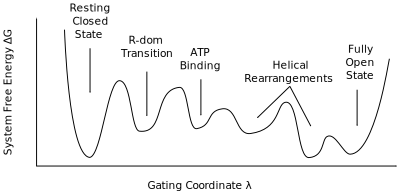
\includegraphics[width=\textwidth]{figures/drug_landscape_1.pdf}\\
	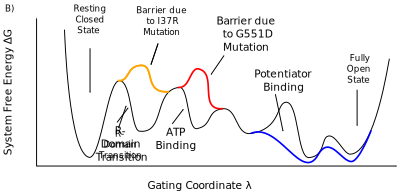
\includegraphics[width=\textwidth]{figures/drug_landscape_3.pdf}\\
	\end{center}
	\captionsetup{singlelinecheck = false, justification=raggedright}
	\caption[A physics motivated conceptual framework for how to think about the treatment of rare mutations by CFTR modulators ]{\textbf{physics motivated conceptual framework for how to think about the treatment of rare mutations by CFTR modulators}{This model was produced to explain the apparent ability of CFTR modulators to treat rare mutations with a diverse set of phenotypes. }}

\end{figure}

The ongoing discovery of rare mutations highlights the importance of this personalised approach to the treatment of CF. The process for developing potentiator class drugs was by studying the G551D mutation. Drugs that were found to restore function for this rare mutation are now widely used by sufferers of cystic fibrosis \cite{}. The study of rare mutations N1303K which currently do not respond to drugs may lead to the discovery of more effective compounds to treat cystic fibrosis such as. Thus, the approach to the treatment of Cystic Fibrosis is intersectional, as more rare mutations are discovered and treated the better the outcomes for all patients with Cystic Fibrosis will be. Each rare mutation sheds light on the function of CFTR and lets us understand and treat the root cause of the disease better.


This model makes clear what the pressing questions are in molecular cystic fibrosis research. These are three, primarily. Firstly and fundamentally, there is the task of finding the molecular details of the functional landscape in figure \ref{drug_action_figure}. Secondly, there is the elucidation of molecular misfunction of mutations. We must find \textit {where} in the functional landscape these mutations are causing issues, which will also tell us how. This will allow us to meaningfully group mutations into molecular theratypes. This leads us to the final task: Finding drugs to treat each of these theratypes. My personal opinion for the direction of each of these tasks is layed out in the subsequent sections.

Should the above model prove successful, such an approach approach to personalised medicine could  be considered when studying other monogenic diseases such as Muscular  Dystrophy, Sickle Cell Anemia and Huntington's disease \cite{}. Once single genes are understood the understanding could be built outward to encompass more complex diseases which involve the interactions between many genes such as diabetes and cancer. The future of personalised medicine is bright and it is possible that much of its breakthroughs will come from the molecular level.

\section{Outstanding fundamental questions about CFTR Function}
Firstly, there are controversies surrounding the structure of this protein. Primarily determining resolving the physiologically relevant conformations of TM8 and the conduction pathway of ions through CFTR.

Secondly, there are questions about how tightly the coupling of hydrolysis of ATP in the NBDs is to the conduction of ions.

\section{Grouping of Theratypes}
\begin{figure}
	\begin{center}
	%\includegraphics[angle=90,origin=c,width=0.5\textwidth]{figures/classes_mutations.pdf}\\
	\includegraphics[width=\textwidth]{figures/classes_mutations.pdf}\\
	\end{center}
	\captionsetup{singlelinecheck = false, justification=raggedright}
	\caption[Granular grouping of CF pathogenesis]{\textbf{Granular Grouping of Cystic Fibrosis Causing Mutations}{ Conventionally, CF genotypes are grouped into 7 classes of phenotype. These 7 classes, while useful are broad when one notes that the molecular details of misfunction can in fact be due to an array of factors. By realising that classification into a given class can be due to different factors we can gain a more complete  picture of the molecular cause of CF by delineating the molecular fingerprint of each mutation.}}

\end{figure}

As outlined in figure \ref{mutation_classes_figure} earlier, the molecular fingerprint of a mutation can be quite complex and ongoing work is needed to meaningfully group these mutations into more clinically meaningful categories. My prediction is that the conventional 6 classes will be more and more finely defined in order to choose CFTR modulators which are more specific to a patient's genotype and epithelial phenotype. 

\section{Resolving Drug Action}
Closely related to the above two categories is the mechanism of action for existing drugs and the development of new drugs. The reason we were able to discover potentiator class drugs is through the study of a rare mutation. High throughput screening of small molecules in restoring the gating class mutation G551D led to the discovery of gating class drugs. In this way we can see how the study of rare CF can lead to better outcomes for all sufferers of the disease. This is especially pertinent as more rare genotypes are discovered in non-Caucasian populations such as in Asia and the Middle East. 

Additionally, it should be obvious from this work that the action of these drugs is are highly dependent on the molecular function of CFTR. These small molecule drugs \textit{select} for a physiologically present conformation, so we would wish to design molecules which select for conformations which deliver the most clinic benefit. This is non-trivial and I believe  combination of careful molecular experiments, such as those of from the laboratories of Tzyh-Chang Hwang,  Christine E. Bear, L\'aszl\'o Csan\'ady and Paul Linsdell \cite{linsdell2018, csanady2019, zhang2017b}, and molecular simulations such as those found in this thesis and studies from the labs of John Paul Monron and Isabelle Callebaut \cite{Hoffmann2018}.

\chapter{Afterword}
\label{chap:Afterword}
\chapquote {}{}

 Thanks for coming along. I hope that towel came in handy \cite{adamd1979}. If you've made it this far I probably have you as a captive audience so I'm going to keep you just a bit longer. There are some things I'm going to tell you which are at the same time political, moral, practical and philosophical. The most important thing I will stress is the collaborative nature of science.

Just look at the reference list that follows, there are hundreds of publications listing thousands of authors. This likely millions, perhaps even billions of dollars of investment over the course of more than 100 years. However meager, my contributions to the study of CF and biophysics were only possible because of the patient and careful work of these people, from mathematicians to epidemiologists. Even the breakthroughs of the mythical lone genus aren't useful to anybody until implemented into a technology by thousands of workers. 

Throughout my studies I've needed to consult experts from all over science, who's brains have also been shaped by their own community of thousands. Every time I spoke with a friend in computer science I'd come away with a new trick to churn out simulations faster, every time I spoke to an astrophysicist I'd begin thinking in abstract hyperspaces which inspired me to push CFTR in a new direction (literally), when I spoke to cell biologists I'd come away motivated by the crazy things I hope to one day do help do to cells and every time I spoke to a biochemist I would something about proteins or CFTR which I could use for my simulations. I hope at the same time that some of my colleagues have also taken some inspiration from an increasingly unhinged physicist with a handful of GPUs. 

In these ways it has been invaluable to me to be able to stroll down the strangely long hallway of the school of physics to ask Zachary Picker for help with quantum mechanics or send an email across the world to ask Isabelle Callebaut what she thought about my dilated CFTR structure. Without such a diverse set of people I doubt I would have produced what I think is probably one of the few PhD dissertations which makes mention of both Schrodinger's wave equation and rectal biopsies. 

I want to make a quick note on the use of computers. I think, like pen and paper for the traditional mathematician, computers should be used as tools to think for the biologist. We have excellent theoretical models in biology but they are too complicated for the human brain to crank the handle on. I have found that automating parts of a workflow and cultivating a maintain library is like maintaining a tool belt. It makes you more useful. Plug into the matrix. It's fun.

They might have taken a long time but I hope I have shown you just how useful this kind of basic science can be . We're an adaptable species but we don't yet have any method of solving technical problems except this kind of patient investment

If my visa isn't denied I'm really looking forward to doing more of this stuff on TRP channels, maybe I'll make super chillies or something. .

In any case, thanks for sticking through X thousand words. I hope you learned a thing or two. .

Best, Miro

\include{./17-Appendix}

%%%%%%%%%%%%%%%%%%%%%%%
%% Bibliography      %%
%%%%%%%%%%%%%%%%%%%%%%%
\medskip
%\bibliographystyle{IEEEtran}
\printbibliography[heading=bibintoc]

%%%%%%%%%%%%%%%%%%%%%%%
%% Last Quote        %%
%%%%%%%%%%%%%%%%%%%%%%%



\end{document}
